% Template Laporan Skripsi/Thesis 
%
% @author  Andreas Febrian, Lia Sadita 
% @version 1.03
%
% Dokumen ini dibuat berdasarkan standar IEEE dalam membuat class untuk 
% LaTeX dan konfigurasi LaTeX yang digunakan Fahrurrozi Rahman ketika 
% membuat laporan skripsi. Konfigurasi yang lama telah disesuaikan dengan 
% aturan penulisan thesis yang dikeluarkan UI pada tahun 2008.
%

%
% Tipe dokumen adalah report dengan satu kolom. 
%
\documentclass[12pt, a4paper, onecolumn, oneside, final]{report}

\usepackage{amsthm,amsmath,amssymb}
\usepackage{lineno}
\usepackage{multirow}

\usepackage{caption}
\usepackage{booktabs}
\usepackage{graphicx}
\usepackage{float} 
\usepackage{adjustbox} 
\usepackage{hyperref}
\usepackage{indentfirst}
%\usepackage[authoryear]{natbib}

% \usepackage{subcaption}
% \usepackage{multirow}
% \usepackage{booktabs}
% \usepackage{colortbl}
\usepackage{array}
\usepackage{makecell}
\usepackage[table]{xcolor}  % biasanya sudah ada
\newcolumntype{L}[1]{>{\raggedright\arraybackslash}p{#1}}
\newcolumntype{C}[1]{>{\centering\arraybackslash}p{#1}}
\DeclareMathOperator*{\argmin}{arg\,min}
\DeclareMathOperator*{\argmax}{arg\,max}
\setlength{\headheight}{14.5pt}

% \usepackage{booktabs}
% \usepackage{multirow}
\usepackage{xcolor}
\usepackage{colortbl}
\usepackage{siunitx}

% Definisikan warna header tabel di preamble:
\definecolor{tableheader}{RGB}{220,230,242}
\definecolor{rowgray}{RGB}{245,245,245}

\usepackage{subcaption}
\usepackage{booktabs}
\usepackage{algorithm}
\usepackage{algpseudocode}
\usepackage{pgfplots}
\pgfplotsset{compat=1.18}
\usepackage{tikz}
\usetikzlibrary{arrows.meta, positioning, shapes.geometric}

\setlength{\abovedisplayskip}{0pt}
\setlength{\belowdisplayskip}{3pt}
\setlength{\abovedisplayshortskip}{0pt}
\setlength{\belowdisplayshortskip}{3pt}

\newcommand{\actplot}[4]{%
  \begin{tikzpicture}
    \begin{axis}[
      width=6.5cm, height=5cm,
      axis lines=center,
      xlabel={$v$}, ylabel={$\phi(v)$},
      tick label style={font=\footnotesize},
      domain=-4:4, samples=300,
      grid=major, grid style={dotted, gray!40},
      xmin=-4.2, xmax=4.2,
      ymin=#3, ymax=#4,
      title={\textbf{#1}}
    ]
    #2
    \end{axis}
  \end{tikzpicture}%
}
\usepackage[backend=biber, style=numeric, citestyle=authoryear]{biblatex}
\renewcommand{\nameyeardelim}{\addcomma\space}
\addbibresource{pustaka.bib}

\DefineBibliographyStrings{english}{
  and       = {dan},
  % andothers = {dkk\adddot},
}

% Buat "et al." jadi italic
\renewbibmacro*{name:andothers}{%
  \ifboolexpr{
    test {\ifnumequal{\value{listcount}}{\value{liststop}}}
    and
    test \ifmorenames
  }
    {\andothersdelim\bibstring[\mkbibitalic]{andothers}}
    {}}

% Load konfigurasi LaTeX untuk tipe laporan thesis
\usepackage{_internals/uithesis}

% Daftar pemenggalan suku kata dan istilah dalam LaTeX
\input{_internals/hype.indonesia}

% Load konfigurasi khusus untuk laporan yang sedang dibuat
%-----------------------------------------------------------------------------%
% Informasi Mengenai Dokumen
%-----------------------------------------------------------------------------%
% 
% Judul laporan. 
\var{\judul}{Judul Skripsi/Thesis/Disertasi}
% 
% Tulis kembali judul laporan, kali ini akan diubah menjadi huruf kapital
\Var{\Judul}{Judul Skripsi/Thesis/Disertasi}
% 
% Tulis kembali judul laporan namun dengan bahasa Ingris
\var{\judulInggris}{Unknown Title for Final Report/Thesis/Disertation}

% 
% Tipe laporan, dapat berisi Skripsi, Tugas Akhir, Thesis, atau Disertasi
\var{\type}{Skripsi}
% 
% Tulis kembali tipe laporan, kali ini akan diubah menjadi huruf kapital
\Var{\Type}{Skripsi}
% 
% Tulis nama penulis 
\var{\penulis}{Mohammad Raffy Zeidan}
% 
% Tulis kembali nama penulis, kali ini akan diubah menjadi huruf kapital
\Var{\Penulis}{Mohammad Raffy Zeidan}
% 
% Tulis NPM penulis
\var{\npm}{2206051462}
% 
% Tuliskan Fakultas dimana penulis berada
\Var{\Fakultas}{Matematika dan Ilmu Pengetahuan Alam}
\var{\fakultas}{Matematika dan Ilmu Pengetahuan Alam}
% 
% Tuliskan Program Studi yang diambil penulis
\Var{\Program}{STATISTIKA}
\var{\program}{Statistika}
% 
% Tuliskan tahun publikasi laporan
\Var{\bulan}{Mei}
\Var{\tahun}{2026}
% 
% Tuliskan gelar yang akan diperoleh dengan menyerahkan laporan ini
\var{\gelar}{Sarjana Statistika}
% 
% Tuliskan tanggal pengesahan laporan, waktu dimana laporan diserahkan ke 
% penguji/sekretariat
\var{\tanggalPengesahan}{XX Juli 2019} 
% 
% Tuliskan tanggal keputusan sidang dikeluarkan dan penulis dinyatakan 
% lulus/tidak lulus
\var{\tanggalLulus}{XX Juli 2019}
% 
% Tuliskan pembimbing 
\var{\pembimbing}{Prof. ???}
% 
% Alias untuk memudahkan alur penulisan paa saat menulis laporan
\var{\saya}{Penulis}

%-----------------------------------------------------------------------------%
% Judul Setiap Bab
%-----------------------------------------------------------------------------%
% 
% Berikut ada judul-judul setiap bab. 
% Silahkan diubah sesuai dengan kebutuhan. 
% 
\Var{\kataPengantar}{Kata Pengantar}
\Var{\babSatu}{Pendahuluan}
\Var{\babDua}{Landasan Teori}
\Var{\babTiga}{METODE MODEL JOINT SENTIMENT-TOPIC BERBASIS MULTITASK
LEARNING}
\Var{\babEmpat}{HASIL DAN SIMULASI DAN PEMBAHASAN}
\Var{\kesimpulan}{Kesimpulan}

% Daftar istilah yang mungkin perlu ditandai 
\input{istilah}

% Awal bagian penulisan laporan
\begin{document}
%
% Sampul Laporan
\input{_internals/sampul}

%
% Gunakan penomeran romawi
\pagenumbering{roman}

%
% load halaman judul dalam
\addChapter{HALAMAN JUDUL}
\input{_internals/judul_dalam}

%
% setelah bagian ini, halaman dihitung sebagai halaman ke 2
\setcounter{page}{2}

%
% load halaman pengesahan
\addChapter{LEMBAR PERSETUJUAN}
\input{src/00-front_matter/01-persetujuan}
%
% load halaman orisinalitas 
\addChapter{LEMBAR PERNYATAAN ORISINALITAS}
\input{src/00-front_matter/02-orisinalitas}
%
%
\addChapter{LEMBAR PENGESAHAN}
%
% Halaman Pengesahan Sidang
%
% @author  Andreas Febrian, Andre Tampubolon 
% @version 1.02
%

\chapter*{HALAMAN PENGESAHAN}

\vspace*{0.4cm}
\noindent 

\noindent
\begin{tabular}{ll p{9cm}}
	\type~ini diajukan oleh&: & \\
	Nama&: & \penulis \\
	NPM&: & \npm \\
	Program Studi&: & \program \\
	Judul \type&: & \judul \\
\end{tabular} \\

\vspace*{1.0cm}

\noindent \bo{Telah berhasil dipertahankan di hadapan Dewan Penguji 
dan diterima sebagai bagian persyaratan yang diperlukan untuk 
memperoleh gelar \gelar~pada Program Studi \program, Fakultas 
\fakultas, Universitas Indonesia.}\\[0.2cm]

\begin{center}
	\bo{DEWAN PENGUJI}
\end{center}

\vspace*{0.3cm}

\begin{tabular}{l l l l}
	& & & \\
	Pembimbing I & : & Prof. Dr.rer.nat. Hendri Murfi, S.Si., M.Kom. & (\hspace*{3.0cm}) \\
	& & & \\
	Pembimbing II & : & Dra. Nora Hariadi, M.Si. & (\hspace*{3.0cm}) \\
	& & & \\
	Penguji I & : & Prof. Alhadi Bustamam, S.Si., M.Kom., Ph.D. & (\hspace*{3.0cm}) \\
	& & & \\
	Penguji II & : & Kurnia Susvitasari, S.Si., M.Sc., Ph.D. & (\hspace*{3.0cm}) \\
\end{tabular}\\


\vspace*{2.0cm}

\begin{tabular}{ll l}
	Ditetapkan di&: & Depok\\
	Tanggal&: & \tanggalLulus \\
\end{tabular}


\newpage

%
%
\addChapter{\kataPengantar}
%-----------------------------------------------------------------------------%
\chapter*{Kata Pengantar}
%-----------------------------------------------------------------------------%
Puji syukur penulis panjatkan kepada Tuhan Yang Maha Esa atas segala berkat 
dan rahmat-Nya sehingga penulis dapat menyelesaikan skripsi ini dengan 
sebaik-baiknya. 
Selama masa penulisan skripsi ini, penulis telah mendapat banyak dukungan, 
doa, bantuan, inspirasi, dan motivasi dari berbagai pihak. 
Untuk itu, penulis ingin mengucapkan terima kasih kepada:
\begin{enumerate}
    \item Bapak Prof.\ Dr.\ rer.\ nat.\ Hendri Murfi, S.Si., M.Kom.\ selaku 
        Dosen Pembimbing I yang telah membimbing penulis dengan penuh 
        kesabaran dan ketulusan. Arahan dan ilmu yang beliau berikan tidak 
        hanya membantu penulis menyelesaikan penelitian ini, tetapi juga 
        membentuk cara penulis berpikir dalam menghadapi permasalahan 
        secara lebih mendalam.
    \item Ibu Dra.\ Nora Hariadi, M.Si.\ selaku Dosen Pembimbing II yang 
        dengan teliti telah memberikan arahan terkait tata cara penulisan 
        skripsi. Perhatian beliau terhadap setiap detail penulisan sangat 
        membantu penulis dalam menyusun karya ilmiah yang sistematis dan 
        sesuai kaidah akademik.
    \item Bapak Prof.\ Alhadi B., S.Si., M.Kom., Ph.D.\ selaku Dosen Penguji 
        I yang telah memberikan kritik dan saran yang tajam dan membangun, 
        sehingga mendorong penulis untuk berpikir lebih kritis dalam 
        menyempurnakan skripsi ini.
    \item Ibu Dr.\ Nahlia Rakhmawati, M.Si.\ selaku Dosen Penguji II 
        yang telah memberikan masukan dan perspektif yang memperkaya 
        pembahasan dalam skripsi ini.
    \item Ibu Prof.\ Dr.\ Titin Siswantining, D.E.A.\ selaku Dosen 
        Pembimbing Akademis yang senantiasa memberikan arahan, nasihat, 
        dan dukungan selama penulis menjalani masa perkuliahan.
    \item Orang tua penulis, Bapak Timu dan Ibu Yuyun Dharmayanti, yang 
        telah memberikan segalanya. Doa, dukungan, dan kesediaan untuk 
        selalu ada baik di saat semangat maupun di saat lelah menjadi 
        kekuatan terbesar yang menopang penulis hingga sampai di titik ini.
    \item Teman-teman Group DKM (Bagja College) yang telah menjadi bagian 
        dari perjalanan penulis sejak masa SMA dan kebersamaannya terus 
        berlanjut hingga saat ini.
    \item Farhan, Dafa, Nicholas, dan Aditya, teman sepersemesteran yang 
        hadir dari hari-hari pertama kuliah hingga akhir. Kehadiran mereka 
        membuat perjalanan yang panjang ini terasa lebih ringan.
    \item RISTEK Fasilkom UI yang melalui kompetisi \textit{data science}-nya 
        telah membuka jalan bagi penulis menuju dunia yang kini menjadi 
        bagian besar dari kehidupan akademik dan karier penulis.
    \item PT Profina Edvisor yang telah memberikan kepercayaan dan ruang 
        bagi penulis untuk tumbuh sebagai seorang \textit{data scientist}, 
        serta dukungan yang tidak pernah surut selama proses penyelesaian 
        skripsi ini.
    \item Seluruh pihak yang tidak dapat disebutkan satu per satu, yang 
        dengan caranya masing-masing telah turut mengambil peran dalam 
        perjalanan panjang ini.
\end{enumerate}

Penulis menyadari bahwa skripsi ini masih memiliki keterbatasan dan 
kekurangan, baik dari segi penulisan maupun substansi keilmuan. 
Oleh karena itu, kritik dan saran yang membangun sangat penulis harapkan 
sebagai bahan perbaikan ke depan. 
Penulis berharap skripsi ini dapat bermanfaat bagi pembaca dan menjadi 
bagian dari kontribusi nyata dalam pengembangan ilmu pengetahuan, 
khususnya di bidang yang dikaji dalam penelitian ini.

\vspace*{0.5cm}
\noindent Depok, 30 Juni 2026\\[0.1cm]
\penulis
%
%
\addChapter{LEMBAR PERSETUJUAN PUBLIKASI ILMIAH}
\chapter*{Halaman Pernyataan Persetujuan Publikasi Tugas Akhir untuk Kepentingan Akademis}

\vspace*{-1.2cm} % atur sesuai kebutuhan
\noindent\rule{\textwidth}{2pt} % garis horizontal

\vspace*{0.3cm}

\noindent
Sebagai sivitas akademik Universitas Indonesia, saya yang bertanda tangan di bawah ini:

\vspace*{0.3cm}
\begin{tabular}{p{3.2cm} l p{8cm}}
    Nama          & : & \penulis \\
    NPM           & : & \npm \\
    Program Studi & : & \program \\
    Departemen    & : & \departemen \\
    Fakultas      & : & \fakultas \\
    Jenis Karya   & : & \type \\
\end{tabular}
\vspace*{0.3cm}

\noindent demi pengembangan ilmu pengetahuan, menyetujui untuk memberikan kepada Universitas Indonesia \textbf{Hak Bebas Royalti Noneksklusif (\textit{Non-exclusive Royalty Free Right})} atas karya ilmiah saya yang berjudul:

\vspace*{0.3cm}
\begin{center}
    \judul
\end{center}
\vspace*{0.3cm}

\noindent beserta perangkat yang ada (jika diperlukan). Dengan Hak Bebas Royalti Noneksklusif ini, Universitas Indonesia berhak menyimpan, mengalihmedia/formatkan, mengelola dalam bentuk pangkalan data (\textit{data base}), merawat, dan memublikasikan tugas akhir saya selama tetap mencantumkan nama saya sebagai penulis/pencipta dan sebagai pemilik Hak Cipta.

\vspace*{0.4cm}
\noindent Demikian pernyataan ini saya buat dengan sebenarnya.

\vspace*{0.8cm}
\begin{center}
    \begin{tabular}{l c l}
        Dibuat di    & : & Depok \\
        Pada tanggal & : & \tanggalPengesahan \\
    \end{tabular}

    \vspace*{0.3cm}
    Yang menyatakan

    \vspace*{1.5cm}
    (\penulis)
\end{center}
\newpage
%
% 
\addChapter{ABSTRAK}
\chapter*{Abstrak}
\vspace*{0.2cm}

{
\setlength{\parindent}{0pt}
\noindent
Nama: \penulis\par
Program Studi: \program\par
Judul: \judul\par
\medskip

\noindent
Pertumbuhan data teks dari platform digital, seperti ulasan produk dan media
sosial, mendorong kebutuhan akan metode otomatis yang mampu menganalisis
sentimen dan mengidentifikasi topik secara bersamaan. Pendekatan analisis
sentimen konvensional umumnya mengasumsikan satu sentimen untuk setiap
dokumen sehingga belum mampu merepresentasikan ulasan yang membahas lebih
dari satu topik. Penelitian ini mengembangkan model \textit{Joint
Document-Level Sentiment--Topic} berbasis \textit{Deep Embedded Clustering}
(JDST-DEC) yang mengintegrasikan analisis sentimen dan pemodelan topik
secara \textit{end-to-end} dalam kerangka \textit{Multi-Task Learning}
(MTL), menggunakan satu \textit{shared encoder} berbasis BERT dan DEC
sebagai \textit{topic head} untuk membentuk representasi topik dari
representasi laten yang dihasilkan encoder. Pelatihan dilakukan dalam dua
tahap, yaitu pra-pelatihan \textit{autoencoder} untuk membentuk representasi
laten, kemudian optimisasi gabungan menggunakan \textit{sentiment loss}
berbasis \textit{cross-entropy} dan \textit{clustering loss} berbasis KL
\textit{divergence}. Evaluasi dilakukan pada dataset IMDB dan Yelp dengan
variasi jumlah topik $K=30$, $50$, dan $80$. Pada tugas klasifikasi
sentimen, JDST-DEC memperoleh F1-\textit{score} terbaik sebesar 0{,}8986
pada IMDB dan 0{,}9020 pada Yelp ($K=50$), lebih tinggi dibandingkan
NN-BERT (0{,}8612 dan 0{,}8715). Pada tugas pemodelan topik, JDST-DEC
menghasilkan kualitas topik yang lebih baik dibandingkan MTL-GUI pada
beberapa konfigurasi, namun masih berada di bawah BERTopic-KMeans
berdasarkan metrik \textit{Topic Coherence} (TC-NPMI) dan \textit{Topic
Diversity}. Hasil ini menunjukkan bahwa \textit{Deep Embedded Clustering}
berhasil diintegrasikan ke dalam kerangka JDST dan mampu meningkatkan
performa klasifikasi sentimen dibandingkan model \textit{single-task},
meskipun kualitas representasi topik masih berada di bawah metode
pemodelan topik khusus.
\medskip

\noindent
\textbf{Kata kunci}: \textit{Deep Embedded Clustering},
\textit{Joint Document-Level Sentiment--Topic Modeling},
\textit{Multi-Task Learning}, \textit{BERT}.
}

\newpage

%
%
%-----------------------------------------------------------------------------%
\chapter*{Extended Abstract}
\addcontentsline{toc}{chapter}{Extended Abstract}
%-----------------------------------------------------------------------------%

\renewcommand{\thetable}{\arabic{table}}
\renewcommand{\thefigure}{\arabic{figure}}
\setcounter{figure}{0}
\setcounter{table}{0}

\vspace*{0.2cm}
{
\setlength{\parindent}{0pt}

\begin{center}
{\large\textbf{EXTENDED ABSTRACT}}

\medskip
{\normalsize\textbf{Undergraduate Thesis}}

\medskip
{\normalsize\textbf{\textit{\judulInggris}}}

\medskip
\textbf{Student Name} : \penulis \\
\textbf{Student ID Number (NPM)} : 2206051462 \\
\textbf{Study Program} : \program
\end{center}

\bigskip

% #20 opening gap sentence added
Every day, review platforms and social media generate enormous volumes of
user-generated text. Automatically extracting sentiment and thematic content
from this data has become a central challenge in Natural Language Processing
(NLP). Conventional document-level sentiment analysis reduces each document
to a single polarity label, which overlooks the fact that a review often
discusses multiple aspects with differing opinions. Yet existing joint
sentiment-topic approaches either require aspect-level supervision or rely
on pipeline architectures that do not allow the two objectives to reinforce
each other during training. This limitation motivates end-to-end joint
approaches that simultaneously model sentiment and topics, offering richer
output without requiring aspect-level annotations.

% #17 JDST-DEC name bolded on first mention; #3 "summarised"; #4 loss weight extended; #5 K notation
To address this, the present study proposes a \textit{Joint Document-Level
Sentiment-Topic} model based on \textit{Deep Embedded Clustering}
(\textbf{JDST-DEC}) within a \textit{Multi-Task Learning} (MTL) framework.
The model operates in two stages. In the first stage, the 768-dimensional
\texttt{[CLS]} representation extracted by a frozen BERT encoder, which
reduces computational cost and preserves stable pre-trained
representations, is fed into a symmetric fully connected autoencoder
with architecture $768 \to 2022 \to 2022 \to 256$, trained using mean
squared error (MSE) to learn a compact 256-dimensional latent
representation. In the second stage, this latent space is jointly optimised
for sentiment classification via cross-entropy loss
($\mathcal{L}_{\text{sent}}$) and topic clustering via DEC with KL
divergence loss ($\mathcal{L}_{\text{clust}}$), under the joint objective:
\[
    \mathcal{L} = \eta\,\mathcal{L}_{\text{sent}} +
    \gamma\,\mathcal{L}_{\text{clust}}, \qquad \eta = \gamma = 0{.}5,
\]
where equal weighting balances the sentiment classification and clustering
objectives without favouring either. Cluster centroids are initialised
using \textit{k}-means on the pre-trained latent space. The overall
research workflow is summarised in Figure~1.

% #2 caption no longer has "Figure 1." prefix
\begin{figure}[H]
    \centering
    
\includegraphics[width=0.82\textwidth]{assets/pics/other/Flowchart.png}
    \caption{Schematic diagram of the research framework.}
    \label{fig:ea_workflow}
\end{figure}

% #1 fairness statement; #5 K notation; #18 MTL-GUI consistent
Experiments were conducted on two benchmark datasets: IMDB Movie Reviews
\parencite{maas2011} (50{,}000 reviews) and the Yelp Review Dataset
\parencite{zhang2015} (30{,}000 reviews), both with binary sentiment labels.
Three topic cardinalities $K\in\{30,50,80\}$ were evaluated.
\textbf{JDST-DEC} was compared against NN-BERT as a single-task sentiment
baseline, MTL-GUI \parencite{gui2022mtml}, BERTopic-HDBSCAN, and
BERTopic-KMeans. All baselines were re-evaluated under identical dataset
splits and evaluation protocols to ensure a fair comparison. Sentiment
performance was measured using accuracy and F1-score; topic quality was
assessed using \textit{Topic Coherence} based on NPMI (TC-NPMI) and
\textit{Topic Diversity} (TD).

Pre-training results show that reconstruction loss drops sharply in the
early epochs and stabilises after epoch~20, reaching final training losses
of approximately $1{.}41 \times 10^{-4}$ on IMDB and $1{.}55 \times 10^{-4}$
on Yelp. Validation loss remains close to training loss throughout, indicating
no overfitting. Selected pre-training loss values are shown in Table~1.

\begin{table}[H]
    \centering
    \caption{Selected pre-training \textit{loss} values on the IMDB and
    Yelp datasets.}
    \label{tab:ea_pretrain}
    \renewcommand{\arraystretch}{1.15}
    \begin{tabular}{ccccc}
        \toprule
        \multirow{2}{*}{\textbf{Epoch}}
          & \multicolumn{2}{c}{\textbf{IMDB}}
          & \multicolumn{2}{c}{\textbf{Yelp}} \\
        \cmidrule(lr){2-3}\cmidrule(lr){4-5}
          & \textit{Train} & \textit{Val.}
          & \textit{Train} & \textit{Val.} \\
        \midrule
         1  & $2{.}370 \times 10^{-3}$ & $2{.}544 \times 10^{-3}$
            & $3{.}790 \times 10^{-3}$ & $4{.}062 \times 10^{-3}$ \\
        10  & $3{.}780 \times 10^{-4}$ & $4{.}120 \times 10^{-4}$
            & $2{.}780 \times 10^{-4}$ & $3{.}040 \times 10^{-4}$ \\
        20  & $1{.}370 \times 10^{-4}$ & $1{.}550 \times 10^{-4}$
            & $1{.}670 \times 10^{-4}$ & $1{.}860 \times 10^{-4}$ \\
        30  & $1{.}410 \times 10^{-4}$ & $1{.}590 \times 10^{-4}$
            & $1{.}550 \times 10^{-4}$ & $1{.}730 \times 10^{-4}$ \\
        \bottomrule
    \end{tabular}
\end{table}

% #6 "percentage points"; #19 consistent number format
For sentiment classification, \textbf{JDST-DEC} consistently outperforms
NN-BERT and MTL-GUI across all values of $K$ on both datasets (Table~2).
On IMDB, \textbf{JDST-DEC} achieves its best F1-score of 0.8986 at $K = 50$,
compared with 0.8612 for NN-BERT and 0.8317 for MTL-GUI, corresponding to
improvements of approximately 3.7 and 6.7 percentage points respectively.
On Yelp, \textbf{JDST-DEC} reaches an F1-score of 0.9020 at $K = 50$,
compared with 0.8715 and 0.8401, representing gains of approximately 3.1 and
6.2 percentage points. Performance remains stable across all values of $K$,
indicating that sentiment classification quality is relatively insensitive
to topic cardinality. Among the compared methods,
\textbf{JDST-DEC} achieves the highest sentiment scores on Yelp and
competitive results on IMDB.

% #16 dagger notation added to method name; #15 identical evaluation settings in footnote
% #16 dagger notation added to method name; #15 identical evaluation settings in footnote
\begin{table}[H]
\centering
\caption{Comparison of sentiment classification results on IMDB and Yelp.}
\label{tab:ea_sentiment}
\small
\renewcommand{\arraystretch}{1.55}
\setlength{\tabcolsep}{6pt}
\begin{adjustbox}{width=\textwidth}
\begin{tabular}{|l|cc|cc|cc|cc|cc|cc|}
\hline
\multirow{2}{*}{Method}
  & \multicolumn{6}{c|}{IMDB}
  & \multicolumn{6}{c|}{Yelp} \\
\cline{2-13}
  & \multicolumn{2}{c|}{}
  & \multicolumn{2}{c|}{Acc \qquad F1}
  & \multicolumn{2}{c|}{}
  & \multicolumn{2}{c|}{}
  & \multicolumn{2}{c|}{Acc \qquad F1}
  & \multicolumn{2}{c|}{} \\
\hline
NN-BERT
  & \multicolumn{6}{c|}{0.8581 \qquad 0.8612}
  & \multicolumn{6}{c|}{0.8664 \qquad 0.8715} \\
\hline
  & \multicolumn{2}{c|}{$K=30$}
  & \multicolumn{2}{c|}{$K=50$}
  & \multicolumn{2}{c|}{$K=80$}
  & \multicolumn{2}{c|}{$K=30$}
  & \multicolumn{2}{c|}{$K=50$}
  & \multicolumn{2}{c|}{$K=80$} \\
\cline{2-13}
  & Acc & F1
  & Acc & F1
  & Acc & F1
  & Acc & F1
  & Acc & F1
  & Acc & F1 \\
\hline
MTL-GUI
  & 0.8327 & 0.8326
  & 0.8317 & 0.8317
  & 0.8334 & 0.8334
  & 0.8385 & 0.8385
  & 0.8380 & 0.8380
  & 0.8402 & 0.8401 \\
\hline
\textbf{JDST-DEC}
  & \cellcolor{green!25}\textbf{0.8957} & \cellcolor{green!25}\textbf{0.8963}
  & \cellcolor{green!25}\textbf{0.8967} & \cellcolor{green!25}\textbf{0.8986}
  & \cellcolor{green!25}\textbf{0.8941} & \cellcolor{green!25}\textbf{0.8930}
  & \cellcolor{green!25}\textbf{0.8965} & \cellcolor{green!25}\textbf{0.8944}
  & \cellcolor{green!25}\textbf{0.8983} & \cellcolor{green!25}\textbf{0.9020}
  & \cellcolor{green!25}\textbf{0.8935} & \cellcolor{green!25}\textbf{0.8953} \\
\hline
\end{tabular}
\end{adjustbox}
\vspace{0.3em}
\noindent{\footnotesize
  \colorbox{green!25}{\,\,} highest value in column;
  
  All baselines evaluated under identical dataset splits and protocols.}
\end{table}

% #7 "which is expected" removed
For topic modelling, BERTopic achieves the highest TD values across most
configurations (Table~3), with BERTopic-KMeans reaching 0.9567 on IMDB
at $K = 30$. For TC-NPMI, BERTopic-HDBSCAN leads at $K = 30$ and $K = 50$
on IMDB, while BERTopic-KMeans leads at $K = 80$. On Yelp, BERTopic
variants achieve the highest TC-NPMI values across all settings.
\textbf{JDST-DEC} produces lower TC-NPMI and TD values than BERTopic, as
joint optimisation prioritises sentiment-discriminative representations
over purely coherent topic structures. Among the joint models,
\textbf{JDST-DEC} consistently outperforms MTL-GUI on both metrics and
both datasets across every value of $K$.

% #16 dagger in topic table; #15 footnote; #17 JDST-DEC bolded
\begin{table}[H]
\centering
\caption{Comparison of topic modelling results on IMDB and Yelp.}
\label{tab:ea_topic}
\small
\renewcommand{\arraystretch}{1.55}
\setlength{\tabcolsep}{6pt}
\begin{adjustbox}{width=\textwidth}
\begin{tabular}{|l|cc|cc|cc|cc|cc|cc|}
\hline
\multirow{3}{*}{Method}
  & \multicolumn{6}{c|}{IMDB}
  & \multicolumn{6}{c|}{Yelp} \\
\cline{2-13}
  & \multicolumn{2}{c|}{$K=30$}
  & \multicolumn{2}{c|}{$K=50$}
  & \multicolumn{2}{c|}{$K=80$}
  & \multicolumn{2}{c|}{$K=30$}
  & \multicolumn{2}{c|}{$K=50$}
  & \multicolumn{2}{c|}{$K=80$} \\
\cline{2-13}
  & TC-NPMI & TD
  & TC-NPMI & TD
  & TC-NPMI & TD
  & TC-NPMI & TD
  & TC-NPMI & TD
  & TC-NPMI & TD \\
\hline
BERTopic-HDBSCAN
  & \cellcolor{green!25}\textbf{0.1714} & 0.7966
  & \cellcolor{green!25}\textbf{0.1823} & 0.7680
  & 0.1751 & 0.7625
  & 0.1092 & 0.7233
  & \cellcolor{green!25}\textbf{0.1666} & \cellcolor{green!25}\textbf{0.7041}
  & \cellcolor{green!25}\textbf{0.1646} & \cellcolor{green!25}\textbf{0.6671} \\
\hline
BERTopic-KMeans
  & 0.1566 & \cellcolor{green!25}\textbf{0.9567}
  & 0.1596 & \cellcolor{green!25}\textbf{0.9000}
  & \cellcolor{green!25}\textbf{0.1874} & \cellcolor{green!25}\textbf{0.8413}
  & 0.1077 & \cellcolor{green!25}\textbf{0.7800}
  & 0.1120 & 0.6740
  & 0.1465 & 0.6438 \\
\hline
MTL-GUI
  & 0.0200 & 0.5833
  & 0.0108 & 0.5800
  & 0.0060 & 0.4913
  & \cellcolor{green!25}\textbf{0.1578} & 0.6600
  & 0.1086 & 0.6720
  & 0.1123 & 0.5000 \\
\hline
\textbf{JDST-DEC}
  & 0.0803 & 0.2256
  & 0.0551 & 0.2100
  & 0.0675 & 0.2875
  & 0.0788 & 0.3267
  & 0.0369 & 0.2280
  & 0.0563 & 0.3150 \\
\hline
\end{tabular}
\end{adjustbox}
\vspace{0.3em}
\noindent{\footnotesize
  \colorbox{green!25}{\,\,} highest value in column;
  
  All baselines evaluated under identical dataset splits and protocols.}
\end{table}

% #8 training dynamics interpretation added
Analysis of the joint training dynamics shows that
$\mathcal{L}_{\text{sent}}$ decreases consistently from early iterations,
while $\mathcal{L}_{\text{clust}}$ tends to increase throughout training.
This reflects the DEC mechanism, in which the target distribution is
iteratively updated based on current cluster assignments, keeping the
KL divergence active and allowing the cluster structure to continue
evolving during joint optimisation. The opposing trends of the two losses
suggest that the model progressively trades raw reconstruction accuracy
for a latent geometry that is simultaneously sentiment-discriminative and
cluster-coherent.

% #9 fewer token examples; #10 "lexical polarity"
Interpretability analysis using occlusion-based token attribution on the
Yelp dataset ($K = 30$) shows that tokens such as \textit{``super''} and
\textit{``average''} carry attributions consistent with their expected
polarity, while certain tokens exhibit signs inconsistent with their
lexical polarity, indicating that the model captures context-sensitive
interactions rather than relying on surface-form cues alone.

% #11 frozen encoder limitation added
\paragraph{Limitations.}
The current study has several limitations. The experiments are limited to
binary sentiment classification on English-language datasets; performance
on multi-class or multilingual settings remains to be established. The
use of a frozen BERT encoder, while computationally efficient, may limit
the model's ability to adapt its representations to domain-specific
sentiment signals. The autoencoder architecture and DEC objective are
fixed throughout training, and it is unclear whether deeper or alternative
architectures would improve topic quality without sacrificing sentiment
accuracy. Finally, evaluation relies on automated topic metrics
(TC-NPMI, TD), which do not fully capture human judgements of topic
usefulness.

% #12 encoder fine-tuning added to future work
In future work, these limitations motivate exploring encoder fine-tuning
strategies that balance adaptation with stability, deeper autoencoder
architectures and alternative clustering objectives to improve topic
diversity, and extensions to multilingual and multi-class sentiment
settings. Incorporating aspect-level evaluation would further
characterise the granularity of the learned topic representations.

% #13 impact sentence added
In conclusion, \textbf{JDST-DEC} demonstrates an effective mechanism for
joint sentiment-topic learning: integrating DEC into an MTL framework
with a frozen BERT encoder improves sentiment classification over both
single-task and existing joint-model baselines, and produces interpretable
topic clusters, all without requiring aspect-level annotations. By showing
that a single latent space can serve both objectives simultaneously, this
work opens a practical path toward richer, annotation-efficient document
understanding in large-scale review and social-media settings.

\bigskip
% #14 Topic Modeling keyword added
\noindent\textbf{Keywords}: \textit{Deep Embedded Clustering},
\textit{Joint Document-Level Sentiment-Topic Modeling},
\textit{Multi-Task Learning}, \textit{Topic Modeling},
\textit{BERT}.

}

% Restore chapter-prefixed numbering after abstract
\renewcommand{\thetable}{\thechapter.\arabic{table}}
\renewcommand{\thefigure}{\thechapter.\arabic{figure}}

\newpage

%
% Daftar isi, gambar, dan tabel
%
\phantomsection
\tableofcontents
\clearpage
\phantomsection
\listoffigures
\clearpage
\phantomsection
\listoftables
\clearpage
\phantomsection
\listoflistings
\clearpage

%
% Gunakan penomeran Arab (1, 2, 3, ...) setelah bagian ini.
%
\pagenumbering{arabic}

%
%
%
%-----------------------------------------------------------------------------%
\chapter{\babSatu}
%-----------------------------------------------------------------------------%


%-----------------------------------------------------------------------------%
\section{Latar Belakang}
%-----------------------------------------------------------------------------%

Dunia kontemporer dibanjiri oleh arus deras informasi tekstual yang dihasilkan setiap saat, bersumber dari platform media sosial, ulasan daring, artikel berita, repositori ilmiah, dan banyak lagi. Kumpulan data tekstual masif ini, yang sebagian besar tidak terstruktur, mengandung potensi pengetahuan yang signifikan mengenai sentimen masyarakat, dinamika pasar, hingga tren diskursus publik. Akan tetapi, volume dan keragaman data tersebut menjadikan analisis manual suatu hal yang tidak praktis dan efisien. Menjawab tantangan ini, disiplin \textit{Natural Language Processing} (NLP), sebagai bagian dari kecerdasan artifisial yang menjembatani komunikasi antara mesin dan bahasa alami manusia, hadir menawarkan metodologi komputasional untuk mengolah dan memahami data linguistik dalam skala besar.

\bigskip

Dalam spektrum kapabilitas NLP, dua teknik yang memiliki relevansi tinggi untuk mengekstrak makna dari himpunan data tekstual adalah analisis sentimen (\textit{Sentiment Analysis}) dan pemodelan topik (\textit{Topic Modeling}) \parencite{blei2003latent}. Analisis sentimen secara khusus dirancang untuk menyelidiki dan menentukan muatan subjektif atau nada emosional yang terkandung dalam suatu teks, lalu menggolongkannya sebagai ekspresi positif, negatif, ataupun netral. Pengaplikasian teknik ini sangat berharga untuk melacak citra merek, menganalisis tanggapan konsumen, memetakan opini publik terkait isu tertentu, serta mengidentifikasi ujaran problematik. Kemampuan mengukur sentimen secara kolektif memberikan landasan bagi entitas bisnis maupun riset untuk memahami persepsi dan mengambil langkah strategis.

\bigskip

Di sisi lain, pemodelan topik menangani tugas komplementer, yakni mengungkap tema-tema atau pokok bahasan esensial yang tersembunyi (\textit{latent thematic structures}) di dalam koleksi dokumen berjumlah besar, atau sering disebut \textit{corpora} \parencite{blei2003latent}. Berbeda dengan fokus pada nuansa afektif per teks, tujuan utama pemodelan topik adalah menyajikan intisari tematik dari keseluruhan data. Kegunaannya terbentang luas, mulai dari fasilitasi eksplorasi dan pengorganisasian arsip digital, identifikasi pola baru dalam korpus literatur atau berita, hingga penyempurnaan sistem rekomendasi konten dan pemahaman struktur narasi dalam skala makro. Dengan mengabstraksikan topik-topik dominan, metode ini membantu mereduksi kompleksitas informasi dan menyajikan gambaran umum konten. Walaupun memiliki fokus yang berbeda, kedua pendekatan ini berpotensi menghasilkan pemahaman yang lebih komprehensif jika diintegrasikan, menyingkap \textit{apa} subjek pembicaraan sekaligus \textit{bagaimana} pandangan atau perasaan terhadap subjek tersebut.

\bigskip

Pendekatan tradisional dalam pemodelan topik, seperti \textit{Latent Dirichlet Allocation} (LDA), umumnya berbasis probabilistik dan mengandalkan metode faktorisasi matriks untuk mengidentifikasi distribusi kata dalam topik \parencite{blei2003latent, blei2012probabilistic}. Meskipun metode ini telah terbukti efektif dalam banyak kasus, keterbatasannya dalam menangkap hubungan semantik yang kompleks dalam teks membuatnya kurang optimal untuk tugas yang lebih kompleks, seperti klasifikasi sentimen yang dilakukan secara simultan dengan deteksi topik. Salah satu kelemahan utama pendekatan probabilistik seperti LDA adalah skalabilitasnya yang terbatas, terutama saat diaplikasikan pada \textit{dataset} berukuran besar dengan dimensi fitur tinggi \parencite{boydgraber2017synthetic}. Selain itu, model berbasis probabilistik sering kali memerlukan waktu komputasi yang signifikan dan sulit diadaptasi untuk menangani data teks modern yang bersifat dinamis dan tidak terstruktur \parencite{mcauliffe2008supervised}.

\bigskip

Dalam klasifikasi sentimen, pendekatan berbasis pembelajaran mendalam (\textit{deep learning}) telah menunjukkan keunggulan signifikan dibandingkan metode tradisional. Salah satu model yang paling efektif adalah \textit{Bidirectional Encoder Representations from Transformers} (BERT), yang mampu memahami konteks kata dalam teks dengan mempertimbangkan hubungan antar kata di kedua arah (\textit{bidirectional}) \parencite{devlin2018bert}. BERT telah banyak digunakan dalam tugas-tugas NLP dan terbukti unggul dalam klasifikasi sentimen, menghasilkan akurasi yang lebih tinggi dibandingkan pendekatan berbasis fitur atau metode statistik konvensional \parencite{sun2019fine}.

\bigskip

Seiring dengan berkembangnya model \textit{deep learning}, pendekatan berbasis jaringan saraf telah terbukti lebih unggul dalam menangani data teks yang tidak terstruktur dibandingkan metode berbasis probabilistik seperti LDA \parencite{mikolov2013efficient}. Model \textit{neural network} dapat mengekstrak representasi semantik yang lebih kaya dan menangkap hubungan kontekstual antar kata dalam teks dengan lebih baik \parencite{zhang2020neural}. Selain itu, pendekatan \textit{neural network} dapat mengatasi keterbatasan skalabilitas pada metode probabilistik karena dapat memanfaatkan arsitektur yang lebih efisien seperti \textit{transformers} dan teknik \textit{embedding} untuk mengurangi dimensi data \parencite{vaswani2017attention}.

\bigskip

Salah satu pendekatan berbasis \textit{neural network} yang semakin populer dalam pemodelan topik adalah \textit{BERTopic}. Berbeda dengan LDA yang hanya mengandalkan distribusi kata untuk menentukan topik, \textit{BERTopic} memanfaatkan representasi teks dari model \textit{transformer} seperti BERT untuk menangkap hubungan semantik yang lebih dalam antar kata \parencite{grootendorst2022bertopic}. Metode ini menggabungkan \textit{embedding} berbasis \textit{transformer} dengan teknik klasterisasi seperti \textit{UMAP} dan \textit{HDBSCAN} untuk mengidentifikasi topik secara lebih akurat dan stabil, bahkan dalam \textit{dataset} berukuran besar atau dengan struktur yang kompleks. Keunggulan utama \textit{BERTopic} dibandingkan LDA adalah kemampuannya dalam menangani variasi bahasa yang lebih luas, memahami sinonim dan kontekstualisasi kata, serta tidak bergantung pada asumsi distribusi kata seperti pada metode probabilistik \parencite{grootendorst2022bertopic}.

\bigskip

Namun demikian, sebagian besar metode pemodelan topik modern seperti \textit{BERTopic} masih berfokus pada pemisahan topik semata tanpa mempertimbangkan aspek lain seperti sentimen atau struktur laten yang lebih dalam secara eksplisit. Selain itu, integrasi antara pemodelan topik dan klasifikasi sentimen masih sering dilakukan secara terpisah, sehingga informasi semantik yang berharga dalam teks belum sepenuhnya dimanfaatkan secara terpadu. Pemisahan ini mengakibatkan redundansi komputasi dan hilangnya peluang untuk memanfaatkan sinergi antara kedua tugas dalam satu arsitektur model yang kohesif.

\bigskip

Dalam konteks pembelajaran representasi untuk data teks berdimensi tinggi, \textit{Autoencoder} telah menunjukkan kemampuannya sebagai teknik pembelajaran tanpa supervisi (\textit{unsupervised learning}) yang efektif untuk reduksi dimensi dan ekstraksi fitur \parencite{hinton2006reducing}. \textit{Autoencoder} bekerja dengan cara mempelajari representasi laten (\textit{latent representation}) yang lebih kompak dari data masukan melalui proses \textit{encoding} dan \textit{decoding}. Arsitektur ini memaksa model untuk mengekstrak informasi paling esensial dari data dengan mengompresi masukan ke dalam ruang dimensi yang lebih rendah, kemudian merekonstruksi kembali data asli dari representasi tersebut. Proses ini memungkinkan model untuk menangkap struktur intrinsik dan pola-pola penting dalam data teks, sekaligus mengurangi \textit{noise} dan redundansi fitur.

\bigskip

Berbeda dengan teknik reduksi dimensi tradisional seperti \textit{Principal Component Analysis} (PCA) yang bersifat linear, \textit{Autoencoder} mampu menangkap hubungan non-linear yang kompleks dalam data \parencite{hinton2006reducing}. Hal ini sangat penting dalam pemrosesan teks, di mana hubungan antar kata dan dokumen seringkali bersifat non-linear dan kontekstual. \textit{Autoencoder} juga memiliki fleksibilitas arsitektur yang memungkinkan penyesuaian kedalaman jaringan sesuai dengan kompleksitas data dan tugas yang dihadapi. Dalam konteks NLP, penggunaan \textit{Autoencoder} telah terbukti efektif untuk berbagai aplikasi, termasuk pembelajaran representasi dokumen, deteksi anomali dalam teks, dan ekstraksi fitur untuk tugas-tugas \textit{downstream} seperti klasifikasi dan klasterisasi \parencite{vincent2010stacked}.

\bigskip

Untuk menjawab keterbatasan integrasi antara pemodelan topik dan klasifikasi sentimen, penelitian ini bertujuan untuk mengembangkan pendekatan pemodelan topik yang lebih terintegrasi melalui kombinasi metode representasi laten berbasis \textit{Autoencoder} dan teknik \textit{Deep Embedded Clustering} (DEC). Dengan memanfaatkan \textit{Autoencoder} sebagai komponen \textit{encoder} untuk menghasilkan representasi teks yang lebih efisien dan bermakna, serta DEC untuk melakukan klasterisasi yang mempertahankan struktur semantik dalam ruang laten, model diharapkan mampu mengidentifikasi topik-topik secara lebih akurat dan representatif. \textit{Autoencoder} dalam penelitian ini berfungsi sebagai fondasi untuk pembelajaran representasi yang \textit{robust}, yang kemudian dioptimalkan lebih lanjut melalui proses klasterisasi DEC untuk menghasilkan pembagian topik yang lebih koheren dan terpisah dengan baik.

\bigskip

Lebih lanjut, penelitian ini mengusulkan pengembangan arsitektur \textit{multi-task learning} (MTL) yang memungkinkan integrasi klasifikasi sentimen dan pemodelan topik secara bersamaan dalam satu kerangka kerja. Pendekatan MTL memiliki keunggulan dalam memanfaatkan hubungan implisit antara tugas-tugas terkait untuk meningkatkan generalisasi model \parencite{caruana1997multitask}. Dalam konteks penelitian ini, klasifikasi sentimen dan pemodelan topik memiliki keterkaitan semantik yang kuat; sentimen suatu teks seringkali berkorelasi dengan topik yang dibahas, dan pemahaman topik dapat membantu dalam identifikasi sentimen yang lebih akurat. Dengan berbagi representasi laten yang sama melalui \textit{Autoencoder}, kedua tugas dapat saling memperkaya dan menghasilkan performa yang lebih baik dibandingkan jika dilatih secara terpisah.

\bigskip

Pendekatan ini diharapkan dapat meningkatkan efisiensi dan efektivitas analisis teks dengan memanfaatkan representasi laten yang sama untuk dua tugas sekaligus, mengurangi redundansi komputasi, serta memberikan kontribusi terhadap pengembangan model-model NLP yang lebih adaptif dan skalabel. Dengan mengintegrasikan \textit{Autoencoder} untuk pembelajaran representasi, DEC untuk klasterisasi topik, dan arsitektur MTL untuk klasifikasi sentimen simultan, penelitian ini berupaya menghadirkan solusi komprehensif yang mengatasi keterbatasan pendekatan-pendekatan sebelumnya dalam pemrosesan bahasa alami.



%-----------------------------------------------------------------------------%
\section{Rumusan Permasalahan}
%-----------------------------------------------------------------------------%
Dalam pemrosesan bahasa alami (\textit{Natural Language Processing}, NLP), klasifikasi sentimen dan pemodelan topik merupakan dua tugas utama yang sering dilakukan secara terpisah. Pendekatan tradisional seperti \textit{Latent Dirichlet Allocation} (LDA) berbasis probabilistik memiliki keterbatasan dalam menangkap hubungan semantik yang kompleks, sehingga kurang optimal untuk tugas yang membutuhkan pemahaman konteks yang lebih dalam.

\bigskip

Selain itu, pemisahan antara tugas klasifikasi sentimen dan pemodelan topik menyebabkan hilangnya potensi peningkatan performa yang bisa diperoleh dengan memanfaatkan hubungan alami antar tugas tersebut. Model berbasis \textit{deep learning}, seperti \textit{Bidirectional Encoder Representations from Transformers} (BERT), telah terbukti unggul dalam tugas klasifikasi sentimen, namun pendekatan ini belum sepenuhnya diintegrasikan dengan pemodelan topik dalam satu \textit{framework} yang efisien.

\bigskip

Beberapa permasalahan utama yang ingin dijawab dalam penelitian ini adalah:

\begin{enumerate}
    \item Bagaimana mengembangkan model berbasis \textit{Fully Neural Network} yang dapat menangani klasifikasi sentimen dan pemodelan topik secara simultan?
    \item Bagaimana pengaruh pendekatan \textit{Multi-Task Learning} (MTL) terhadap performa model dibandingkan dengan model \textit{single-task}?
    \item Bagaimana penerapan \textit{Autoencoder} dapat membantu mengatasi permasalahan dimensi tinggi dalam data teks?
    \item Sejauh mana model yang dikembangkan dapat meningkatkan efisiensi dan akurasi dibandingkan dengan metode sebelumnya, seperti analisis sentimen menggunakan EFCM dan model sentimen BERT?
\end{enumerate}

\bigskip

Melalui penelitian ini, diharapkan dapat diperoleh solusi yang lebih efisien dan akurat dalam menangani kedua tugas secara simultan dengan memanfaatkan pendekatan pembelajaran mendalam berbasis \textit{Fully Neural Network}.


%-----------------------------------------------------------------------------%
\section{Tujuan Penelitian}
%-----------------------------------------------------------------------------%
Penelitian ini bertujuan untuk mengembangkan dan mengevaluasi model berbasis \textit{Fully Neural Network} yang mampu melakukan klasifikasi sentimen dan pemodelan topik secara simultan menggunakan pendekatan \textit{Multi-Task Learning} (MTL). Dengan pendekatan ini, model diharapkan dapat memanfaatkan hubungan antara kedua tugas tersebut untuk meningkatkan performa keseluruhan dan efisiensi dalam pemrosesan bahasa alami (\textit{Natural Language Processing}, NLP).

\bigskip

Secara spesifik, penelitian ini memiliki beberapa tujuan utama sebagai berikut:

\begin{enumerate}
    \item Mengembangkan arsitektur berbasis \textit{Fully Neural Network} yang dapat secara bersamaan melakukan klasifikasi sentimen dan pemodelan topik dalam satu model terpadu. Dengan integrasi ini, model diharapkan mampu menangkap hubungan semantik yang lebih dalam dan menghasilkan representasi teks yang lebih bermakna.

    \item Menganalisis pengaruh \textit{Multi-Task Learning} (MTL) terhadap efisiensi dan performa model dalam menangani kedua tugas secara simultan. Evaluasi akan dilakukan untuk memahami bagaimana strategi berbagi parameter antara dua tugas ini dapat meningkatkan akurasi, stabilitas, dan efisiensi model dibandingkan dengan pendekatan \textit{single-task}.

    \item Menerapkan \textit{Autoencoder} untuk reduksi dimensi guna meningkatkan representasi fitur dan mengoptimalkan performa model \textit{Fully Neural Network}. \textit{Autoencoder} akan digunakan untuk mengekstraksi informasi laten dari teks secara lebih efektif, mengurangi redundansi fitur, dan membantu model dalam menangkap struktur data yang lebih informatif.
\end{enumerate}

\bigskip

Melalui penelitian ini, diharapkan dapat diperoleh model yang lebih efisien, akurat, dan tangguh dalam menangani klasifikasi sentimen dan pemodelan topik secara simultan. Implementasi \textit{Fully Neural Network} dengan MTL dan \textit{Autoencoder} diharapkan dapat memberikan kontribusi dalam peningkatan teknik pemrosesan bahasa alami, terutama dalam konteks analisis teks skala besar dan kompleks.

\section{Manfaat Penelitian}

Penelitian ini diharapkan dapat memberikan manfaat baik secara teoretis maupun 
praktis, yang diuraikan sebagai berikut:

\begin{enumerate}
    \item \textbf{Manfaat Teoretis}\\
    Penelitian ini diharapkan mampu memperluas wawasan dalam bidang
    \textit{Natural Language Processing} (NLP), terutama dalam hal perancangan
    model yang menggabungkan analisis sentimen dan pemodelan topik dalam satu
    arsitektur secara simultan. Penggunaan \textit{Deep Embedded Clustering}
    (DEC) sebagai komponen pemodelan topik berbasis \textit{unsupervised learning}
    dalam kerangka \textit{joint model} diharapkan dapat menambah khasanah
    penelitian mengenai integrasi dua tugas yang berbeda dalam satu sistem
    pembelajaran. Penelitian ini diharapkan dapat menjadi acuan bagi penelitian
    berikutnya dalam membangun sistem analisis teks yang lebih terintegrasi
    dan efisien.

    \item \textbf{Manfaat Praktis}\\
    Hasil penelitian ini diharapkan dapat digunakan sebagai alat bantu dalam
    memahami isi ulasan teks secara lebih menyeluruh, baik dari sisi sentimen
    maupun topik yang terkandung di dalamnya, dalam satu kali proses inferensi.
    Sistem yang dikembangkan berpotensi diterapkan pada berbagai domain, seperti
    pemantauan ulasan produk, evaluasi layanan pelanggan, hingga analisis tren
    opini publik di platform digital. Pendekatan \textit{joint model} ini juga
    diharapkan dapat mengurangi beban komputasi dibandingkan menjalankan kedua
    analisis secara terpisah.
\end{enumerate}

\section{Ruang Lingkup Penelitian}

Batasan dalam penelitian ini ditetapkan sebagai berikut:

\begin{enumerate}
    \item Penelitian ini menggunakan analisis sentimen biner yang terdiri atas
    dua kelas, yaitu positif dan negatif.

    \item Data yang digunakan merupakan \textit{dataset} IMDB dan Yelp yang
    berupa kumpulan teks ulasan, yang diperoleh melalui platform Hugging Face,
    masing-masing pada \textit{dataset} IMDB dan \textit{dataset} Yelp Polarity.

    \item Jumlah data ulasan yang digunakan dalam penelitian ini dibatasi
    sebanyak 30.000 ulasan untuk masing-masing \textit{dataset}, baik IMDB
    maupun Yelp.
\end{enumerate}
%-----------------------------------------------------------------------------%
\chapter{\babDua}
%-----------------------------------------------------------------------------%

Bab ini memaparkan landasan teori yang menjadi dasar penelitian.
Pembahasan dimulai dari konsep \textit{analisis sentimen} beserta tingkatan
dan pendekatannya, dilanjutkan dengan \textit{pendeteksian topik} dan berbagai
metodenya. Selanjutnya diuraikan dasar-dasar \textit{neural network}, mulai
dari arsitektur, fungsi aktivasi, \textit{backpropagation}, hingga metrik
evaluasi. Bab ini juga membahas \textit{Bidirectional Encoder Representations
from Transformers} (BERT) sebagai model representasi teks berbasis
\textit{transformer}, \textit{autoencoder} sebagai komponen kompresi
representasi, serta \textit{multi-task learning} sebagai kerangka pelatihan
model untuk beberapa tugas sekaligus.

%-------------------------------------------------------------------------%
\section{Analisis Sentimen}
%-------------------------------------------------------------------------%

Platform daring seperti media sosial, forum diskusi, dan situs ulasan
produk memungkinkan pengguna mengekspresikan pendapat secara bebas.
Hal ini menghasilkan data opini dalam jumlah besar yang terus bertambah,
sehingga muncul kebutuhan akan metode komputasional yang mampu
mengolahnya secara otomatis.

Analisis sentimen, yang juga dikenal sebagai \textit{opinion mining},
merupakan bidang dalam pemrosesan bahasa alami yang berfokus pada
identifikasi dan ekstraksi opini, sentimen, serta emosi yang terkandung
dalam teks \parencite{liu2012sentiment}. Secara umum, analisis sentimen
mengklasifikasikan opini ke dalam beberapa kategori: positif, negatif,
atau netral. Klasifikasi ini dapat dilakukan pada berbagai tingkatan,
mulai dari keseluruhan dokumen, per kalimat, hingga aspek tertentu dalam
teks. Pada penelitian ini, analisis dilakukan pada tingkat dokumen,
artinya setiap ulasan diklasifikasikan ke dalam satu label sentimen.
Pendekatan ini sesuai karena dataset yang digunakan, yakni Yelp dan IMDB,
masing-masing berisi ulasan dari satu pengguna tentang satu entitas.

Analisis sentimen umumnya dilakukan melalui dua pendekatan
\parencite{pang2002thumbs}. Pendekatan berbasis leksikon menggunakan
kamus sentimen yang berisi kata-kata beserta nilai sentimennya untuk
menentukan sentimen suatu teks. Pendekatan berbasis \textit{machine
learning} melatih model pada data ulasan berlabel sentimen, seperti
ulasan produk atau layanan, agar dapat mempelajari pola bahasa yang
berkorelasi dengan sentimen tertentu. Pendekatan ini lebih
mampu menangani variasi bahasa, konteks, dan domain yang beragam,
terutama pada data berskala besar. Penelitian ini menggunakan pendekatan
berbasis \textit{machine learning} sebagai landasan utama.

%-------------------------------------------------------------------------%
\section{Pendeteksian Topik}
%-------------------------------------------------------------------------%

Topik merujuk pada tema utama yang terkandung dalam sebuah teks.
Pendeteksian topik bertujuan menemukan tema-tema yang tersebar dalam
kumpulan dokumen tanpa label yang ditentukan sebelumnya
\parencite{blei2012probabilistic}. Setiap topik direpresentasikan
sebagai distribusi probabilitas atas sekumpulan kata, dan maknanya
dapat ditelusuri dari kata-kata yang paling sering muncul di dalamnya.
Metode ini termasuk ke dalam \textit{unsupervised learning} karena
tidak memerlukan anotasi data.

Salah satu metode pendeteksian topik yang umum digunakan adalah BERTopic
\parencite{grootendorst2022bertopic}, yang menggabungkan representasi
kontekstual dari model bahasa besar dengan \textit{clustering} untuk
menghasilkan topik yang koheren secara semantis.

Pada penelitian ini, pendeteksian topik dilakukan dengan pendekatan
\textit{clustering}. Dokumen-dokumen yang berdekatan maknanya
dikelompokkan ke dalam satu klaster, dan setiap klaster
diinterpretasikan sebagai satu topik. Pengelompokan dilakukan pada
ruang laten hasil \textit{autoencoder}, sebuah jaringan saraf yang
mengompresi teks menjadi representasi yang lebih padat namun tetap
mempertahankan informasi semantiknya.

%-------------------------------------------------------------------------%
\section{Neural Network}
%-------------------------------------------------------------------------%

Jaringan saraf tiruan (\textit{Artificial Neural Network}/ANN) adalah model
komputasi yang dirancang meniru cara kerja sistem saraf biologis manusia
\parencite{aggarwal2018neural}. Seperti neuron biologis yang saling
terhubung melalui sinapsis, ANN terdiri dari unit-unit komputasi yang
saling terhubung melalui bobot yang dapat disesuaikan. Proses pembelajaran
berlangsung melalui penyesuaian bobot-bobot tersebut berdasarkan data
pelatihan.

Secara umum, arsitektur ANN tersusun atas tiga komponen utama
\parencite{dasilva2017}. Pertama, \textit{input layer}, yaitu lapisan yang
menerima data mentah dari luar sistem dan meneruskannya ke lapisan berikutnya
tanpa melakukan transformasi. Kedua, \textit{hidden layer}, yaitu lapisan
yang menerapkan fungsi aktivasi untuk mengidentifikasi pola kompleks dari
data. Ketiga, \textit{output layer}, yaitu lapisan yang menghasilkan prediksi
akhir berdasarkan representasi yang telah dibangun oleh lapisan-lapisan
sebelumnya.

Gambar~\ref{fig:biological_nn} dan Gambar~\ref{fig:artificial_nn}
menunjukkan perbandingan antara jaringan saraf biologis dan ANN.

\begin{figure}[H]
    \centering
    \begin{minipage}{0.48\textwidth}
        \centering
        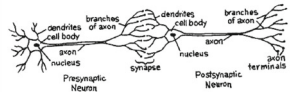
\includegraphics[width=\textwidth]{assets/pics/Aggarwal/Dendrit (Biological Neural Nework).png}
        \caption{Ilustrasi \textit{neural network} secara biologis
        \parencite{aggarwal2018neural}}
        \label{fig:biological_nn}
    \end{minipage}
    \hfill
    \begin{minipage}{0.48\textwidth}
        \centering
        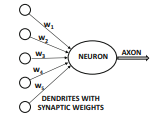
\includegraphics[width=\textwidth]{assets/pics/Aggarwal/NN ML.png}
        \caption{\textit{Artificial Neural Network} dengan representasi
        bobot sinapsis \parencite{aggarwal2018neural}}
        \label{fig:artificial_nn}
    \end{minipage}
\end{figure}

Dalam bentuk paling sederhananya, sebuah \textit{neural network} hanya
memiliki satu lapisan komputasi yang disebut \textit{perceptron}. Pada
arsitektur ini, terdapat $n$ neuron \textit{input} yang meneruskan fitur ke
satu neuron \textit{output} melalui sekumpulan bobot. Nilai \textit{output}
diperoleh dari penjumlahan bobot yang dikalikan dengan masing-masing nilai
\textit{input}, ditambah sebuah nilai \textit{bias} $b$ yang berfungsi
menggeser ambang batas keputusan model. Secara matematis, prediksi
\textit{output} dirumuskan sebagai:

\begin{equation}
    z = \mathbf{w} \cdot \mathbf{x} + b = \sum_{i=1}^{n} w_i x_i + b.
    \label{eq:perceptron}
\end{equation}

\noindent dengan $\mathbf{w}$ adalah vektor bobot, $\mathbf{x}$ adalah vektor
input, dan $b$ adalah skalar bias.

\textit{Perceptron} hanya mampu memodelkan hubungan linier antara
\textit{input} dan \textit{output}, sehingga tidak dapat menangani pola
yang lebih kompleks. Untuk mengatasi keterbatasan ini, digunakan
\textit{multilayer neural network} yang memiliki satu atau lebih
\textit{hidden layer} di antara \textit{input layer} dan \textit{output
layer}. Setiap lapisan menerima input dari lapisan sebelumnya dan
meneruskannya searah menuju \textit{output layer}. Pola aliran satu arah
seperti ini dikenal sebagai \textit{feed-forward}, dan arsitekturnya
ditunjukkan pada Gambar~\ref{fig:feedforward}.

\begin{figure}[H]
    \centering
    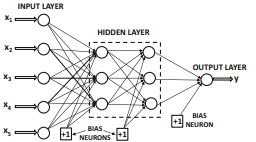
\includegraphics[width=0.7\textwidth]{assets/pics/Aggarwal/Multi Layer Bias.png}
    \caption{Arsitektur \textit{feed-forward neural network}
    \parencite{aggarwal2018neural}}
    \label{fig:feedforward}
\end{figure}

Misalkan terdapat $k$ \textit{hidden layer} dengan masing-masing $p_1,
\ldots, p_k$ neuron, $\mathbf{x}$ sebagai vektor input berisi $n$ neuron,
$\mathbf{h}_1, \ldots, \mathbf{h}_k$ sebagai keluaran tiap \textit{hidden
layer} setelah melewati fungsi aktivasi, dan $\mathbf{o}$ sebagai vektor
output berisi $m$ neuron. Matriks bobot $\mathbf{W}_1$ berdimensi
$n \times p_1$ menghubungkan \textit{input layer} dengan \textit{hidden
layer} pertama, $\mathbf{W}_r$ berdimensi $p_{r-1} \times p_r$
menghubungkan antar \textit{hidden layer}, dan $\mathbf{W}_{k+1}$
berdimensi $p_k \times m$ menghubungkan \textit{hidden layer} terakhir ke
\textit{output layer}. Proses komputasi pada tiap lapisan dirumuskan
sebagai:

\vspace{-1em}
\setlength{\abovedisplayskip}{0pt}
\begin{align}
    \mathbf{h}_1     &= \phi_1(\mathbf{W}_1^\top \mathbf{x}),
        \label{eq:input_to_hidden} \\
    \mathbf{h}_{r+1} &= \phi_{r+1}(\mathbf{W}_{r+1}^\top \mathbf{h}_r),
        \quad r \in \{1, \ldots, k-1\}, \label{eq:hidden_to_hidden} \\
    \mathbf{o}       &= \phi_0(\mathbf{W}_{k+1}^\top \mathbf{h}_k).
        \label{eq:hidden_to_output}
\end{align}

\noindent dengan $\phi_i$ adalah fungsi aktivasi yang diterapkan pada lapisan
ke-$i$. Output akhir $\mathbf{o}$ merupakan hasil transformasi bertingkat
dari input $\mathbf{x}$ melalui seluruh lapisan jaringan secara berurutan.

%-------------------------------------------------------------------------%
\subsection{Fungsi Aktivasi}
%-------------------------------------------------------------------------%

Fungsi aktivasi digunakan dalam \textit{neural network} untuk memberikan
sifat nonlinier pada model. Tanpa fungsi aktivasi, output jaringan hanya
merupakan transformasi linier dari input sehingga tidak mampu menangkap
pola yang kompleks \parencite{goodfellow2016}. Pada penelitian ini, digunakan tiga fungsi aktivasi utama,
yaitu \textit{softmax}, ReLU, dan GELU, yang masing-masing dijelaskan
berikut.

%-------------------------------------------------------------------------%
\subsubsection{\textit{Softmax}}
%-------------------------------------------------------------------------%

Fungsi \textit{softmax} digunakan untuk mengubah vektor bernilai real menjadi 
distribusi probabilitas pada $K$ kelas. Melalui proses ini, setiap nilai keluaran 
berada pada rentang 0 hingga 1, dengan total seluruh probabilitas sama dengan 1. 
Untuk vektor masukan $\mathbf{v} = (v_1, v_2, \ldots, v_K)$, fungsi \textit{softmax}
pada elemen ke-$j$ didefinisikan sebagai:

\vspace{-1em}
\setlength{\abovedisplayskip}{0pt}
\begin{equation}
    \phi(\mathbf{v})_j = \frac{e^{v_j}}{\displaystyle\sum_{k=1}^{K} e^{v_k}}.
    \label{eq:softmax}
\end{equation}

\noindent dengan $e$ adalah bilangan Euler bernilai sekitar $2{,}718$. Elemen dengan nilai $v_j$ 
yang lebih besar menghasilkan $e^{v_j}$ yang
lebih besar, sehingga probabilitas $\phi(\mathbf{v})_j$ yang diperoleh
juga lebih tinggi. Fungsi \textit{softmax} umum digunakan pada
lapisan keluaran jaringan untuk tugas klasifikasi multikelas karena
keluarannya dapat langsung diinterpretasikan sebagai probabilitas prediksi
tiap kelas.

%-------------------------------------------------------------------------%
\subsubsection{\textit{Rectified Linear Unit} (ReLU)}
%-------------------------------------------------------------------------%

\textit{Rectified Linear Unit} (ReLU) mengatasi masalah \textit{vanishing
gradient} dengan cara meneruskan nilai \textit{input} apa adanya jika
positif, dan mengembalikan nol jika negatif:

\vspace{-1em}
\setlength{\abovedisplayskip}{0pt}
\begin{equation}
    \phi(v) = \max\{v,\, 0\}.
    \label{eq:relu}
\end{equation}

ReLU lebih efisien secara komputasi dan lebih mudah dilatih pada jaringan
yang dalam, karena gradiennya selalu bernilai 1 untuk \textit{input}
positif sehingga informasi pembaruan tidak melemah saat merambat mundur
melalui banyak lapisan.

%-------------------------------------------------------------------------%
\subsubsection{\textit{Gaussian Error Linear Unit} (GELU)}
%-------------------------------------------------------------------------%

\textit{Gaussian Error Linear Unit} (GELU) digunakan sebagai 
fungsi aktivasi pada arsitektur \textit{Transformer} seperti BERT \parencite{hendrycks2016}. Berbeda dengan ReLU 
yang mengubah seluruh nilai negatif menjadi nol, GELU mengatur kontribusi 
setiap nilai \textit{input} berdasarkan probabilitas kumulatif distribusi 
Gaussian pada nilai tersebut:

\vspace{-1em}
\setlength{\abovedisplayskip}{0pt}
\begin{equation}
    \phi(v) = v \cdot \Phi(v) = v \cdot \frac{1}{2}\left[1 +
    \operatorname{erf}\!\left(\frac{v}{\sqrt{2}}\right)\right].
    \label{eq:gelu}
\end{equation}

\noindent dengan $\Phi(v)$ adalah fungsi distribusi kumulatif Gaussian standar,
dan $\operatorname{erf}(\cdot)$ adalah fungsi error dengan rentang nilai
$[-1, 1]$, sehingga $\Phi(v) \in [0, 1]$. Untuk $v$ besar dan positif,
GELU mendekati perilaku ReLU, sedangkan di sekitar nol transisinya
berlangsung mulus.

\begin{figure}[H]
    \centering
    \resizebox{\textwidth}{!}{%
        \begin{tabular}{ccc}
            \actplot{Softmax (2 kelas)}{%
                \addplot[teal, ultra thick] {exp(x)/(exp(x)+exp(-x))};
                \addplot[dashed, gray!60] coordinates {(-4.2,1)(4.2,1)};
            }{-0.2}{1.3}
            &
            \actplot{ReLU}{%
                \addplot[red!75!black, ultra thick] {max(x,0)};
            }{-0.8}{4.5}
            &
            \actplot{GELU}{%
                \addplot[blue!70!black, ultra thick]
                    {x * (1 + tanh(sqrt(2/pi) * (x + 0.044715 * x^3))) / 2};
            }{-0.8}{4.5}
        \end{tabular}%
    }
    \caption{Grafik fungsi aktivasi: \textit{Softmax}, ReLU, dan GELU}
    \label{fig:activation_functions}
\end{figure}

Perbandingan ketiga fungsi aktivasi ditunjukkan pada
Gambar~\ref{fig:activation_functions}.

%-------------------------------------------------------------------------%
\subsection{Fungsi \textit{Loss}}
%-------------------------------------------------------------------------%

Fungsi \textit{loss} mengukur seberapa jauh prediksi model menyimpang dari
nilai yang sebenarnya. Untuk tugas klasifikasi multikelas,
\textit{categorical cross-entropy loss} merupakan pilihan yang umum
digunakan \parencite{aggarwal2018neural}:

\begin{equation}
    L = -\sum_{i=1}^{n} \sum_{j=1}^{k} y_{ij} \log(\hat{y}_{ij}).
    \label{eq:categorical_crossentropy}
\end{equation}

\noindent dengan $n$ adalah jumlah sampel, $k$ adalah jumlah kelas, $y_{ij}$
adalah label aktual dalam bentuk \textit{one-hot encoded} bernilai 1
jika sampel ke-$i$ termasuk kelas ke-$j$ dan 0 jika tidak, serta
$\hat{y}_{ij}$ adalah probabilitas prediksi model untuk sampel ke-$i$
pada kelas ke-$j$.

%-------------------------------------------------------------------------%
\subsection{\textit{Backpropagation}}
%-------------------------------------------------------------------------%

Setelah nilai \textit{loss} diperoleh, langkah berikutnya dalam proses
pelatihan adalah menghitung gradien terhadap parameter model untuk
menentukan arah pembaruan bobot. Proses tersebut dilakukan menggunakan
algoritma \textit{backpropagation}
\parencite{aggarwal2018neural}.

\textit{Backpropagation} bekerja dengan merambatkan informasi kesalahan
dari lapisan keluaran menuju lapisan sebelumnya untuk menghitung seberapa
besar kontribusi masing-masing parameter terhadap nilai
\textit{loss}. Perhitungan tersebut dilakukan menggunakan aturan rantai
(\textit{chain rule}), karena keluaran model umumnya diperoleh melalui
serangkaian fungsi yang saling bergantung.

Hubungan tersebut dapat dijelaskan menggunakan graf komputasi pada
Gambar~\ref{fig:backprop_structure}.

\begin{figure}[H]
\centering
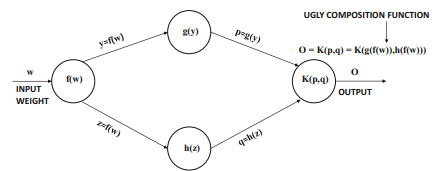
\includegraphics[width=0.6\textwidth]
{assets/pics/Aggarwal/NN Backprop.png}
\caption{Ilustrasi graf komputasi pada proses
\textit{backpropagation}
\parencite{aggarwal2018neural}}
\label{fig:backprop_structure}
\end{figure}

Pada Gambar~\ref{fig:backprop_structure}, parameter $w$ diproses melalui
beberapa tahapan transformasi hingga menghasilkan keluaran akhir $o$.
Keluaran tersebut diperoleh dari dua jalur komputasi yang digabungkan
melalui fungsi:

\begin{equation}
o
=
K(g(f(w)),h(f(w)))
\label{eq:output_composite}
\end{equation}

Persamaan~\ref{eq:output_composite} menunjukkan bahwa keluaran merupakan
fungsi komposit terhadap parameter $w$. Oleh karena itu, pengaruh perubahan
parameter terhadap nilai \textit{loss} dihitung menggunakan aturan rantai
sebagai berikut:

\begin{equation}
\frac{\partial L}{\partial w}
=
\frac{\partial L}{\partial o}
\left(
\frac{\partial o}{\partial p}
\cdot
\frac{\partial p}{\partial y}
\cdot
\frac{\partial y}{\partial w}
+
\frac{\partial o}{\partial q}
\cdot
\frac{\partial q}{\partial z}
\cdot
\frac{\partial z}{\partial w}
\right)
\label{eq:backprop_chain_rule}
\end{equation}

Pada Persamaan~\ref{eq:backprop_chain_rule},
$\partial L/\partial o$ menyatakan perubahan nilai
\textit{loss} terhadap perubahan keluaran model, sedangkan suku di dalam
tanda kurung menyatakan pengaruh parameter terhadap keluaran melalui
masing-masing jalur komputasi. Gradien diperoleh dengan mengalikan turunan
lokal pada setiap tahapan transformasi dan menjumlahkan kontribusi dari
seluruh jalur yang memengaruhi keluaran.

Proses penyebaran gradien dari keluaran menuju parameter pada tahapan
komputasi sebelumnya inilah yang disebut sebagai
\textit{backpropagation}.


%-------------------------------------------------------------------------%
\subsection{Teknik Optimasi}
%-------------------------------------------------------------------------%

Proses optimasi merupakan tahapan pencarian parameter yang menghasilkan
nilai fungsi \textit{loss} sekecil mungkin selama pelatihan
\parencite{zhang2023}. Gradien yang diperoleh dari \textit{backpropagation}
digunakan untuk memperbarui bobot model secara iteratif.

%-------------------------------------------------------------------------%
\subsubsection{\textit{Stochastic Gradient Descent} (SGD)}
%-------------------------------------------------------------------------%

\textit{Stochastic Gradient Descent} (SGD) adalah algoritma optimasi yang
diperkenalkan oleh \parencite{rumelhart1986} untuk meminimalkan fungsi
\textit{loss} $L(\mathbf{w})$ secara iteratif dengan memperbarui bobot
ke arah negatif gradiennya:

\vspace{-1em}
\setlength{\abovedisplayskip}{0pt}
\begin{equation}
    \mathbf{w}^{[t+1]} = \mathbf{w}^{[t]} - \eta \nabla L(\mathbf{w})^{[t]}.
    \label{eq:sgd}
\end{equation}

\noindent dengan $\mathbf{w}^{[t]}$ adalah vektor bobot pada iterasi ke-$t$,
$\nabla L(\mathbf{w})^{[t]}$ adalah vektor gradien fungsi \textit{loss}
terhadap bobot pada iterasi ke-$t$, dan $\eta$ adalah skalar
\textit{learning rate} yang mengontrol besar langkah pembaruan. Nilai
$\eta$ yang terlalu kecil memperlambat konvergensi, sedangkan nilai yang
terlalu besar dapat membuat pelatihan tidak stabil.

%-------------------------------------------------------------------------%
\subsubsection{\textit{Adaptive Moment Estimation} (Adam)}
%-------------------------------------------------------------------------%

\textit{Adaptive Moment Estimation} (Adam), yang dikemukakan oleh
\parencite{kingma2017}, mengembangkan SGD dengan mengadaptasi
\textit{learning rate} secara individual untuk setiap parameter. Adaptasi
ini didasarkan pada dua estimasi momen gradien: momen pertama
$\mathbf{v}^{[t]}$ terhadap gradien itu sendiri, dan momen kedua
$\mathbf{s}^{[t]}$ terhadap kuadrat gradien:

\vspace{-1em}
\setlength{\abovedisplayskip}{0pt}
\begin{equation}
    \mathbf{v}^{[t]} = \beta_1 \mathbf{v}^{[t-1]}
    + (1 - \beta_1) \nabla L(\mathbf{w})^{[t]}.
    \label{eq:adam_first_moment}
\end{equation}
\begin{equation}
    \mathbf{s}^{[t]} = \beta_2 \mathbf{s}^{[t-1]}
    + (1 - \beta_2) \left(\nabla L(\mathbf{w})^{[t]}\right)^2.
    \label{eq:adam_second_moment}
\end{equation}

\noindent dengan $\beta_1$ dan $\beta_2$ adalah skalar koefisien peluruhan yang
mengontrol pengaruh gradien lama terhadap estimasi saat ini. Karena kedua
momen diinisialisasi dengan nol, estimasinya cenderung bias ke nol pada
iterasi awal. Koreksi bias dilakukan dengan normalisasi:

\vspace{-1em}
\setlength{\abovedisplayskip}{0pt}
\begin{equation}
    \hat{\mathbf{v}}^{[t]} = \frac{\mathbf{v}^{[t]}}{1 - \beta_1^t},
    \qquad
    \hat{\mathbf{s}}^{[t]} = \frac{\mathbf{s}^{[t]}}{1 - \beta_2^t}.
    \label{eq:adam_bias_correction}
\end{equation}

Seiring bertambahnya $t$, nilai $\beta_1^t$ dan $\beta_2^t$ mendekati nol
sehingga koreksi ini semakin tidak berpengaruh. Pembaruan bobot dilakukan
menggunakan kedua momen yang telah dikoreksi:

\vspace{-1em}
\setlength{\abovedisplayskip}{0pt}
\begin{equation}
    \mathbf{w}^{[t+1]} = \mathbf{w}^{[t]}
    - \frac{\eta}{\sqrt{\hat{\mathbf{s}}^{[t]}} + \epsilon}\,
    \hat{\mathbf{v}}^{[t]}.
    \label{eq:adam_update}
\end{equation}

\noindent dengan $\epsilon = 10^{-8}$ adalah skalar untuk mencegah pembagian
dengan nol \parencite{zhang2023}. Pembagian dengan
$\sqrt{\hat{\mathbf{s}}^{[t]}}$ memperkecil langkah pembaruan untuk
parameter dengan gradien besar dan berfluktuasi, serta memperbesar untuk
parameter dengan gradien kecil dan konsisten.

%-------------------------------------------------------------------------%
\subsection{Regularisasi}
%-------------------------------------------------------------------------%

Dalam melatih model, terdapat dua kondisi yang perlu dihindari, yaitu
\textit{underfitting} dan \textit{overfitting}.
\textit{Underfitting} terjadi ketika model gagal mempelajari pola data
pelatihan, ditandai dengan bias yang tinggi. \textit{Overfitting} terjadi
ketika model terlalu menghafalkan data pelatihan sehingga performanya
menurun pada data baru, ditandai dengan variansi yang tinggi
\parencite{goodfellow2016}.

Gambar~\ref{fig:underfitting_overfitting} menunjukkan hubungan antara
kompleksitas model dengan bias, variansi, dan total error. Bias menurun
seiring meningkatnya kompleksitas model, sementara variansi justru
meningkat. Total error yang merupakan kombinasi keduanya mencapai nilai
minimum pada titik kompleksitas optimal.

\begin{figure}[H]
    \centering
    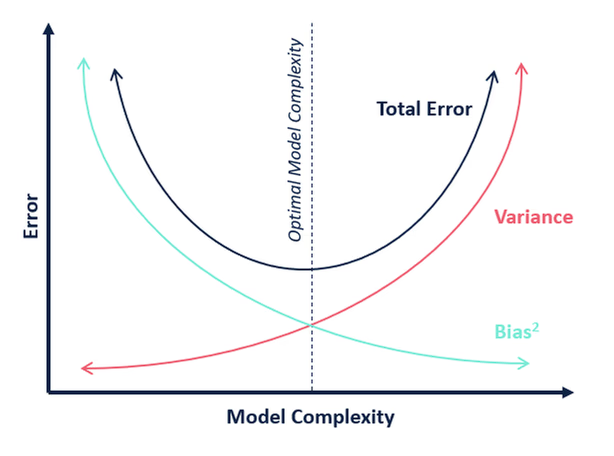
\includegraphics[width=0.6\textwidth]{assets/pics/Aggarwal/NN Regularization.png}
    \caption{Ilustrasi \textit{bias-variance tradeoff} terhadap kompleksitas
    model (\cite{aggarwal2018neural}, telah diolah kembali)}
    \label{fig:underfitting_overfitting}
\end{figure}

Untuk mencegah \textit{overfitting}, salah satu teknik yang digunakan
adalah \textit{weight decay} atau $L_2$ \textit{regularization}, yang
menambahkan penalti pada fungsi \textit{loss} proporsional terhadap besar
bobot model:

\begin{equation}
    \tilde{L}(\mathbf{w}) = L(\mathbf{w}) + \frac{\lambda}{2}
    \|\mathbf{w}\|^2.
    \label{eq:l2_regularization}
\end{equation}

\noindent dengan $L(\mathbf{w})$ adalah fungsi \textit{loss} asal,
$\|\mathbf{w}\|^2$ adalah jumlah kuadrat seluruh bobot dalam model, dan
$\lambda$ adalah skalar yang mengontrol kekuatan penalti.

Teknik lain yang digunakan adalah \textit{dropout}, yang menonaktifkan
neuron secara acak selama pelatihan agar jaringan tidak terlalu
bergantung pada neuron tertentu \parencite{srivastava2014dropout}. Untuk
vektor aktivasi $\mathbf{h} \in \mathbb{R}^p$, setiap neuron ke-$i$
dikalikan dengan variabel acak Bernoulli:

\begin{equation}
    m_i \sim \text{Bernoulli}(1 - p_{\text{drop}}), \qquad
    \tilde{h}_i = \frac{m_i}{1 - p_{\text{drop}}} \cdot h_i.
    \label{eq:dropout}
\end{equation}

\noindent dengan $p_{\text{drop}} \in [0,1]$ adalah probabilitas neuron
dinonaktifkan, dan faktor $1/(1-p_{\text{drop}})$ menyeimbangkan skala
aktivasi akibat neuron yang dinonaktifkan. Pada tahap evaluasi,
\textit{dropout} tidak diterapkan dan seluruh neuron digunakan
sepenuhnya ($\tilde{\mathbf{h}} = \mathbf{h}$).

Teknik lain yang juga memberikan efek regularisasi adalah \textit{Batch
Normalization} (BatchNorm), yang menormalisasi aktivasi berdasarkan
statistik \textit{mini-batch} untuk mempercepat dan menstabilkan
pelatihan \parencite{ioffe2015batch}. Untuk aktivasi
$\mathcal{B} = \{h_1, \ldots, h_m\}$ pada satu \textit{mini-batch}:

\begin{equation}
    \hat{h}_i = \frac{h_i - \mu_{\mathcal{B}}}
    {\sqrt{\sigma_{\mathcal{B}}^2 + \epsilon}}, \qquad
    \text{BN}(h_i) = \gamma \hat{h}_i + \beta.
    \label{eq:batchnorm}
\end{equation}

\noindent dengan $\mu_{\mathcal{B}}$ dan $\sigma_{\mathcal{B}}^2$
masing-masing adalah rata-rata dan variansi \textit{batch}, $\epsilon$
adalah skalar kecil pencegah pembagian dengan nol, serta $\gamma$ dan
$\beta$ adalah parameter skala dan pergeseran yang dipelajari agar
kapasitas representasi jaringan tetap terjaga. Pada tahap evaluasi,
$\mu_{\mathcal{B}}$ dan $\sigma_{\mathcal{B}}^2$ digantikan dengan
estimasi rata-rata bergerak yang dikumpulkan selama pelatihan.

%-------------------------------------------------------------------------%
\subsection{Metrik Evaluasi}
%-------------------------------------------------------------------------%

Tahap evaluasi bertujuan untuk mengukur kinerja model pada tugas
klasifikasi sentimen maupun klasterisasi topik. Evaluasi klasifikasi
dilakukan menggunakan metrik yang diturunkan dari
\textit{confusion matrix}, sedangkan evaluasi hasil klasterisasi topik
dilakukan menggunakan metrik \textit{topic coherence} dan
\textit{topic diversity}. Masing-masing metrik dijelaskan pada
subsubbab berikut.

%-------------------------------------------------------------------------%
\subsubsection{Metrik Evaluasi Klasifikasi}
%-------------------------------------------------------------------------%

Setelah model dilatih, performa klasifikasi dievaluasi menggunakan data
yang tidak digunakan selama proses pelatihan. Evaluasi didasarkan pada
\textit{confusion matrix}, yaitu tabel yang membandingkan hasil prediksi
model dengan label aktual. Dari tabel tersebut diperoleh empat komponen
dasar, yaitu \textit{True Positive} (TP), \textit{True Negative} (TN),
\textit{False Positive} (FP), dan \textit{False Negative} (FN). TP
menunjukkan jumlah sampel positif yang diprediksi dengan benar, TN
menunjukkan jumlah sampel negatif yang diprediksi dengan benar, FP
menunjukkan jumlah sampel negatif yang salah diprediksi sebagai positif,
sedangkan FN menunjukkan jumlah sampel positif yang salah diprediksi
sebagai negatif.

Berdasarkan keempat komponen tersebut, digunakan empat metrik evaluasi
utama, yaitu akurasi, \textit{precision}, \textit{recall}, dan
F1-\textit{Score}.

Akurasi mengukur proporsi keseluruhan prediksi yang benar terhadap seluruh
sampel pengujian.

\begin{equation}
    \text{Accuracy} =
    \frac{TP + TN}{TP + TN + FP + FN}
    \label{eq:accuracy}
\end{equation}

\textit{Precision} mengukur ketepatan model ketika memprediksi suatu
sampel sebagai kelas positif, yaitu proporsi prediksi positif yang benar.

\begin{equation}
    \text{Precision} =
    \frac{TP}{TP + FP}
    \label{eq:precision}
\end{equation}

\textit{Recall} mengukur kemampuan model dalam menemukan seluruh sampel
positif yang sebenarnya.

\begin{equation}
    \text{Recall} =
    \frac{TP}{TP + FN}
    \label{eq:recall}
\end{equation}

Karena \textit{precision} dan \textit{recall} sering kali saling
berkompromi, keduanya dikombinasikan menggunakan F1-\textit{Score},
yaitu rata-rata harmonik antara kedua metrik tersebut.

\begin{equation}
    \text{F1-Score}
    =
    2
    \times
    \frac{\text{Precision} \times \text{Recall}}
    {\text{Precision} + \text{Recall}}
    =
    \frac{2TP}{2TP + FP + FN}
    \label{eq:f1score}
\end{equation}

F1-\textit{Score} memberikan ukuran yang lebih seimbang dibandingkan
akurasi, terutama pada dataset yang memiliki distribusi kelas tidak
seimbang.

%-------------------------------------------------------------------------%
\subsubsection{Metrik Evaluasi Topik}
\label{sec:topic_eval}
%-------------------------------------------------------------------------%

Kualitas hasil klasterisasi topik dapat dievaluasi menggunakan berbagai
metrik kuantitatif. Pada penelitian ini digunakan dua metrik, yaitu
\textit{topic coherence} dan \textit{topic diversity}. Kedua metrik
dihitung langsung dari dokumen hasil klasterisasi tanpa memerlukan model
eksternal.

\textit{Topic coherence} mengukur sejauh mana kata-kata teratas dalam
suatu topik memiliki keterkaitan semantik melalui kemunculan bersama
(\textit{co-occurrence}) pada dokumen yang sama. Penelitian ini
menggunakan metrik \textit{Normalized Pointwise Mutual Information}
(NPMI). Misalkan $\mathcal{D}_k$ adalah himpunan dokumen pada klaster
ke-$k$ dan $\{w_1,w_2,\ldots,w_N\}$ merupakan $N$ kata teratas pada
klaster tersebut setelah proses penghapusan \textit{stop words}.
Probabilitas kemunculan setiap kata dan probabilitas kemunculan
bersamanya didefinisikan sebagai

\begin{align}
    p(w_i)
    &= \frac{|\{d \in \mathcal{D}_k : w_i \in d\}|}
    {|\mathcal{D}_k|},\\[4pt]
    p(w_j)
    &= \frac{|\{d \in \mathcal{D}_k : w_j \in d\}|}
    {|\mathcal{D}_k|},\\[4pt]
    p(w_i,w_j)
    &= \frac{|\{d \in \mathcal{D}_k :
    w_i \in d \text{ dan } w_j \in d\}|}
    {|\mathcal{D}_k|}.
\end{align}

Nilai \textit{Pointwise Mutual Information} (PMI) dihitung sebagai

\begin{equation}
    \mathrm{PMI}(w_i,w_j)
    =
    \log
    \frac{p(w_i,w_j)+\varepsilon}
    {p(w_i)p(w_j)+\varepsilon}
    \label{eq:pmi}
\end{equation}

dengan $\varepsilon = 10^{-10}$ digunakan untuk menghindari pembagian
dengan nol. Selanjutnya nilai PMI dinormalisasi menjadi NPMI.

\begin{equation}
    \mathrm{NPMI}(w_i,w_j)
    =
    \frac{\mathrm{PMI}(w_i,w_j)}
    {-\log(p(w_i,w_j)+\varepsilon)}
    \label{eq:npmi}
\end{equation}

Nilai NPMI berada pada rentang $[-1,1]$, di mana nilai yang semakin
mendekati $1$ menunjukkan bahwa kedua kata semakin sering muncul
bersama. Skor \textit{topic coherence} untuk setiap klaster dihitung
sebagai rata-rata nilai NPMI seluruh pasangan kata.

\begin{equation}
    \mathrm{TC}_k
    =
    \frac{1}{\binom{N}{2}}
    \sum_{j=2}^{N}
    \sum_{i=1}^{j-1}
    \mathrm{NPMI}(w_i,w_j)
    \label{eq:tc_cluster}
\end{equation}

Nilai koherensi keseluruhan diperoleh melalui rata-rata seluruh klaster.

\begin{equation}
    \overline{\mathrm{TC}}
    =
    \frac{1}{K}
    \sum_{k=1}^{K}
    \mathrm{TC}_k
    \label{eq:tc_mean}
\end{equation}

Apabila suatu klaster memiliki kurang dari dua kata unik, maka nilai
koherensinya ditetapkan sebesar $0$.

\textit{Topic diversity} mengukur tingkat keberagaman kosakata antar
topik. Semakin sedikit kata yang muncul berulang pada topik berbeda,
semakin tinggi nilai \textit{topic diversity}. Misalkan $\mathcal{W}_k$
adalah himpunan $N$ kata teratas pada klaster ke-$k$, sedangkan himpunan
seluruh kata unik didefinisikan sebagai

\[
\mathcal{U}
=
\bigcup_{k=1}^{K}\mathcal{W}_k.
\]

Nilai \textit{topic diversity} dihitung menggunakan

\begin{equation}
    \mathrm{TD}
    =
    \frac{|\mathcal{U}|}
    {\displaystyle\sum_{k=1}^{K}|\mathcal{W}_k|}
    \label{eq:td}
\end{equation}

Nilai $\mathrm{TD}=1$ menunjukkan bahwa seluruh kata teratas dari setiap
topik berbeda satu sama lain, sedangkan nilai yang semakin kecil
menunjukkan semakin banyak kosakata yang tumpang tindih antar topik.

%-------------------------------------------------------------------------%
\section{\textit{Autoencoder}}
%-------------------------------------------------------------------------%

Pemahaman tentang arsitektur \textit{feed-forward neural network} menjadi
landasan untuk memahami \textit{autoencoder}, yang pada dasarnya adalah
sebuah jaringan saraf yang dilatih untuk merekonstruksi inputnya
\parencite{goodfellow2016}. Karena tidak memerlukan label,
\textit{autoencoder} termasuk ke dalam kategori \textit{unsupervised
learning} \parencite{hinton2006reducing}.

Arsitektur \textit{autoencoder} \parencite{vincent2010stacked} terdiri
dari dua komponen utama: \textit{encoder} yang memetakan representasi
input dari dimensi tinggi ke dimensi yang lebih rendah, dan
\textit{decoder} yang merekonstruksi representasi tersebut ke dimensi
semula. Lapisan tersempit di antara keduanya disebut \textit{bottleneck}
atau ruang laten. Arsitektur lengkapnya ditunjukkan pada
Gambar~\ref{fig:autoencoder_architecture}.

\begin{figure}[H]
    \centering
    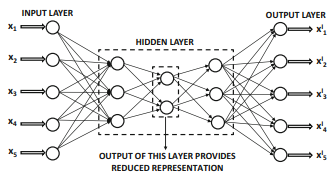
\includegraphics[width=0.75\textwidth]{assets/pics/Aggarwal/Autoencoder.png}
    \caption{Arsitektur \textit{autoencoder} menunjukkan proses
    \textit{encoding} dan \textit{decoding} \parencite{aggarwal2018neural}}
    \label{fig:autoencoder_architecture}
\end{figure}

%-------------------------------------------------------------------------%
\subsection{\textit{Encoder} dan \textit{Decoder}}
%-------------------------------------------------------------------------%

Secara formal, misalkan $\mathbf{x} \in \mathbb{R}^D$ adalah vektor input
berdimensi $D$. \textit{Encoder} memetakan $\mathbf{x}$ ke dalam vektor
laten $\mathbf{z} \in \mathbb{R}^d$ dengan $d < D$:

\begin{equation}
    \mathbf{z} = f_\theta(\mathbf{x}) =
    \sigma_h(\mathbf{W}_h \mathbf{x} + \mathbf{b}_h).
    \label{eq:encoder}
\end{equation}

\noindent dengan $\mathbf{W}_h \in \mathbb{R}^{d \times D}$ adalah matriks bobot
\textit{encoder}, $\mathbf{b}_h \in \mathbb{R}^d$ adalah vektor bias, dan
$\sigma_h(\cdot)$ adalah fungsi aktivasi. Simbol $\theta$
merepresentasikan seluruh parameter pada bagian \textit{encoder}.

Selanjutnya, \textit{decoder} memetakan kembali vektor laten $\mathbf{z}$
ke dalam ruang dimensi asal untuk menghasilkan rekonstruksi
$\hat{\mathbf{x}} \in \mathbb{R}^D$:

\begin{equation}
    \hat{\mathbf{x}} = g_{\theta'}(\mathbf{z}) =
    \sigma_o(\mathbf{W}_o \mathbf{z} + \mathbf{b}_o).
    \label{eq:decoder}
\end{equation}

\noindent dengan $\mathbf{W}_o \in \mathbb{R}^{D \times d}$ adalah matriks bobot
\textit{decoder}, $\mathbf{b}_o \in \mathbb{R}^D$ adalah vektor bias, dan
$\sigma_o(\cdot)$ adalah fungsi aktivasi output. Simbol $\theta'$
merepresentasikan seluruh parameter pada bagian \textit{decoder}. Secara
keseluruhan, \textit{autoencoder} melakukan transformasi:

\begin{equation}
    \hat{\mathbf{x}} = g_{\theta'}(f_\theta(\mathbf{x})).
    \label{eq:autoencoder_full}
\end{equation}

%-------------------------------------------------------------------------%
\subsection{Fungsi Objektif}
%-------------------------------------------------------------------------%

\textit{Autoencoder} dilatih dengan meminimalkan selisih antara
\textit{input} asal dan hasil rekonstruksinya. Pada penelitian ini,
fungsi \textit{loss} yang digunakan adalah \textit{Mean Squared Error}
(MSE):

\begin{equation}
    \mathcal{L}(\theta, \theta') = \frac{1}{n} \sum_{i=1}^{n}
    \|\mathbf{x}_i - g_{\theta'}(f_\theta(\mathbf{x}_i))\|^2.
    \label{eq:reconstruction_loss}
\end{equation}

\noindent dengan $n$ adalah jumlah sampel dan $\|\cdot\|^2$ adalah kuadrat norma
Euclidean. Parameter \textit{encoder} $\theta$ dan \textit{decoder}
$\theta'$ diperbarui secara bersama-sama menggunakan
\textit{backpropagation} dan optimasi Adam \parencite{vincent2010stacked}.

%-------------------------------------------------------------------------%
\section{Bidirectional Encoder Representations from Transformers (BERT)}
\label{sec:bert}
%-------------------------------------------------------------------------%

\textit{Bidirectional Encoder Representations from Transformers} (BERT) merupakan model bahasa berbasis \textit{Transformer} yang diperkenalkan oleh \parencite{devlin2018bert}. Berbeda dengan pendekatan sebelumnya yang umumnya memodelkan bahasa secara satu arah, BERT menghasilkan representasi kontekstual dua arah dengan memanfaatkan mekanisme \textit{self-attention}. Melalui mekanisme tersebut, setiap token dapat memperhatikan informasi dari token lain dalam urutan teks, baik yang berada di sisi kiri maupun kanan.

BERT dilatih menggunakan korpus Wikipedia bahasa Inggris dan BookCorpus melalui dua tugas pra-pelatihan, yaitu \textit{Masked Language Modeling} (MLM) dan \textit{Next Sentence Prediction} (NSP). Pada penelitian ini, model BERT hasil pra-pelatihan digunakan tanpa proses \textit{fine-tuning}. Seluruh parameter BERT dipertahankan tetap (\textit{frozen}), sehingga keluaran representasinya digunakan secara langsung sebagai fitur numerik untuk tahap pemodelan berikutnya.

%-------------------------------------------------------------------------%
\subsection{Representasi Input BERT}
\label{subsec:bert_input}
%-------------------------------------------------------------------------%

Setiap token hasil tokenisasi pada input BERT terlebih dahulu diubah menjadi vektor numerik. Representasi awal setiap token diperoleh dari penjumlahan tiga komponen \textit{embedding}, yaitu:

\begin{equation}
\mathbf{E}_i = \mathbf{E}_{\text{token}}^{(i)} + \mathbf{E}_{\text{segment}}^{(i)} + \mathbf{E}_{\text{position}}^{(i)}.
\end{equation}

Komponen pertama, \textit{token embedding}, memberikan representasi semantik dari token atau \textit{subword} yang diperoleh melalui proses tokenisasi WordPiece. Komponen kedua, \textit{segment embedding}, memberikan informasi mengenai segmen atau pasangan kalimat tempat suatu token berada dan terutama digunakan ketika \textit{input} terdiri dari dua kalimat. Sementara itu, \textit{position embedding} memberikan informasi mengenai posisi token dalam urutan teks. Berbeda dengan Transformer awal yang menggunakan fungsi sinusoidal untuk menentukan posisi token, BERT mempelajari parameter posisi tersebut secara langsung selama proses pra-pelatihan.

\begin{figure}[H]
\centering
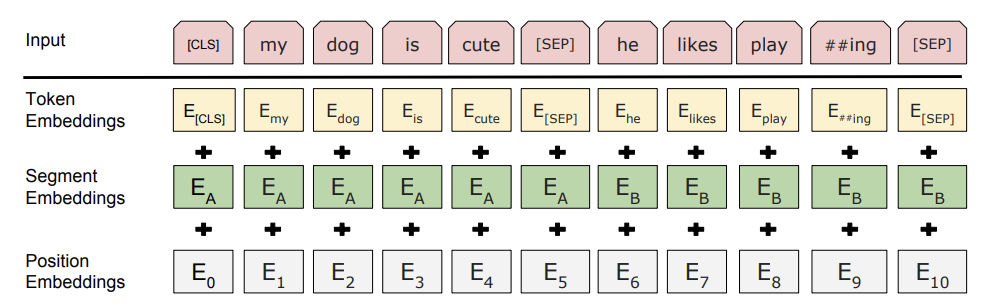
\includegraphics[width=0.9\textwidth]{assets/pics/BERT/bert_representation.png}
\caption{Representasi \textit{input} BERT yang terdiri dari \textit{token}, \textit{segment}, dan \textit{position embedding} \parencite{devlin2018bert}}
\label{fig:bert_input}
\end{figure}

Selain token hasil tokenisasi, BERT menambahkan token khusus \texttt{[CLS]} pada awal urutan \textit{input}. Representasi token tersebut kemudian diproses bersama token lainnya melalui seluruh lapisan \textit{Transformer Encoder} sehingga dapat digunakan sebagai representasi agregat dari urutan teks. Gabungan seluruh vektor $\mathbf{E}_i$ menjadi masukan awal bagi tumpukan \textit{Transformer Encoder}:

\begin{equation}
\mathbf{H}^{(0)} = \mathbf{E} = [\mathbf{E}_{[\text{CLS}]}, \mathbf{E}_1, \mathbf{E}_2, \ldots, \mathbf{E}_n].
\end{equation}

%-------------------------------------------------------------------------%
\subsection{Arsitektur BERT}
\label{subsec:bert_arch}
%-------------------------------------------------------------------------%

Representasi awal $\mathbf{H}^{(0)}$ dilewatkan melalui $L$ lapisan \textit{Transformer Encoder} yang memiliki struktur identik (Gambar~\ref{fig:bert_architecture}). Pada setiap lapisan, representasi tersebut diperbarui melalui mekanisme \textit{self-attention} dan \textit{Position-wise Feed-Forward Network} (FFN), sehingga diperoleh urutan representasi:

\begin{equation}
\mathbf{H}^{(0)} \rightarrow \mathbf{H}^{(1)} \rightarrow \cdots \rightarrow \mathbf{H}^{(L)}.
\end{equation}

\begin{figure}[H]
\centering
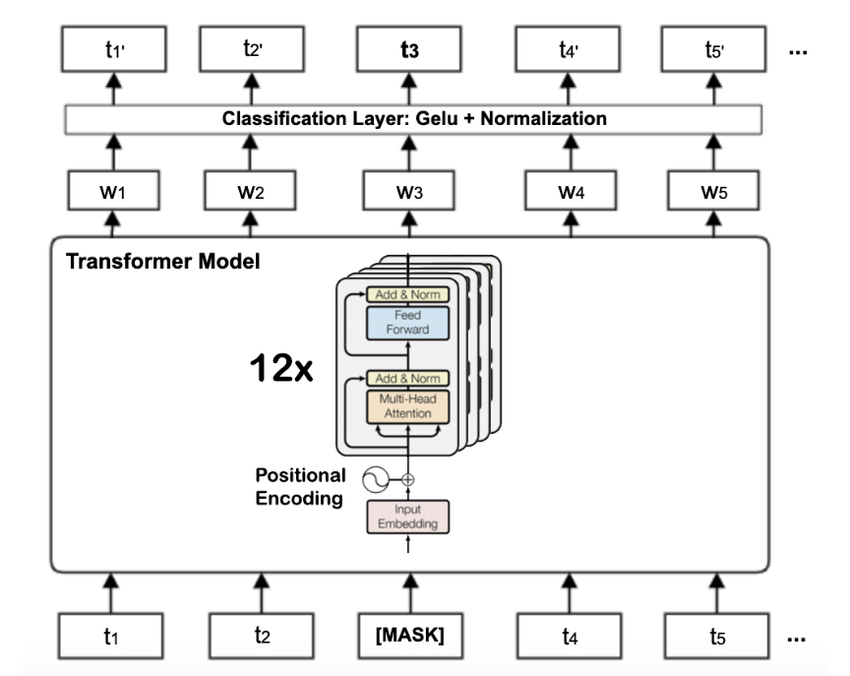
\includegraphics[width=0.6\textwidth]{assets/pics/BERT/Encoder_Stack_BERT.png}
\caption{Tumpukan $L$ lapisan \textit{Transformer Encoder} pada BERT \parencite{devlin2018bert}}
\label{fig:bert_architecture}
\end{figure}

Setiap lapisan \textit{Transformer Encoder} terdiri atas dua sub-lapisan utama, yaitu \textit{Multi-Head Self-Attention} dan \textit{Position-wise Feed-Forward Network} (FFN). Kedua sub-lapisan tersebut dilengkapi dengan koneksi residual dan normalisasi lapisan melalui mekanisme \textit{Add \& Norm} (Gambar~\ref{fig:bert_encoder_layer}). Secara matematis, keluaran dari setiap lapisan dihitung sebagai:

\begin{align}
\mathbf{H}^{(\ell)}_{\text{attn}} &= \text{LayerNorm}\!\left(\mathbf{H}^{(\ell-1)} + \text{MultiHeadAttention}(\mathbf{H}^{(\ell-1)})\right), \\
\mathbf{H}^{(\ell)} &= \text{LayerNorm}\!\left( \mathbf{H}^{(\ell)}_{\text{attn}} + \text{FFN}(\mathbf{H}^{(\ell)}_{\text{attn}})\right).
\end{align}

\begin{figure}[H]
\centering
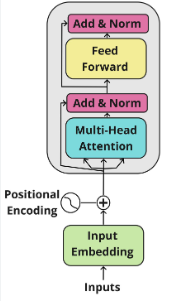
\includegraphics[width=0.3\textwidth]{assets/pics/BERT/Transfomer_Encoder_Layer.png}
\caption{Struktur satu lapisan \textit{Transformer Encoder} \parencite{devlin2018bert}}
\label{fig:bert_encoder_layer}
\end{figure}

Jumlah lapisan $L$, dimensi \textit{hidden state} $d$, dan jumlah \textit{attention head} $h$ bergantung pada varian BERT yang digunakan. Konfigurasi parameter BERT pada penelitian ini dijelaskan pada Bab Metodologi.

%-------------------------------------------------------------------------%
\subsection{Mekanisme \textit{Self-Attention}}
\label{subsec:bert_attention}
%-------------------------------------------------------------------------%

Mekanisme \textit{Multi-Head Self-Attention} memungkinkan setiap token memperhatikan token lain dalam suatu urutan berdasarkan tingkat relevansinya. \textit{Input} $\mathbf{H}^{(\ell-1)} \in \mathbb{R}^{n \times d}$ diproyeksikan menjadi tiga representasi, yaitu \textit{query} ($\mathbf{Q}$), \textit{key} ($\mathbf{K}$), dan \textit{value} ($\mathbf{V}$), melalui matriks bobot yang dipelajari selama proses pelatihan:

\begin{align}
\mathbf{Q} &= \mathbf{H}^{(\ell-1)}\mathbf{W}_Q \in \mathbb{R}^{n \times d_k}, \\
\mathbf{K} &= \mathbf{H}^{(\ell-1)}\mathbf{W}_K \in \mathbb{R}^{n \times d_k}, \\
\mathbf{V} &= \mathbf{H}^{(\ell-1)}\mathbf{W}_V \in \mathbb{R}^{n \times d_v}.
\end{align}

Dalam mekanisme ini, \textit{query} digunakan untuk menghitung tingkat kesesuaian dengan token lain, \textit{key} berfungsi sebagai representasi pembanding dalam perhitungan relevansi, sedangkan \textit{value} menyediakan informasi yang akan dikombinasikan berdasarkan bobot \textit{attention}. Skor relevansi antar-token diperoleh melalui perkalian $\mathbf{Q}\mathbf{K}^\top$, kemudian diskalakan dengan $\sqrt{d_k}$ dan dinormalisasi menggunakan fungsi \textit{softmax} untuk menghasilkan bobot \textit{attention}:

\begin{equation}
\text{Attention}(\mathbf{Q}, \mathbf{K}, \mathbf{V}) = \text{softmax}\!\left(\frac{\mathbf{Q}\mathbf{K}^\top}{\sqrt{d_k}} \right)\mathbf{V}.
\label{eq:attention}
\end{equation}

Untuk menangkap hubungan antar-token dari beberapa ruang representasi yang berbeda, BERT menggunakan beberapa \textit{attention head} yang bekerja secara paralel sebanyak $h$ buah (\textit{Multi-Head Attention}, Gambar~\ref{fig:multihead_attention}). Hasil dari setiap \textit{head} kemudian digabungkan dan diproyeksikan kembali ke dimensi semula:

\begin{equation}
\text{MultiHead}(\mathbf{Q}, \mathbf{K}, \mathbf{V}) = \text{Concat}(\text{head}_1, \ldots, \text{head}_h)\,\mathbf{W}_O.
\end{equation}

\noindent dengan $\text{head}_i = \text{Attention}(\mathbf{Q}\mathbf{W}_Q^i,\, \mathbf{K}\mathbf{W}_K^i,\, \mathbf{V}\mathbf{W}_V^i)$. Pada BERT-Base, jumlah \textit{attention head} yang digunakan adalah $h=12$ dengan dimensi masing-masing $\mathbf{Q}$ dan $\mathbf{K}$ sebesar $d_k=64$, serta $\mathbf{V}$ sebesar $d_v=64$.

\begin{figure}[H]
\centering
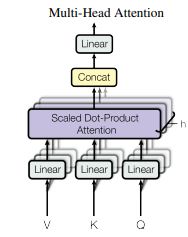
\includegraphics[width=0.3\textwidth]{assets/pics/BERT/transformer_attention.png}
\caption{Mekanisme \textit{Scaled Dot-Product Attention} pada \textit{Multi-Head Attention} \parencite{vaswani2017attention}}
\label{fig:multihead_attention}
\end{figure}

%-------------------------------------------------------------------------%
\subsection{Ekstraksi Fitur dari Token \texttt{[CLS]}}
\label{subsec:bert_feature}
%-------------------------------------------------------------------------%

Setelah melewati $L$ lapisan \textit{Transformer Encoder}, diperoleh \textit{hidden state} akhir $\mathbf{H}^{(L)}$ yang berisi representasi kontekstual dari seluruh token pada urutan input. Pada penelitian ini, representasi token \texttt{[CLS]} pada lapisan terakhir digunakan sebagai vektor fitur untuk setiap dokumen:

\begin{equation}
\mathbf{f} = \mathbf{H}^{(L)}_{[\text{CLS}]} \in \mathbb{R}^{d}.
\end{equation}

\noindent dengan $d$ merupakan dimensi \textit{hidden state} yang bergantung pada varian BERT yang digunakan. Token \texttt{[CLS]} dipilih karena representasinya telah diproses bersama seluruh token lainnya melalui mekanisme \textit{self-attention}, sehingga dapat digunakan sebagai representasi agregat dari suatu urutan teks. Karena parameter BERT dibekukan (\textit{frozen}) selama proses pelatihan, vektor fitur $\mathbf{f}$ diperoleh melalui proses \textit{forward pass} tanpa adanya pembaruan bobot. Selanjutnya, vektor tersebut digunakan sebagai masukan bagi \textit{autoencoder} untuk tahap reduksi dimensi.

%-------------------------------------------------------------------------%
\section{Multi-Task Learning}
%-------------------------------------------------------------------------%

\textit{Multi-Task Learning} (MTL) merupakan pendekatan dalam
\textit{machine learning} yang bertujuan meningkatkan kemampuan
generalisasi model dengan memanfaatkan informasi dari beberapa tugas yang
saling berkaitan secara bersamaan \parencite{caruana1997multitask}. Ketika
dua tugas memiliki keterkaitan, informasi pembelajaran dari satu tugas
dapat membantu tugas lainnya karena keduanya berbagi pola atau struktur
yang sama dalam data.

Konsep kunci yang mendasari MTL adalah \textit{inductive transfer}, yaitu
kemampuan model untuk memindahkan pengetahuan yang dipelajari dari satu
tugas ke tugas lainnya. \parencite{caruana1997multitask} menjelaskan bahwa
MTL mencapai hal ini dengan cara mempelajari beberapa tugas secara paralel
menggunakan representasi bersama. Tugas-tugas lain berfungsi sebagai
\textit{inductive bias}, yaitu mekanisme yang mengarahkan model agar
mempelajari hipotesis yang dapat menjelaskan lebih dari satu tugas
sekaligus \parencite{ruder2017overview}.

Pada penelitian ini, MTL digunakan untuk mempelajari analisis sentimen dan
pendeteksian topik secara bersamaan. Kedua tugas ini memiliki keterkaitan
yang kuat karena sama-sama bergantung pada pemahaman semantis teks ulasan,
sehingga representasi yang berguna untuk mendeteksi topik juga cenderung
berguna untuk mengklasifikasikan sentimen.

%-------------------------------------------------------------------------%
\subsection{Formulasi MTL}
%-------------------------------------------------------------------------%

Misalkan terdapat $T$ tugas yang dipelajari secara bersamaan. Untuk setiap
tugas $t \in \{1, 2, \ldots, T\}$, terdapat dataset
$\mathcal{D}_t = \{(\mathbf{x}_i^{(t)}, y_i^{(t)})\}_{i=1}^{n_t}$ dan
fungsi \textit{loss} $\mathcal{L}_t$ yang mengukur kesalahan prediksi pada
tugas ke-$t$. Karena MTL mempelajari beberapa tugas secara bersamaan,
proses optimasi dilakukan dengan menggabungkan kontribusi seluruh fungsi
\textit{loss} ke dalam satu fungsi objektif:

\begin{equation}
    \mathcal{L}_{\text{MTL}} = \sum_{t=1}^{T} \alpha_t
    \mathcal{L}_t(\theta_t, \theta_{\text{shared}}).
    \label{eq:mtl_objective}
\end{equation}

\noindent dengan $\alpha_t$ adalah skalar bobot yang mengontrol seberapa besar
kontribusi tugas ke-$t$ terhadap total \textit{loss}, $\theta_t$ adalah
parameter yang spesifik untuk tugas ke-$t$, dan $\theta_{\text{shared}}$
adalah parameter yang dibagikan bersama oleh semua tugas. Parameter
optimal diperoleh dengan meminimalkan
persamaan~\eqref{eq:mtl_objective} secara bersama-sama:

\begin{equation}
    \theta_{\text{shared}}^*, \{\theta_t^*\}_{t=1}^{T} =
    \argmin_{\theta_{\text{shared}}, \{\theta_t\}}
    \mathcal{L}_{\text{MTL}}.
    \label{eq:mtl_optimization}
\end{equation}

Pada penelitian ini, fungsi \textit{loss} total terdiri dari dua
komponen. Komponen pertama adalah \textit{clustering loss} berbasis
\textit{Kullback-Leibler Divergence} (KLD), yang mengoptimalkan jarak
antara distribusi penugasan klaster $Q$ dan distribusi target $P$.
Komponen kedua adalah \textit{sentiment loss} berbasis
\textit{categorical cross-entropy} untuk klasifikasi sentimen. Keduanya
digabungkan sebagai berikut:

\begin{equation}
    \mathcal{L}_{\text{MTL}} = \alpha_1 \cdot \mathcal{L}_{\text{cluster}}
    + \alpha_2 \cdot \mathcal{L}_{\text{sentiment}}.
    \label{eq:loss_total}
\end{equation}

\noindent dengan $\alpha_1$ dan $\alpha_2$ adalah skalar hiperparameter yang
mengontrol bobot masing-masing komponen. \textit{Clustering loss}
diformulasikan sebagai KLD antara distribusi target $P$ dan distribusi
penugasan $Q$:

\begin{equation}
    \mathcal{L}_{\text{cluster}} = D_{KL}(P \| Q)
    = \sum_{i} \sum_{j} p_{ij} \log \frac{p_{ij}}{q_{ij}}.
    \label{eq:kld_loss}
\end{equation}

\noindent dengan $q_{ij}$ adalah probabilitas sampel ke-$i$ termasuk ke klaster
ke-$j$, dan $p_{ij}$ adalah distribusi target yang diturunkan dari $Q$
sebagai berikut:

\begin{equation}
    p_{ij} = \frac{q_{ij}^2 / \sum_i q_{ij}}{\sum_{j'} q_{ij'}^2 /
    \sum_i q_{ij'}}.
    \label{eq:target_distribution}
\end{equation}

Pembagian dengan $\sum_i q_{ij}$ menormalisasi frekuensi klaster agar
klaster yang besar tidak mendominasi, sedangkan operasi kuadrat pada
$q_{ij}$ membuat distribusi keanggotaan lebih terkonsentrasi pada satu
klaster.

%-------------------------------------------------------------------------%
\subsection{\textit{Hard Parameter Sharing}}
%-------------------------------------------------------------------------%

\textit{Hard parameter sharing} merupakan pendekatan MTL yang paling umum
digunakan dalam \textit{deep learning} \parencite{ruder2017overview}. Pada
pendekatan ini, lapisan tersembunyi bersifat \textit{shared} antar semua
tugas, sementara setiap tugas memiliki lapisan \textit{output} tersendiri.
Secara formal, untuk input $\mathbf{x}$, proses komputasinya adalah:

\begin{align}
    \mathbf{h}_{\text{shared}} &= f_{\text{shared}}(\mathbf{x};\,
        \theta_{\text{shared}}), \label{eq:hard_shared} \\
    \hat{y}_t &= f_t(\mathbf{h}_{\text{shared}};\, \theta_t),
        \quad t = 1, \ldots, T. \label{eq:hard_task}
\end{align}

\noindent dengan $f_{\text{shared}}$ adalah jaringan bersama yang menghasilkan
vektor representasi $\mathbf{h}_{\text{shared}}$, dan $f_t$ adalah
jaringan spesifik tugas ke-$t$. \parencite{baxter2000model} menunjukkan
secara teoritis bahwa mekanisme ini mengurangi risiko \textit{overfitting}
karena gradien dari semua tugas mengalir ke lapisan bersama selama
\textit{backpropagation}. Arsitektur \textit{hard parameter sharing}
diilustrasikan pada Gambar~\ref{fig:hard_sharing}.

\begin{figure}[H]
\centering
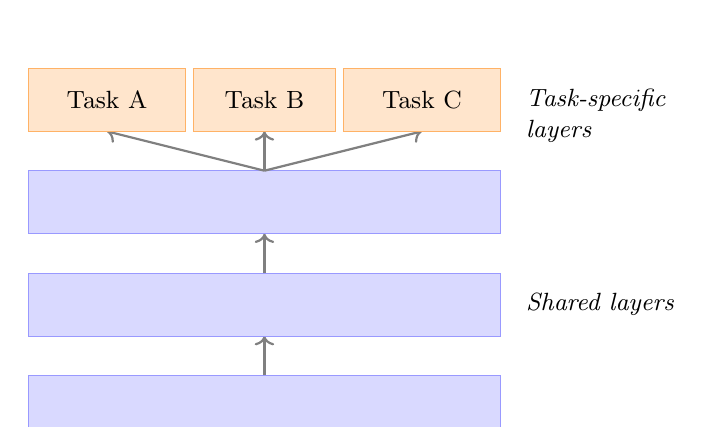
\begin{tikzpicture}[
    arr/.style={->, thick, gray}
]

    % Shared layer 1
    \fill[blue!15] (-3, 0) rectangle (3, 0.8);
    \draw[blue!40] (-3, 0) rectangle (3, 0.8);

    % Arrow between shared layer 1 and 2
    \draw[arr] (0, 0.8) -- (0, 1.3);

    % Shared layer 2
    \fill[blue!15] (-3, 1.3) rectangle (3, 2.1);
    \draw[blue!40] (-3, 1.3) rectangle (3, 2.1);

    % Arrow between shared layer 2 and 3
    \draw[arr] (0, 2.1) -- (0, 2.6);

    % Shared layer 3
    \fill[blue!15] (-3, 2.6) rectangle (3, 3.4);
    \draw[blue!40] (-3, 2.6) rectangle (3, 3.4);

    \node[right] at (3.2, 1.7) {\small \textit{Shared layers}};

    % Arrows from shared layer 3 to each task (diagonal)
    \draw[arr] (0, 3.4) -- (-2, 3.9);
    \draw[arr] (0, 3.4) -- (0,  3.9);
    \draw[arr] (0, 3.4) -- (2,  3.9);

    % Task-specific: 3 kotak terpisah
    \fill[orange!20] (-3,   3.9) rectangle (-1,   4.7);
    \fill[orange!20] (-0.9, 3.9) rectangle (0.9,  4.7);
    \fill[orange!20] (1,    3.9) rectangle (3,    4.7);
    \draw[orange!60] (-3,   3.9) rectangle (-1,   4.7);
    \draw[orange!60] (-0.9, 3.9) rectangle (0.9,  4.7);
    \draw[orange!60] (1,    3.9) rectangle (3,    4.7);

    \node at (-2,  4.3) {\small Task A};
    \node at (0,   4.3) {\small Task B};
    \node at (2,   4.3) {\small Task C};
    \node[right] at (3.2, 4.3) {\small \textit{Task-specific}};
    \node[right] at (3.2, 3.9) {\small \textit{layers}};

\end{tikzpicture}
\caption{Ilustrasi arsitektur \textit{hard parameter sharing} dalam
\textit{Multi-Task Learning} (\cite{ruder2017overview}, telah diolah
kembali)}
\label{fig:hard_sharing}
\end{figure}

Pada penelitian ini, pendekatan \textit{hard parameter sharing} diterapkan
dengan menjadikan \textit{autoencoder} sebagai jaringan bersama.
Representasi laten $\mathbf{z}$ yang dihasilkan oleh \textit{encoder}
digunakan secara bersamaan oleh dua \textit{head}: satu untuk pendeteksian
topik melalui \textit{clustering layer}, dan satu lagi untuk klasifikasi
sentimen melalui \textit{sentiment classifier}.

%-------------------------------------------------------------------------%
\subsection{\textit{Soft Parameter Sharing}}
%-------------------------------------------------------------------------%

\textit{Soft parameter sharing} mengambil pendekatan yang berbeda. Setiap
tugas memiliki model tersendiri dengan parameter masing-masing, namun
parameter antar model diatur agar tidak terlalu jauh berbeda melalui
regularisasi \parencite{ruder2017overview}. Salah satu cara yang umum
digunakan adalah menambahkan penalti $\ell_2$ terhadap perbedaan parameter
antar tugas:

\begin{equation}
    \mathcal{L}_{\text{soft}} = \sum_{t=1}^{T} \mathcal{L}_t(\theta_t)
    + \lambda \sum_{t=1}^{T} \sum_{t'=t+1}^{T}
    \|\theta_t - \theta_{t'}\|_2^2.
    \label{eq:soft_l2_reg}
\end{equation}

\noindent dengan $\lambda$ adalah skalar koefisien regularisasi yang mengontrol
seberapa mirip parameter antar tugas harus dijaga, dan
$\|\theta_t - \theta_{t'}\|_2^2$ mengukur seberapa jauh kedua set
parameter berbeda. Arsitektur \textit{soft parameter sharing}
diilustrasikan pada Gambar~\ref{fig:soft_sharing}.

\begin{figure}[H]
\centering
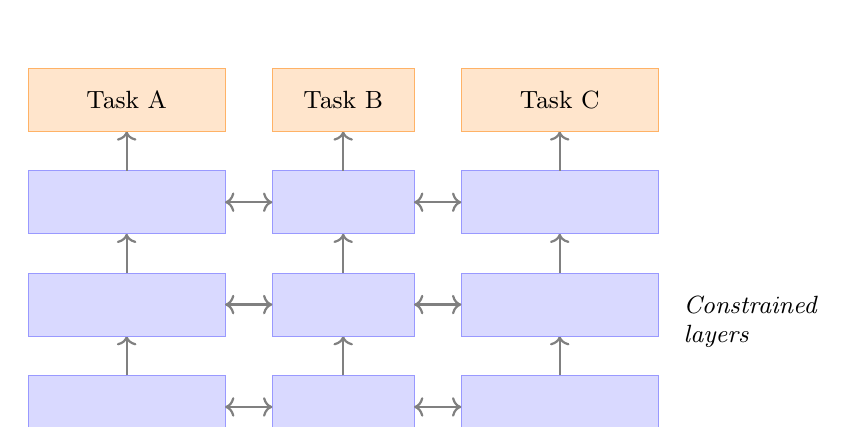
\begin{tikzpicture}[
    arr/.style={->, thick, gray},
    darr/.style={<->, thick, gray}
]
    % Constrained layer 1 (bottom)
    \fill[blue!15] (-4, 0) rectangle (-1.5, 0.8);
    \draw[blue!40] (-4, 0) rectangle (-1.5, 0.8);
    \fill[blue!15] (-0.9, 0) rectangle (0.9, 0.8);
    \draw[blue!40] (-0.9, 0) rectangle (0.9, 0.8);
    \fill[blue!15] (1.5, 0) rectangle (4, 0.8);
    \draw[blue!40] (1.5, 0) rectangle (4, 0.8);

    % Horizontal arrows layer 1
    \draw[darr] (-1.5, 0.4) -- (-0.9, 0.4);
    \draw[darr] (0.9, 0.4) -- (1.5, 0.4);

    % Arrows up layer 1 to 2
    \draw[arr] (-2.75, 0.8) -- (-2.75, 1.3);
    \draw[arr] (0, 0.8) -- (0, 1.3);
    \draw[arr] (2.75, 0.8) -- (2.75, 1.3);

    % Constrained layer 2 (middle)
    \fill[blue!15] (-4, 1.3) rectangle (-1.5, 2.1);
    \draw[blue!40] (-4, 1.3) rectangle (-1.5, 2.1);
    \fill[blue!15] (-0.9, 1.3) rectangle (0.9, 2.1);
    \draw[blue!40] (-0.9, 1.3) rectangle (0.9, 2.1);
    \fill[blue!15] (1.5, 1.3) rectangle (4, 2.1);
    \draw[blue!40] (1.5, 1.3) rectangle (4, 2.1);

    % Horizontal arrows layer 2
    \draw[darr] (-1.5, 1.7) -- (-0.9, 1.7);
    \draw[darr] (0.9, 1.7) -- (1.5, 1.7);

    % Arrows up layer 2 to 3
    \draw[arr] (-2.75, 2.1) -- (-2.75, 2.6);
    \draw[arr] (0, 2.1) -- (0, 2.6);
    \draw[arr] (2.75, 2.1) -- (2.75, 2.6);

    % Constrained layer 3 (top constrained)
    \fill[blue!15] (-4, 2.6) rectangle (-1.5, 3.4);
    \draw[blue!40] (-4, 2.6) rectangle (-1.5, 3.4);
    \fill[blue!15] (-0.9, 2.6) rectangle (0.9, 3.4);
    \draw[blue!40] (-0.9, 2.6) rectangle (0.9, 3.4);
    \fill[blue!15] (1.5, 2.6) rectangle (4, 3.4);
    \draw[blue!40] (1.5, 2.6) rectangle (4, 3.4);

    % Horizontal arrows layer 3
    \draw[darr] (-1.5, 3.0) -- (-0.9, 3.0);
    \draw[darr] (0.9, 3.0) -- (1.5, 3.0);

    \node[right] at (4.2, 1.7) {\small \textit{Constrained}};
    \node[right] at (4.2, 1.3) {\small \textit{layers}};

    % Arrows up to task boxes
    \draw[arr] (-2.75, 3.4) -- (-2.75, 3.9);
    \draw[arr] (0, 3.4) -- (0, 3.9);
    \draw[arr] (2.75, 3.4) -- (2.75, 3.9);

    % Task boxes
    \fill[orange!20] (-4, 3.9) rectangle (-1.5, 4.7);
    \draw[orange!60] (-4, 3.9) rectangle (-1.5, 4.7);
    \fill[orange!20] (-0.9, 3.9) rectangle (0.9, 4.7);
    \draw[orange!60] (-0.9, 3.9) rectangle (0.9, 4.7);
    \fill[orange!20] (1.5, 3.9) rectangle (4, 4.7);
    \draw[orange!60] (1.5, 3.9) rectangle (4, 4.7);

    \node at (-2.75, 4.3) {\small Task A};
    \node at (0, 4.3) {\small Task B};
    \node at (2.75, 4.3) {\small Task C};

\end{tikzpicture}
\caption{Ilustrasi arsitektur \textit{soft parameter sharing}
(\cite{ruder2017overview}, telah diolah kembali)}
\label{fig:soft_sharing}
\end{figure}

Perbedaan mendasar antara keduanya terletak pada bagaimana pengetahuan
dibagikan. Pada \textit{hard parameter sharing}, bobot benar-benar identik
sehingga semua tugas menggunakan representasi yang sama persis. Pada
\textit{soft parameter sharing}, setiap tugas tetap memiliki ruang belajar
sendiri namun didorong untuk tidak terlalu menyimpang, sehingga lebih
fleksibel namun membutuhkan lebih banyak parameter dan pengaturan
$\lambda$ yang tepat.

%-------------------------------------------------------------------------%
\section{\textit{Clustering}}
%-------------------------------------------------------------------------%

\textit{Clustering} merupakan teknik \textit{unsupervised learning} yang
mengelompokkan data berdasarkan kemiripan tanpa memerlukan label
\parencite{bezdek1984}. Berdasarkan cara pengelompokannya, terdapat dua
pendekatan utama. \textit{Hard clustering} membatasi setiap titik data ke
satu klaster, sedangkan \textit{soft clustering} memungkinkan satu titik
data masuk ke beberapa klaster sekaligus.

Metode \textit{clustering} dapat diklasifikasikan ke dalam beberapa
pendekatan, di antaranya \textit{centroid-based}, \textit{distribution-based},
\textit{connectivity-based}, dan \textit{density-based}. Penelitian ini
menggunakan pendekatan \textit{centroid-based clustering}, yaitu metode yang
memisahkan data berdasarkan jarak setiap titik data terhadap pusat klaster
(\textit{centroid}) \parencite{yusdiansyah2019}. Untuk mengukur jarak
tersebut digunakan jarak Euclidean:

\begin{equation}
    \|\mathbf{p} - \mathbf{q}\| =
    \sqrt{\sum_{d=1}^{D}(p_d - q_d)^2}.
    \label{eq:euclidean_distance}
\end{equation}

\noindent dengan $\mathbf{p} = (p_1, \ldots, p_D)$ dan
$\mathbf{q} = (q_1, \ldots, q_D)$ adalah dua vektor dalam ruang
berdimensi $D$.

Penelitian ini menggunakan \textit{Deep Embedded Clustering} (DEC)
\parencite{xie2016unsupervised} sebagai metode pendeteksian topik, yang
mempelajari representasi laten dan melakukan \textit{clustering} secara
bersamaan. DEC menerapkan \textit{soft clustering} melalui distribusi
probabilitas penugasan klaster, sehingga setiap ulasan dapat terhubung ke
lebih dari satu topik. Sebagai inisialisasi, DEC menggunakan K-Means untuk
menentukan pusat klaster awal di ruang \textit{embedding}.

%-------------------------------------------------------------------------%
\subsection{K-Means \textit{Clustering}}
%-------------------------------------------------------------------------%

K-Means merupakan algoritma \textit{centroid-based clustering} yang
mengelompokkan data dengan meminimalkan total jarak antara setiap titik
data dan pusat klasternya, dan termasuk ke dalam kategori \textit{hard
clustering} \parencite{macqueen1967some}.

Secara formal, misalkan terdapat himpunan data $X = \{\mathbf{x}_1,
\mathbf{x}_2, \ldots, \mathbf{x}_N\}$ dengan $\mathbf{x}_n \in
\mathbb{R}^D$ dan jumlah klaster yang diinginkan adalah $K$. K-Means
meminimalkan fungsi objektif berikut:

\begin{equation}
    J = \sum_{n=1}^{N} \sum_{k=1}^{K} r_{nk}
    \|\mathbf{x}_n - \boldsymbol{\mu}_k\|^2.
    \label{eq:kmeans_objective}
\end{equation}

\noindent dengan $\boldsymbol{\mu}_k$ adalah vektor \textit{centroid} klaster
ke-$k$, dan $r_{nk}$ adalah skalar variabel indikator biner yang bernilai
1 jika titik data $\mathbf{x}_n$ termasuk klaster ke-$k$ dan 0 jika
tidak. Nilai $J$ mengukur total kuadrat jarak seluruh titik data ke pusat
klasternya masing-masing.

Proses optimasi dilakukan secara iteratif melalui dua tahap yang
bergantian. Pada tahap pertama (\textit{assignment step}), setiap titik
data dialokasikan ke klaster dengan \textit{centroid} terdekat:

\begin{equation}
    r_{nk} = \begin{cases}
        1, & k = \arg\min_j \|\mathbf{x}_n - \boldsymbol{\mu}_j\|^2 \\
        0, & \text{yang lainnya.}
    \end{cases}
    \label{eq:assignment_step}
\end{equation}

\noindent dengan $\arg\min_j \|\mathbf{x}_n - \boldsymbol{\mu}_j\|^2$
menyatakan indeks $j$ yang meminimalkan nilai
$\|\mathbf{x}_n - \boldsymbol{\mu}_j\|^2$, yaitu indeks \textit{centroid}
terdekat terhadap titik data $\mathbf{x}_n$. Notasi $\arg\max$ yang
digunakan pada bagian-bagian selanjutnya memiliki pengertian yang serupa,
yaitu mengembalikan indeks yang memaksimalkan suatu fungsi.

Pada tahap kedua (\textit{update step}), \textit{centroid} setiap klaster
diperbarui menjadi rata-rata dari seluruh titik yang menjadi anggotanya:

\begin{equation}
    \boldsymbol{\mu}_k = \frac{\sum_{n=1}^{N} r_{nk}\,
    \mathbf{x}_n}{\sum_{n=1}^{N} r_{nk}}.
    \label{eq:centroid_update}
\end{equation}

Pembilang adalah jumlah posisi seluruh anggota klaster ke-$k$, sedangkan
penyebut adalah jumlah anggotanya. Dua tahap ini diulang sampai nilai $J$
tidak berubah signifikan atau jumlah iterasi mencapai batas maksimum.
Algoritma lengkapnya dapat dilihat pada Tabel~\ref{tab:kmeans_algorithm}.

\begin{table}[H]
\centering
\footnotesize
\setlength{\tabcolsep}{4pt}
\renewcommand{\arraystretch}{0.95}
\caption{Algoritma K-Means \textit{Clustering}}
\label{tab:kmeans_algorithm}
\resizebox{\textwidth}{!}{
\begin{tabular}{p{12cm}}
\toprule
\textbf{Algoritma K-Means \textit{Clustering}} \\
\midrule
\textbf{INPUT:} Himpunan data $\{\mathbf{x}_i\}_{i=1}^N$, banyak klaster
$K$, batas toleransi $\epsilon$, dan maksimal iterasi $\text{maxiter}$ \\
\midrule
1. Inisialisasi secara acak himpunan \textit{centroid}
   $\{\boldsymbol{\mu}_j\}_{j=1}^K$ \\
2. Tetapkan $\text{iter} = 0$ \\
3. \textbf{REPEAT} \\
4. \quad Tetapkan $\text{iter} = \text{iter} + 1$ \\
5. \quad \textit{Assignment step:} Cari nilai
$r_{nk} =
\begin{cases}
1, & k = \arg\min_j \|\mathbf{x}_n - \boldsymbol{\mu}_j\|^2 \\
0, & \text{yang lainnya}
\end{cases}$ \\
6. \quad \textit{Update step:} Cari nilai
$\boldsymbol{\mu}_k =
\frac{\sum_{n=1}^N r_{nk} \mathbf{x}_n}{\sum_{n=1}^N r_{nk}}$ \\
7. \quad Hitung
$J = \sum_{n=1}^N \sum_{k=1}^K r_{nk}
\|\mathbf{x}_n - \boldsymbol{\mu}_k\|^2$ \\
8. \textbf{UNTIL} $J < \epsilon$ \textbf{OR}
   $\text{iter} > \text{maxiter}$ \\
9. Untuk setiap $n = 1, 2, \ldots, N$, tetapkan nilai
   $u_n = \arg\max_k (r_{nk})$, dengan $k = 1, 2, \ldots, K$ \\
10. Bentuk $\{C_1, C_2, \ldots, C_K\}$, dengan $C_k$ merupakan himpunan
    anggota data $\mathbf{x}_i$ di mana $u_i = k$ \\
11. \textbf{STOP} \\
\midrule
\textbf{OUTPUT:} Nilai keanggotaan $\{u_n\}_{n=1}^N$ dan himpunan klaster
$\{C_k\}_{k=1}^K$ \\
\bottomrule
\end{tabular}
}
\end{table}

%-------------------------------------------------------------------------%
\section{Interpretabilitas Model \textit{Deep Learning}}
%-------------------------------------------------------------------------%

Interpretabilitas model \textit{deep learning} merujuk pada kemampuan
untuk memahami dan menjelaskan keputusan yang dihasilkan oleh model yang
bersifat \textit{black-box} \parencite{sundararajan2017axiomatic}. Dalam
konteks pemrosesan bahasa alami, interpretabilitas penting karena model
perlu mampu menjelaskan mengapa suatu teks diklasifikasikan ke dalam
kategori tertentu, terutama pada aplikasi analisis sentimen dan
pengelompokan topik.

Secara umum, metode interpretabilitas dapat dikategorikan menjadi dua
kelompok \parencite{li2016visualizing}. Kelompok pertama adalah metode
\textit{intrinsic}, yaitu model yang secara bawaan dapat diinterpretasi
seperti pohon keputusan dan regresi linier. Kelompok kedua adalah metode
\textit{post-hoc}, yaitu metode yang diterapkan setelah model dilatih
untuk menganalisis perilaku model yang kompleks tanpa mengubah
arsitekturnya.

Dalam penelitian ini, metode \textit{post-hoc} digunakan untuk menganalisis
kontribusi setiap token terhadap prediksi sentimen model, yaitu
\textit{occlusion-based token attribution} dan \textit{Integrated
Gradients}.

%-------------------------------------------------------------------------%
\subsection{\textit{Occlusion-based Token Attribution}}
%-------------------------------------------------------------------------%

\textit{Occlusion-based token attribution} merupakan salah satu metode
\textit{post-hoc} yang banyak digunakan untuk menginterpretasi model
berbasis teks \parencite{zeiler2014visualizing, li2016visualizing}. Metode
ini mengukur pentingnya suatu token dengan cara menggantinya dan mengamati
perubahan prediksi model.

Pada model berbasis \textit{transformer} seperti BERT, oklusi dilakukan
dengan mengganti token target menggunakan token khusus \texttt{[MASK]},
sehingga model tetap menerima input dengan panjang yang sama. Pendekatan
ini dikenal sebagai \textit{leave-one-out attribution}.

Secara formal, diberikan teks input $\mathbf{x} = (x_1, x_2, \ldots,
x_T)$ yang terdiri dari $T$ token, representasi kontekstual diperoleh
melalui BERT sebagai:

\begin{equation}
    \mathbf{h} = \text{BERT}(\mathbf{x}) \in \mathbb{R}^d.
    \label{eq:bert_cls}
\end{equation}

\noindent dengan $\mathbf{h}$ merupakan vektor representasi \texttt{[CLS]} dari
lapisan terakhir BERT. Representasi ini kemudian diteruskan ke lapisan
klasifikasi sentimen untuk menghasilkan distribusi probabilitas:

\begin{equation}
    f(\mathbf{x}) = \text{softmax}(\mathbf{W} \cdot \mathbf{h} + \mathbf{b})
    \in \mathbb{R}^C.
    \label{eq:sentiment_pred}
\end{equation}

\noindent dengan $C$ adalah jumlah kelas sentimen, $\mathbf{W}$ adalah matriks
bobot dan $\mathbf{b}$ adalah vektor bias lapisan klasifikasi. Skor
atribusi token $x_i$ terhadap kelas sentimen $c$ didefinisikan sebagai
selisih probabilitas prediksi sebelum dan sesudah oklusi:

\begin{equation}
    \text{Attr}(x_i, c) = f_c(\mathbf{x}) -
    f_c(\mathbf{x}_{\setminus i}).
    \label{eq:occlusion}
\end{equation}

\noindent dengan $f_c(\mathbf{x})$ adalah skalar probabilitas prediksi kelas $c$
pada teks asli, dan $f_c(\mathbf{x}_{\setminus i})$ adalah skalar
probabilitas prediksi setelah token $x_i$ diganti dengan \texttt{[MASK]}.
Nilai positif berarti token $x_i$ mendukung prediksi kelas $c$, nilai
negatif berarti token menekannya, dan nilai mendekati nol berarti token
tidak berpengaruh signifikan.

Dibandingkan dengan metode berbasis gradien, \textit{occlusion-based
attribution} lebih mudah diinterpretasi karena tidak bergantung pada
komputasi turunan yang kompleks. Namun, metode ini memiliki kompleksitas
waktu $\mathcal{O}(T)$ terhadap panjang token sehingga lebih mahal secara
komputasi untuk teks yang panjang \parencite{li2016visualizing}.

%-------------------------------------------------------------------------%
\subsection{\textit{Integrated Gradients}}
%-------------------------------------------------------------------------%

\textit{Integrated Gradients} (IG) merupakan metode atribusi berbasis
gradien yang diusulkan oleh \parencite{sundararajan2017axiomatic}. Berbeda
dengan \textit{occlusion-based attribution} yang bersifat diskrit, IG
menghitung kontribusi setiap dimensi input secara kontinu dengan
mengintegrasikan gradien prediksi model sepanjang jalur lurus dari
\textit{baseline} menuju input asli.

Secara formal, diberikan vektor input $\mathbf{x} \in \mathbb{R}^d$ dan
vektor \textit{baseline} $\mathbf{x'} \in \mathbb{R}^d$ yang umumnya
berupa vektor nol, atribusi IG untuk dimensi ke-$i$ didefinisikan sebagai:

\begin{equation}
    \text{IG}_i(\mathbf{x}) = (x_i - x'_i) \times
    \int_{\alpha=0}^{1}
    \frac{\partial f\big(\mathbf{x'} + \alpha(\mathbf{x} -
    \mathbf{x'})\big)}{\partial x_i} \, d\alpha.
    \label{eq:ig}
\end{equation}

\noindent dengan $\alpha$ adalah skalar parameter yang menunjukkan posisi pada
jalur dari \textit{baseline} menuju input asli, dan
$\frac{\partial f}{\partial x_i}$ adalah skalar gradien prediksi terhadap
dimensi ke-$i$. Dalam praktiknya, integral tersebut diaproksimasi
menggunakan \textit{Riemann sum} dengan $m$ langkah interpolasi:

\begin{equation}
    \text{IG}_i(\mathbf{x}) \approx (x_i - x'_i) \times
    \sum_{k=1}^{m}
    \frac{\partial f\Big(\mathbf{x'} + \frac{k}{m}
    (\mathbf{x} - \mathbf{x'})\Big)}{\partial x_i} \times
    \frac{1}{m}.
    \label{eq:ig_approx}
\end{equation}

Metode IG memenuhi dua karakteristik penting, yaitu \textit{sensitivity}
dan \textit{implementation invariance}
\parencite{sundararajan2017axiomatic}. \textit{Sensitivity} menjamin bahwa
apabila suatu fitur mempengaruhi prediksi model, fitur tersebut akan
mendapatkan atribusi bernilai tidak nol. \textit{Implementation invariance}
menjamin bahwa dua model yang secara fungsional ekuivalen akan menghasilkan
atribusi yang sama meskipun memiliki implementasi internal yang berbeda.
%-----------------------------------------------------------------------------%
\chapter{\babTiga}
%-----------------------------------------------------------------------------%

Bab ini menjelaskan rancangan dan implementasi metode yang diusulkan, mulai dari penggunaan BERT sebagai \textit{feature extractor}, arsitektur model \textit{joint sentiment-topic} berbasis \textit{multitask learning}, peran \textit{autoencoder} dalam kompresi representasi, pengelompokan topik dengan \textit{Deep Embedded Clustering} (DEC), interpretasi model melalui analisis atribusi token, hingga evaluasi kualitas topik.

\begin{figure}[H]
    \centering
    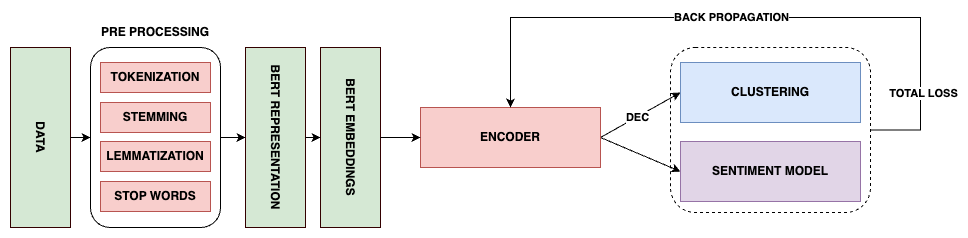
\includegraphics[width=0.9\textwidth]{assets/pics/MTL/FNN1.png}
    \caption{Alur metode analisis sentimen dan pendeteksian topik}
    \label{fig:alur_metode}
\end{figure}

%-----------------------------------------------------------------------------%
\section{\textit{Bidirectional Encoder Representations from Transformers}
(BERT) Sebagai Model Representasi Teks}
\label{sec:bert}
%-----------------------------------------------------------------------------%

Terdapat dua pendekatan utama dalam pemanfaatan model BERT, yaitu \textit{feature-based} dan \textit{fine-tuning}. Pada pendekatan \textit{feature-based}, BERT berfungsi sebagai \textit{feature extractor} tanpa mengubah parameter internalnya. Pada pendekatan \textit{fine-tuning}, lapisan keluaran khusus ditambahkan dan seluruh bobot dilatih ulang secara \textit{end-to-end}.

Pada penelitian ini, BERT digunakan melalui pendekatan \textit{feature-based} dengan bobot yang dibekukan sepenuhnya (\textit{frozen}). Representasi yang dihasilkan kemudian digunakan sebagai \textit{input} untuk \textit{autoencoder} dan pengelompokan topik menggunakan DEC. Contoh representasi teks yang dihasilkan BERT ditunjukkan pada Gambar~\ref{fig:bert_representasi}.

\begin{figure}[H]
    \centering
    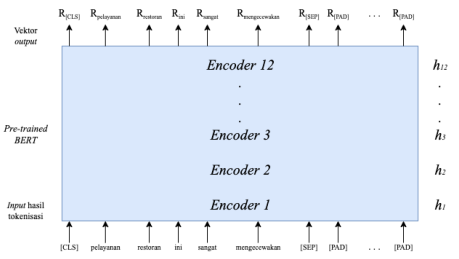
\includegraphics[width=0.7\textwidth]{assets/pics/BERT/BERT Rep-2.png}
    \caption{Representasi teks menggunakan BERT
             (\parencite{devlin2018bert}; telah diolah kembali).}
    \label{fig:bert_representasi}
\end{figure}

Sebagai ilustrasi, misalkan kalimat \textit{input} yang digunakan adalah \textit{``pelayanan restoran ini sangat mengecewakan''}. Proses pembentukan representasi teks oleh BERT dilakukan melalui beberapa tahapan berikut.

\begin{enumerate}
    \item \textbf{Tokenisasi.} Kalimat dipecah menjadi token menggunakan \textit{WordPiece tokenizer}, lalu ditambahkan token khusus \texttt{[CLS]} di awal dan \texttt{[SEP]} di akhir:
    \begin{center}
        \texttt{[[CLS], pelayanan, restoran, ini, sangat, mengecewakan, [SEP]]}.
    \end{center}

    \item \textbf{\textit{Padding}.} Token \texttt{[PAD]} ditambahkan agar panjang seluruh urutan seragam, misalnya hingga 10 token:
    \begin{center}
        \texttt{[[CLS], pelayanan, restoran, ini, sangat, mengecewakan, [SEP],
        [PAD], [PAD], [PAD]]}.
    \end{center}

    \item \textbf{\textit{Attention Mask}.} Dibuat \textit{attention mask} untuk membedakan token bermakna dengan token \textit{padding}. Token selain \texttt{[PAD]} diberi nilai 1 dan \texttt{[PAD]} diberi nilai 0:
    \begin{center}
        \textit{attention mask} $= [1, 1, 1, 1, 1, 1, 1, 0, 0, 0]$.
    \end{center}

    \item \textbf{\textit{Embedding}.} Token diubah menjadi representasi numerik melalui lapisan \textit{embedding}, yaitu hasil penjumlahan dari \textit{token embedding}, \textit{segment embedding}, dan \textit{position embedding}.

    \item \textbf{\textit{Encoding}.} Representasi diproses melalui beberapa lapisan \textit{encoder}, di mana setiap lapisan terdiri atas mekanisme \textit{multi-head self-attention}, \textit{feed-forward network}, koneksi residu, dan normalisasi.
\end{enumerate}

Model BERT \textit{pre-trained} yang digunakan terdiri atas 12 lapisan \textit{encoder} dengan ukuran \textit{hidden size} sebesar 768. Misalkan $t$ adalah panjang maksimum token dan $M$ adalah jumlah teks dalam \textit{dataset}, maka keluaran BERT berupa matriks berukuran $M \times t \times 768$. Pada penelitian ini, $t = 128$.

Pada tahap \textit{clustering}, representasi setiap teks harus berupa vektor, bukan matriks. Oleh karena itu, digunakan strategi ekstraksi token \texttt{[CLS]}, yang diletakkan di awal setiap urutan dan dilatih untuk merepresentasikan konteks global kalimat. Misalkan $\mathbf{H} = (h_{ij}) \in \mathbb{R}^{t \times 768}$ adalah matriks keluaran BERT untuk suatu teks, dengan $\mathbf{h}_i = (h_{i1}, h_{i2}, \ldots, h_{i,768})$ menyatakan representasi token ke-$i$. Vektor representasi dokumen $\mathbf{f}$ diperoleh dari baris pertama $\mathbf{H}$:

\begin{equation}
    \mathbf{f} = \mathbf{h}_1 \in \mathbb{R}^{768}
    \label{eq:cls_extraction}
\end{equation}

Vektor $\mathbf{f}$ ini selanjutnya digunakan sebagai \textit{input} untuk \textit{autoencoder} pada tahap berikutnya.

%-----------------------------------------------------------------------------%
\section{Model \textit{Joint Sentiment-Topic} Berbasis \textit{Multitask
Learning}}
%-----------------------------------------------------------------------------%

Penelitian ini mengusulkan model \textit{Joint Sentiment-Topic} berbasis \textit{Multitask Learning} untuk melakukan analisis sentimen dan pendeteksian topik secara bersamaan. Model ini dibangun di atas representasi BERT yang diproses melalui \textit{autoencoder} untuk menghasilkan representasi laten berdimensi rendah. Representasi laten tersebut digunakan bersama oleh dua \textit{head}, yaitu \textit{sentiment head} untuk klasifikasi sentimen dan \textit{clustering head} untuk pendeteksian topik melalui DEC. Pendekatan ini mengikuti skema \textit{hard parameter sharing}, di mana lapisan \textit{encoder} pada \textit{autoencoder} berfungsi sebagai jaringan bersama yang menerima gradien dari kedua tugas secara simultan.

Alur model terdiri atas tiga tahap. Pertama, representasi BERT berdimensi 768 diperoleh dari tahap ekstraksi fitur pada Bagian~\ref{sec:bert}. Kedua, representasi tersebut dikompresi oleh \textit{encoder} menjadi vektor laten $\mathbf{z}$ berdimensi lebih rendah. Ketiga, $\mathbf{z}$ digunakan secara bersamaan oleh kedua \textit{head} dalam satu kerangka optimasi bersama. Total \textit{loss} yang dioptimalkan selama pelatihan \textit{multitask} didefinisikan sebagai:

\begin{equation}
    \mathcal{L}_{\text{total}} = \gamma \cdot \mathcal{L}_{\text{KLD}}
    + \eta \cdot \mathcal{L}_{\text{CE}}
    \label{eq:total_loss}
\end{equation}

\noindent dengan $\gamma$ dan $\eta$ adalah koefisien bobot yang mengontrol kontribusi relatif antara \textit{loss} \textit{clustering} dan \textit{loss} klasifikasi sentimen.

%-----------------------------------------------------------------------------%
\section{Implementasi \textit{Autoencoder}}
%-----------------------------------------------------------------------------%

\textit{Autoencoder} umumnya sulit dilatih langsung karena rentan \textit{overfitting} dan sulit menemukan representasi yang stabil. Oleh karena itu, sebelum pelatihan \textit{multitask}, \textit{autoencoder} terlebih dahulu dilatih secara \textit{unsupervised} melalui proses \textit{pretraining} sebagai inisialisasi bobot awal.

Gambar~\ref{fig:autoencoder} menunjukkan ilustrasi arsitektur yang digunakan, mulai dari \textit{autoencoder} lengkap hingga komponen \textit{encoder} yang dipertahankan setelah \textit{pretraining}.

\begin{figure}[H]
    \centering
    \begin{subfigure}[b]{0.45\textwidth}
        \centering
        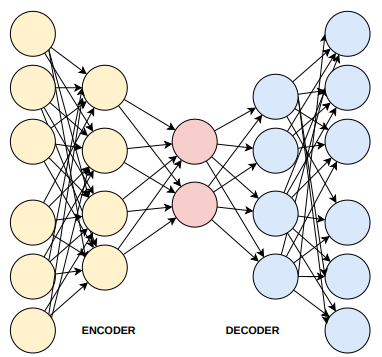
\includegraphics[height=5cm]{assets/pics/Autoencoder/Autoencoder0.png}
        \caption{\textit{Autoencoder} lengkap}
        \label{fig:autoencoder-full}
    \end{subfigure}
    \hfill
    \begin{subfigure}[b]{0.45\textwidth}
        \centering
        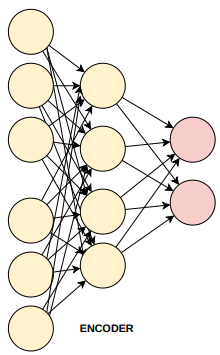
\includegraphics[height=5cm]{assets/pics/Autoencoder/Autoencoder1.png}
        \caption{\textit{Encoder}}
        \label{fig:encoder}
    \end{subfigure}
    \caption{Ilustrasi \textit{autoencoder} lengkap (kiri) dan komponen
    \textit{encoder} setelah \textit{decoder} dilepas (kanan).}
    \label{fig:autoencoder}
\end{figure}

Pada tahap \textit{pretraining}, jaringan dilatih untuk merekonstruksi kembali data \textit{input} dari representasi laten yang dihasilkan \textit{encoder}. Fungsi \textit{loss} yang digunakan adalah \textit{Mean Squared Error} (MSE) antara vektor \textit{input} asli dan hasil rekonstruksinya:

\begin{equation}
    \mathcal{L}_{\text{MSE}} = \frac{1}{N} \sum_{i=1}^{N}
    \left\| \mathbf{f}_i - \hat{\mathbf{f}}_i \right\|^2
    \label{eq:mse}
\end{equation}

\noindent dengan $N$ adalah jumlah total sampel, $\mathbf{f}_i$ adalah vektor representasi BERT ke-$i$, dan $\hat{\mathbf{f}}_i$ adalah hasil rekonstruksinya.

Fungsi aktivasi yang digunakan pada lapisan \textit{encoder} dan \textit{decoder} adalah \textit{Rectified Linear Unit} (ReLU), yang dipilih karena sesuai dengan distribusi representasi BERT yang dominan bernilai positif. 

Setelah \textit{pretraining} selesai, bobot \textit{encoder} digunakan sebagai inisialisasi untuk pelatihan \textit{multitask}. Pada tahap ini \textit{encoder} dipertahankan dan dioptimalkan bersama kedua \textit{head}, sedangkan \textit{decoder} tidak lagi digunakan. Representasi laten $\mathbf{z} = f_\theta(\mathbf{f})$ yang dihasilkan \textit{encoder} digunakan bersama oleh \textit{sentiment head} dan \textit{clustering head}.

%-----------------------------------------------------------------------------%
\section{Analisis Sentimen Menggunakan \textit{Sentiment Head}}
%-----------------------------------------------------------------------------%

Vektor laten $\mathbf{z} \in \mathbb{R}^{256}$ yang dihasilkan \textit{encoder} diteruskan ke \textit{sentiment head} untuk diklasifikasikan ke salah satu dari dua kelas sentimen. Arsitektur \textit{sentiment head} terdiri atas tiga lapisan linear bertingkat dengan dimensi $256 \to 256 \to 32 \to 2$. Setiap lapisan tersembunyi dilengkapi dengan \textit{batch normalization}, fungsi aktivasi \textit{Gaussian Error Linear Unit} (GELU), dan \textit{dropout} dengan probabilitas $p = 0{,}5$. Lapisan keluaran berdimensi dua diikuti fungsi \textit{softmax} untuk menghasilkan distribusi probabilitas antarkelas. Arsitektur lengkapnya diilustrasikan pada Gambar~\ref{fig:sentiment_head} berikut.

\begin{figure}[H]
\centering
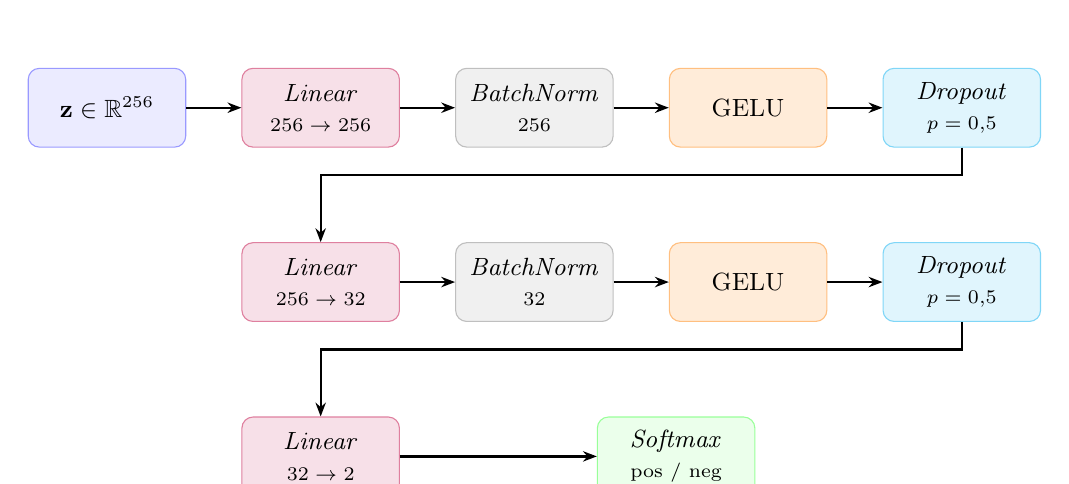
\begin{tikzpicture}[
    node distance=0.4cm and 0.7cm,
    box/.style={rectangle, rounded corners=4pt, draw, align=center,
                font=\small, minimum height=1cm, minimum width=2cm},
    inbox/.style={box,  fill=blue!8,    draw=blue!40},
    fcbox/.style={box,  fill=purple!12, draw=purple!50},
    bnbox/.style={box,  fill=gray!12,   draw=gray!50},
    actbox/.style={box, fill=orange!15, draw=orange!50},
    dropbox/.style={box,fill=cyan!12,   draw=cyan!50},
    outbox/.style={box, fill=green!8,   draw=green!40},
    arrow/.style={-{Stealth[length=5pt]}, thick}
]

\node[inbox] (z) {$\mathbf{z} \in \mathbb{R}^{256}$};

\node[fcbox,   right=of z]    (fc1)   {\textit{Linear}\\{\scriptsize$256 \to 256$}};
\node[bnbox,   right=of fc1]  (bn1)   {\textit{BatchNorm}\\{\scriptsize$256$}};
\node[actbox,  right=of bn1]  (gelu1) {GELU};
\node[dropbox, right=of gelu1](drop1) {\textit{Dropout}\\{\scriptsize$p=0{,}5$}};

\node[fcbox,   below=1.2cm of fc1]   (fc2)   {\textit{Linear}\\{\scriptsize$256 \to 32$}};
\node[bnbox,   right=of fc2]         (bn2)   {\textit{BatchNorm}\\{\scriptsize$32$}};
\node[actbox,  right=of bn2]         (gelu2) {GELU};
\node[dropbox, right=of gelu2]       (drop2) {\textit{Dropout}\\{\scriptsize$p=0{,}5$}};

\node[fcbox,  below=1.2cm of fc2]    (fc3)     {\textit{Linear}\\{\scriptsize$32 \to 2$}};
\node[outbox, right=2.5cm of fc3]    (softmax) {\textit{Softmax}\\{\scriptsize pos / neg}};

\draw[arrow] (z)     -- (fc1);
\draw[arrow] (fc1)   -- (bn1);
\draw[arrow] (bn1)   -- (gelu1);
\draw[arrow] (gelu1) -- (drop1);
\draw[arrow] (drop1.south) -- ++(0,-0.35) -| (fc2.north);
\draw[arrow] (fc2)   -- (bn2);
\draw[arrow] (bn2)   -- (gelu2);
\draw[arrow] (gelu2) -- (drop2);
\draw[arrow] (drop2.south) -- ++(0,-0.35) -| (fc3.north);
\draw[arrow] (fc3)   -- (softmax);

\end{tikzpicture}
\caption{Arsitektur \textit{sentiment head}.}
\label{fig:sentiment_head}
\end{figure}

Proses klasifikasi dirumuskan sebagai:

\begin{equation}
    \hat{\mathbf{y}} = \text{softmax}\!\left(\mathbf{W}_c \mathbf{z}
    + \mathbf{b}_c\right)
    \label{eq:sentiment_cls}
\end{equation}

\noindent dengan $\mathbf{W}_c$ dan $\mathbf{b}_c$ masing-masing adalah bobot dan bias pada lapisan keluaran. Fungsi \textit{softmax} mengubah nilai logit menjadi distribusi probabilitas, di mana setiap elemen $\hat{y}_i \in [0, 1]$ dan $\sum_i \hat{y}_i = 1$.

Selama pelatihan, prediksi $\hat{\mathbf{y}}$ dibandingkan dengan label sebenarnya $\mathbf{y}$ menggunakan fungsi \textit{loss Categorical Cross-Entropy}:

\begin{equation}
    \mathcal{L}_{\text{CE}} = -\sum_{i=1}^{N} \sum_{j=1}^{2}
    y_{ij} \log \hat{y}_{ij}
    \label{eq:ce_loss}
\end{equation}

\noindent dengan $N$ adalah jumlah sampel, $y_{ij}$ adalah label aktual dalam bentuk \textit{one-hot} bernilai 1 jika sampel ke-$i$ termasuk kelas ke-$j$ dan 0 jika tidak, serta $\hat{y}_{ij}$ adalah probabilitas prediksi model. $\mathcal{L}_{\text{CE}}$ ini menjadi salah satu komponen dari total \textit{loss} pada Persamaan~\eqref{eq:total_loss}.

%-----------------------------------------------------------------------------%
\section{\textit{Deep Embedded Clustering} (DEC) dan \textit{Clustering Head}}
%-----------------------------------------------------------------------------%

Selain \textit{sentiment head}, vektor laten $\mathbf{z}$ yang sama diteruskan ke \textit{clustering head} untuk pendeteksian topik. \textit{Clustering head} diimplementasikan menggunakan DEC, yang bertujuan memperbarui representasi laten dan menyesuaikan posisi \textit{centroid} agar sesuai dengan struktur distribusi data pada ruang laten \parencite{xie2016unsupervised}. Berbeda dengan \textit{hard assignment} yang menetapkan setiap sampel ke satu klaster, DEC menggunakan distribusi probabilistik sehingga setiap sampel memiliki derajat keanggotaan terhadap seluruh klaster. Arsitektur \textit{clustering head} diilustrasikan pada Gambar~\ref{fig:clustering_head} berikut.

\begin{figure}[H]
\centering
\resizebox{\textwidth}{!}{%
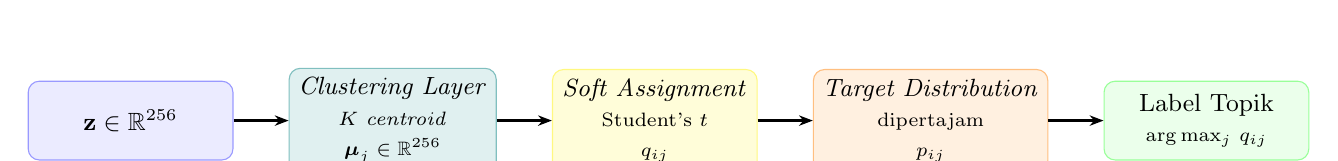
\begin{tikzpicture}[
    node distance=0.4cm and 0.7cm,
    box/.style={rectangle, rounded corners=4pt, draw, align=center,
                font=\small, minimum height=1cm, minimum width=2.6cm},
    inbox/.style={box,  fill=blue!8,    draw=blue!40},
    cbox/.style={box,   fill=teal!12,   draw=teal!50},
    distbox/.style={box,fill=yellow!15, draw=yellow!50},
    targbox/.style={box,fill=orange!12, draw=orange!50},
    outbox/.style={box, fill=green!8,   draw=green!40},
    arrow/.style={-{Stealth[length=5pt]}, thick}
]

\node[inbox] (z) {$\mathbf{z} \in \mathbb{R}^{256}$};

\node[cbox,    right=of z]    (cent)
    {\textit{Clustering Layer}\\
     {\scriptsize$K$ \textit{centroid}}\\
     {\scriptsize$\boldsymbol{\mu}_j \in \mathbb{R}^{256}$}};

\node[distbox, right=of cent] (soft)
    {\textit{Soft Assignment}\\
     {\scriptsize Student's $t$}\\
     {\scriptsize$q_{ij}$}};

\node[targbox, right=of soft] (target)
    {\textit{Target Distribution}\\
     {\scriptsize dipertajam}\\
     {\scriptsize$p_{ij}$}};

\node[outbox,  right=of target] (label)
    {Label Topik\\
     {\scriptsize$\arg\max_j\, q_{ij}$}};

\draw[arrow] (z)      -- (cent);
\draw[arrow] (cent)   -- (soft);
\draw[arrow] (soft)   -- (target);
\draw[arrow] (target) -- (label);

\end{tikzpicture}%
}
\caption{Arsitektur \textit{clustering head} berbasis DEC.}
\label{fig:clustering_head}
\end{figure}

Proses DEC dimulai dengan inisialisasi \textit{centroid} menggunakan K-Means pada representasi laten awal hasil \textit{pretraining autoencoder}. Selanjutnya, distribusi \textit{soft assignment} $q_{ij}$ untuk setiap data $\mathbf{z}_i$ terhadap \textit{centroid} $\boldsymbol{\mu}_j$ dihitung menggunakan distribusi Student's $t$:

\begin{equation}
    q_{ij} = \frac{\left(1 + \left\|\mathbf{z}_i -
    \boldsymbol{\mu}_j\right\|^2\right)^{-1}}
    {\displaystyle\sum_{j'=1}^{K}\left(1 + \left\|\mathbf{z}_i -
    \boldsymbol{\mu}_{j'}\right\|^2\right)^{-1}}
    \label{eq:soft_assign}
\end{equation}

\noindent dengan $q_{ij}$ menyatakan probabilitas sampel $i$ termasuk klaster $j$, dan $K$ adalah jumlah klaster.

Selanjutnya, DEC mendefinisikan distribusi target $p_{ij}$ yang lebih 
terkonsentrasi (\textit{sharpened}) agar setiap sampel lebih condong ke 
satu klaster. Misalkan $f_j = \sum_{i} q_{ij}$ adalah frekuensi 
\textit{soft} klaster $j$, maka:

\begin{equation}
    p_{ij} = \frac{q_{ij}^2 \,/\, f_j}
    {\displaystyle\sum_{j'=1}^{K} q_{ij'}^2 \,/\, f_{j'}}
    \label{eq:target_dist}
\end{equation}

Pembagian dengan $f_j$ mencegah klaster besar mendominasi proses 
optimasi, sedangkan kuadrat pada $q_{ij}$ membuat distribusi lebih 
terkonsentrasi pada satu klaster. Optimasi dilakukan dengan meminimalkan 
\textit{Kullback-Leibler Divergence} antara distribusi target $P$ dan 
distribusi \textit{soft assignment} $Q$:

\begin{equation}
    \mathcal{L}_{\text{KLD}} = \sum_{i}\sum_{j}
    p_{ij} \log\frac{p_{ij}}{q_{ij}}
    \label{eq:kld}
\end{equation}

\noindent $\mathcal{L}_{\text{KLD}}$ digunakan sebagai dasar untuk memperbarui parameter \textit{encoder} dan posisi \textit{centroid} menggunakan optimizer Adam secara iteratif. Pada setiap \textit{update interval}, label klaster hasil iterasi sebelumnya akan dibandingkan dengan label terbaru. Proses pelatihan dihentikan apabila perubahan label klaster ($\Delta_{\text{label}}$) berada di bawah batas toleransi $\tau$. Prosedur lengkap metode ini disajikan pada Tabel~\ref{tab:alg_dec} berikut.

\begin{table}[H]
\centering
\caption{Algoritma \textit{Deep Embedded Clustering} (DEC)}
\label{tab:alg_dec}
\begin{tabular}{p{0.05\textwidth} p{0.85\textwidth}}
\hline
\multicolumn{2}{l}{\textbf{Algoritma} \textit{Deep Embedded Clustering} (DEC)} \\
\hline
\multicolumn{2}{l}{\textbf{INPUT} \hspace{1.2em}
    Himpunan vektor data $\{\mathbf{f}_i\}_{i=1}^{N} \in \mathbb{R}^{768}$;
    jumlah klaster $K$;} \\
\multicolumn{2}{l}{\hspace{4.7em}
    \textit{batch size} $b$; batas toleransi konvergensi $\tau$;} \\
\multicolumn{2}{l}{\hspace{4.7em}
    parameter bobot \textit{loss} $\gamma$, $\eta$;
    jumlah iterasi maksimum $T_{\max}$} \\[2pt]
\multicolumn{2}{l}{\textbf{OUTPUT}
    Representasi laten $\{\mathbf{z}_i\}$;
    label klaster $\{y_{\text{cluster}}\}$;
    label sentimen $\{y_{\text{sentiment}}\}$} \\
\hline
1. & Latih \textit{autoencoder} dengan meminimalkan MSE: \\
   & \hspace{1.5em}
     $\mathcal{L}_{\text{MSE}} = \dfrac{1}{N}\displaystyle\sum_{i=1}^{N}
     \|\mathbf{f}_i - \hat{\mathbf{f}}_i\|^2$ \\[6pt]
2. & Ambil bagian \textit{encoder} untuk memperoleh representasi laten
     $\mathbf{z}_i = f_\theta(\mathbf{f}_i)$ \\[3pt]
3. & Inisialisasi \textit{centroid} awal $\{\boldsymbol{\mu}_j\}_{j=1}^{K}$
     menggunakan K-Means pada $\{\mathbf{z}_i\}$ \\[3pt]
4. & \textbf{FOR} iter $= 1$ hingga $T_{\max}$ \\[3pt]
   & \hspace{1em} 4.1 \hspace{0.5em}
     Simpan label klaster sebelumnya $y_{\text{prev}}$ \\[3pt]
   & \hspace{1em} 4.2 \hspace{0.5em}
     Proyeksikan data ke ruang laten: $\mathbf{z}_i = f_\theta(\mathbf{f}_i)$ \\[3pt]
   & \hspace{1em} 4.3 \hspace{0.5em}
     Hitung \textit{soft assignment} $q_{ij}$ menggunakan distribusi
     Student's $t$ \\[3pt]
   & \hspace{1em} 4.4 \hspace{0.5em}
     Hitung distribusi target $p_{ij}$ berdasarkan $q_{ij}$ \\[3pt]
   & \hspace{1em} 4.5 \hspace{0.5em}
     Hitung keluaran sentimen
     $\hat{\mathbf{y}} = \text{softmax}(\mathbf{W}_c\mathbf{z} +
     \mathbf{b}_c)$ \\[3pt]
   & \hspace{1em} 4.6 \hspace{0.5em}
     Perbarui parameter model dengan meminimalkan \textit{joint loss}: \\
   & \hspace{3em}
     $\mathcal{L}_{\text{total}} = \gamma \cdot \mathcal{L}_{\text{KLD}}(P,
     Q) + \eta \cdot \mathcal{L}_{\text{CE}}(\mathbf{y}, \hat{\mathbf{y}})$ \\[3pt]
   & \hspace{1em} 4.7 \hspace{0.5em}
     Jika $\Delta_{\text{label}} < \tau$, hentikan pelatihan \\[3pt]
5. & \textbf{END FOR} \\[3pt]
6. & Simpan bobot terbaik model berdasarkan metrik validasi \\
\hline
\multicolumn{2}{l}{\textbf{OUTPUT:}
    Representasi laten $\{\mathbf{z}_i\}$,
    label klaster $\{y_{\text{cluster}}\}$,
    dan label sentimen $\{y_{\text{sentiment}}\}$} \\
\hline
\end{tabular}
\end{table}

%-----------------------------------------------------------------------------%
\section{Pelatihan \textit{Joint} dengan \textit{Multitask Loss}}
%-----------------------------------------------------------------------------%

Total \textit{loss} yang dioptimalkan adalah Persamaan~\eqref{eq:total_loss}, yaitu kombinasi berbobot antara $\mathcal{L}_{\text{KLD}}$ dari \textit{clustering head} dan $\mathcal{L}_{\text{CE}}$ dari \textit{sentiment head}. Koefisien $\gamma$ mengontrol kontribusi informasi pengelompokan, sedangkan $\eta$ mengontrol kontribusi informasi sentimen.

Gradien dari $\mathcal{L}_{\text{KLD}}$ mengarahkan \textit{encoder} untuk membentuk representasi yang terstruktur berdasarkan klaster, sementara gradien dari $\mathcal{L}_{\text{CE}}$ mengarahkan representasi laten agar lebih mampu membedakan label sentimen.

Nilai $\gamma$ dan $\eta$ ditentukan melalui pencarian \textit{hyperparameter} pada data validasi. Jika $\gamma \gg \eta$, model cenderung mengutamakan struktur klaster; sebaliknya jika $\eta \gg \gamma$, representasi laten lebih diarahkan oleh informasi sentimen.

%-----------------------------------------------------------------------------%
\section{Interpretasi Model dengan Analisis Atribusi Token}
%-----------------------------------------------------------------------------%

Penelitian ini menerapkan dua metode interpretasi \textit{post-hoc}, yaitu \textit{occlusion-based token attribution} pada level token dan \textit{Integrated Gradients} pada level dimensi \textit{embedding}. Keduanya diterapkan setelah pelatihan selesai menggunakan bobot model terbaik.

%-----------------------------------------------------------------------------%
\subsection{Implementasi \textit{Occlusion-based Token Attribution} dan
Agregasi per Klaster}
%-----------------------------------------------------------------------------%

Teks \textit{input} $\mathbf{x}$ diproses oleh BERT untuk menghasilkan representasi \texttt{[CLS]}, yang kemudian diteruskan ke \textit{sentiment head} guna memperoleh probabilitas \textit{baseline} $f_c(\mathbf{x})$ untuk kelas $c$. Berikutnya, setiap token $x_i$ dalam teks, kecuali token-token spesial \texttt{[CLS]}, \texttt{[SEP]}, dan \texttt{[PAD]}, digantikan dengan \texttt{[MASK]} sehingga menghasilkan varian teks $\mathbf{x}_{\setminus i}$. Varian tersebut kemudian diproses kembali melalui BERT dan \textit{sentiment head} untuk memperoleh probabilitas yang diperbarui, $f_c(\mathbf{x}_{\setminus i})$. Skor atribusi token $x_i$ terhadap kelas $c$ selanjutnya dihitung dengan:

\begin{equation}
    \text{Attr}(x_i, c) = f_c(\mathbf{x}) - f_c(\mathbf{x}_{\setminus i})
    \label{eq:occlusion_bab3}
\end{equation}

Nilai positif mengindikasikan bahwa token $x_i$ berkontribusi terhadap prediksi kelas $c$, nilai negatif mengindikasikan kontribusi yang berlawanan arah, sedangkan nilai yang mendekati nol mengindikasikan bahwa token tidak memberikan pengaruh yang berarti.

Skor atribusi kemudian diagregasi per klaster untuk melihat pola linguistik pada level topik. Misalkan $\mathcal{C}_k = \{i : z_i = k\}$ adalah himpunan sampel pada klaster $k$, dengan $z_i$ adalah label klaster sampel ke-$i$. Skor atribusi rata-rata token $w$ pada klaster $k$ didefinisikan sebagai:

\begin{equation}
    \overline{\text{Attr}}(w, k, c) =
    \frac{1}{|\mathcal{C}_k|}
    \sum_{i \in \mathcal{C}_k} \text{Attr}(x_i^{(w)}, c)
    \label{eq:cluster_attr}
\end{equation}

\noindent dengan $x_i^{(w)}$ merujuk pada posisi token $w$ dalam sampel ke-$i$ dan $|\mathcal{C}_k|$ adalah jumlah sampel dalam klaster $k$. Hanya token yang muncul pada minimal dua sampel dalam klaster yang sama yang diikutsertakan, yaitu:

\begin{equation}
    \mathcal{V}_k = \left\{ w \;\middle|\;
    \sum_{i \in \mathcal{C}_k} \mathbf{1}[w \in \mathbf{x}_i]
    \geq 2 \right\}
    \label{eq:vocab_filter}
\end{equation}

Token dalam $\mathcal{V}_k$ diurutkan berdasarkan nilai absolut skor atribusi rata-rata untuk memperoleh daftar $R$ token paling berpengaruh pada klaster $k$:

\begin{equation}
    \text{TopTokens}(k, c) =
    \underset{w \in \mathcal{V}_k}{\text{arg top-}R} \;
    \left| \overline{\text{Attr}}(w, k, c) \right|
    \label{eq:top_tokens}
\end{equation}

Dalam implementasinya, kosakata yang dievaluasi dibatasi pada \textit{top-N} kata berdasarkan TF-IDF per klaster, sehingga skor atribusi hanya dihitung untuk kata-kata yang khas di klaster tersebut.

%-----------------------------------------------------------------------------%
\subsection{Implementasi \textit{Integrated Gradients}}
%-----------------------------------------------------------------------------%

\textit{Integrated Gradients} diterapkan pada level dimensi \textit{embedding} untuk mengidentifikasi dimensi yang paling berpengaruh terhadap prediksi sentimen. \textit{Baseline} yang digunakan adalah vektor nol $\mathbf{x'} = \mathbf{0} \in \mathbb{R}^d$, dengan jumlah langkah interpolasi $m = 50$ sebagaimana direkomendasikan oleh \textcite{sundararajan2017axiomatic}. Atribusi IG untuk setiap dimensi \textit{embedding} diaproksimasi menggunakan \textit{Riemann sum}:

\begin{equation}
    \text{IG}_i(\mathbf{x}) \approx (x_i - x'_i) \times
    \sum_{k=1}^{m}
    \frac{\partial f\!\left(\mathbf{x'} + \frac{k}{m}
    (\mathbf{x} - \mathbf{x'})\right)}{\partial x_i} \times
    \frac{1}{m}
    \label{eq:ig_approx_bab3}
\end{equation}

\noindent dengan $x_i$ adalah nilai dimensi ke-$i$ dari \textit{embedding} \textit{input}, $x'_i$ adalah nilai \textit{baseline} pada dimensi yang sama, dan $\frac{\partial f}{\partial x_i}$ adalah gradien prediksi model terhadap dimensi ke-$i$. Atribusi IG kemudian diagregasi per klaster:

\begin{equation}
    \overline{\text{IG}}_i(k) = \frac{1}{|\mathcal{C}_k|}
    \sum_{j \in \mathcal{C}_k} \left| \text{IG}_i(\mathbf{x}_j)
    \right|
    \label{eq:ig_cluster}
\end{equation}

\noindent dengan $\overline{\text{IG}}_i(k)$ adalah rata-rata nilai absolut atribusi IG dimensi ke-$i$ pada klaster $k$, dan $\mathbf{x}_j$ adalah \textit{embedding} sampel ke-$j$ dalam klaster $k$. Hasil agregasi ini divisualisasikan dalam bentuk \textit{heatmap} untuk memudahkan perbandingan antarkelas.

%-----------------------------------------------------------------------------%
\section{Evaluasi Topik}
\label{sec:topic_eval}
%-----------------------------------------------------------------------------%

Evaluasi kualitas topik dilakukan menggunakan tiga metrik kuantitatif, yaitu \textit{topic coherence}, \textit{topic diversity}, dan \textit{topic coverage}. Ketiga metrik dihitung langsung dari teks asli dan hasil pengelompokan klaster tanpa bergantung pada model eksternal.

%-----------------------------------------------------------------------------%
\subsection{\textit{Topic Coherence} Berbasis NPMI}
\label{sec:coherence}
%-----------------------------------------------------------------------------%

\textit{Topic coherence} mengukur sejauh mana kata-kata teratas suatu topik sering muncul bersama dalam korpus. Metrik yang digunakan adalah \textit{Normalized Pointwise Mutual Information} (NPMI) untuk mengukur ko-okurrens antar pasangan kata dalam klaster yang sama.

Misalkan $\mathcal{D}_k$ adalah himpunan teks dalam klaster $k$ dan $\{w_1, w_2, \ldots, w_N\}$ adalah $N$ kata teratas dari klaster tersebut berdasarkan frekuensi kemunculan setelah pemfilteran \textit{stop words}. Untuk setiap pasangan kata $(w_i, w_j)$ dengan $i < j$, probabilitas kemunculan masing-masing kata dan ko-okurrensnya didefinisikan sebagai:

\begin{align}
    p(w_i) &= \frac{|\{d \in \mathcal{D}_k : w_i \in d\}|}{|\mathcal{D}_k|}, \\[4pt]
    p(w_j) &= \frac{|\{d \in \mathcal{D}_k : w_j \in d\}|}{|\mathcal{D}_k|}, \\[4pt]
    p(w_i, w_j) &= \frac{|\{d \in \mathcal{D}_k :
        w_i \in d \text{ dan } w_j \in d\}|}{|\mathcal{D}_k|}.
\end{align}

Nilai \textit{Pointwise Mutual Information} (PMI) antara dua kata dihitung sebagai:

\begin{equation}
    \mathrm{PMI}(w_i, w_j) = \log \frac{p(w_i, w_j) + \varepsilon}
    {p(w_i) \cdot p(w_j) + \varepsilon}
    \label{eq:pmi}
\end{equation}

\noindent dengan $\varepsilon = 10^{-10}$ untuk menghindari pembagian dengan nol. Selanjutnya, PMI dinormalisasi menggunakan probabilitas ko-okurrens sebagai pembagi:

\begin{equation}
    \mathrm{NPMI}(w_i, w_j) = \frac{\mathrm{PMI}(w_i, w_j)}
    {-\log\bigl(p(w_i, w_j) + \varepsilon\bigr)}
    \label{eq:npmi}
\end{equation}

Nilai NPMI berada pada rentang $[-1, 1]$: mendekati $1$ berarti ko-okurrens tinggi, $0$ berarti independen, dan negatif berarti kata-kata jarang muncul bersama. Skor \textit{topic coherence} untuk klaster $k$ adalah rata-rata NPMI atas semua pasangan kata teratas:

\begin{equation}
    \mathrm{TC}_k = \frac{1}{\binom{N}{2}} \sum_{j=2}^{N} \sum_{i=1}^{j-1}
        \mathrm{NPMI}(w_i, w_j)
    \label{eq:tc_cluster}
\end{equation}

Skor koherensi keseluruhan diperoleh dengan merata-ratakan $\mathrm{TC}_k$ di seluruh klaster:

\begin{equation}
    \overline{\mathrm{TC}} = \frac{1}{K} \sum_{k=1}^{K} \mathrm{TC}_k
    \label{eq:tc_mean}
\end{equation}

Metrik ini hanya dihitung untuk klaster dengan setidaknya dua kata teratas yang unik; klaster yang tidak memenuhi syarat diberi nilai koherensi $0$.

%-----------------------------------------------------------------------------%
\subsection{\textit{Topic Diversity}}
\label{sec:diversity}
%-----------------------------------------------------------------------------%

\textit{Topic diversity} mengukur seberapa berbeda kosakata antarkelas. Misalkan $\mathcal{W}_k$ adalah himpunan $N$ kata teratas dari klaster $k$, himpunan kata unik di seluruh klaster $\mathcal{U} = \bigcup_{k=1}^{K} \mathcal{W}_k$, dan total kata termasuk duplikat adalah $\sum_{k=1}^{K} |\mathcal{W}_k|$. \textit{Topic diversity} didefinisikan sebagai:

\begin{equation}
    \mathrm{TD} = \frac{|\mathcal{U}|}{\displaystyle\sum_{k=1}^{K}
    |\mathcal{W}_k|}
    \label{eq:td}
\end{equation}

Nilai $\mathrm{TD} = 1$ berarti seluruh kata teratas antarkelas unik, sedangkan nilai rendah menunjukkan banyak tumpang tindih kosakata.
%-----------------------------------------------------------------------------%
\chapter{\babEmpat}
%-----------------------------------------------------------------------------%

Bab ini membahas hasil simulasi dan analisis kinerja model \textit{Joint
Sentiment-Topic} berbasis \textit{multitask learning} yang diusulkan.
Data yang digunakan berasal dari dataset IMDB dan Yelp yang telah melalui
tahap prapengolahan dan pembagian data. Kinerja model dievaluasi dari dua
aspek, yaitu analisis sentimen dan pendeteksian topik. Pada analisis
sentimen, performa diukur menggunakan metrik \textit{accuracy},
\textit{precision}, \textit{recall}, dan \textit{F1-score}. Pada
pendeteksian topik, kualitas topik dinilai menggunakan metrik
\textit{Topic Coherence} berbasis NPMI dan \textit{Topic Diversity}.
Hasil interpretasi model melalui analisis atribusi token juga dipaparkan
untuk menggambarkan karakteristik linguistik tiap klaster topik.

%-----------------------------------------------------------------------------%
\section{Spesifikasi Mesin dan Perangkat Lunak}
%-----------------------------------------------------------------------------%

Spesifikasi mesin dan perangkat lunak yang digunakan dalam proses simulasi
pada penelitian ini dapat dilihat pada Tabel~\ref{tab:spesifikasi}.

\begin{table}[H]
    \centering
    \caption{Spesifikasi mesin dan perangkat lunak}
    \label{tab:spesifikasi}
    \begin{tabular}{|l|l|}
        \hline
        \multicolumn{2}{|c|}{\textbf{Mesin}} \\
        \hline
        \textit{Central Processing Unit} (CPU) & Apple M1 \\
        \hline
        \textbf{Memory}                        & 8 GB \\
        \hline
        \textit{Graphic Processing Unit} (GPU) & Apple M1 GPU (8-core) \\
        \hline
        \multicolumn{2}{|c|}{\textbf{Perangkat Lunak}} \\
        \hline
        Perangkat Lunak Pemrograman &
            Google Colaboratory \\
                                    &
            Kaggle Notebooks \\
                                    &
            Visual Studio Code \\
        \hline
        Bahasa Pemrograman          & Python 3.13.3 \\
        \hline
        Pustaka yang Digunakan      &
            \begin{tabular}[t]{@{}ll@{}}
                - os, re, csv, json, glob & - transformers \\
                - numpy, pandas           & - datasets \\
                - PyTorch (torch)         & - tqdm \\
                - scikit-learn, scipy     & - seaborn \\
            \end{tabular} \\
        \hline
    \end{tabular}
\end{table}

%-----------------------------------------------------------------------------%
\section{Tahapan Umum Simulasi}
%-----------------------------------------------------------------------------%

Tahapan umum simulasi pada penelitian ini digambarkan dalam diagram alur
pada Gambar~\ref{fig:alur_simulasi}.

\begin{figure}[H]
    \centering
    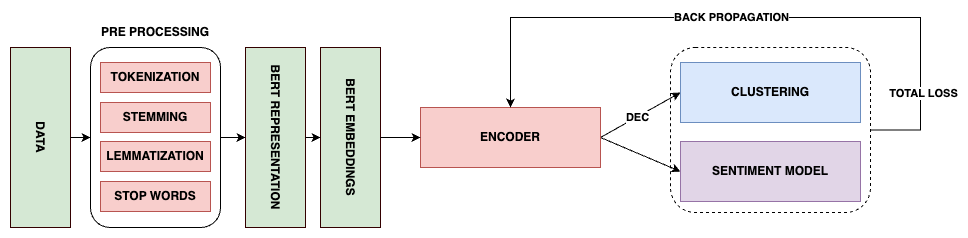
\includegraphics[width=0.85\textwidth]{assets/pics/MTL/FNN1.png}
    \caption{Diagram alur simulasi penelitian.}
    \label{fig:alur_simulasi}
\end{figure}

Proses dimulai dengan pengumpulan data ulasan yang kemudian melewati tahap
prapengolahan untuk menghasilkan data yang bersih. Data tersebut selanjutnya
diproses oleh BERT yang digunakan secara \textit{feature-based} dengan bobot
yang dibekukan, menghasilkan representasi vektor \texttt{[CLS]} berdimensi
768 untuk setiap dokumen. Representasi ini kemudian menjadi masukan bagi
\textit{autoencoder} untuk menghasilkan representasi laten berdimensi lebih
rendah.

Representasi laten yang dihasilkan digunakan secara bersamaan oleh dua jalur
tugas, yaitu analisis sentimen melalui \textit{sentiment head} dan
pendeteksian topik melalui \textit{Deep Embedded Clustering} (DEC). Setelah
pelatihan \textit{joint} selesai, kinerja dari kedua tugas dievaluasi dengan
metrik yang sesuai.

%-----------------------------------------------------------------------------%
\section{Data}
%-----------------------------------------------------------------------------%

Subbab ini menjelaskan data yang digunakan dalam penelitian, meliputi sumber
data, karakteristik dataset, serta tahapan persiapan data sebelum digunakan
dalam pelatihan model. Secara umum, proses pengolahan data dimulai dari
pengumpulan dataset ulasan, lalu dilanjutkan dengan prapengolahan teks,
pembentukan representasi menggunakan BERT, dan pembagian data.

%-----------------------------------------------------------------------------%
\subsection{Pengumpulan Data}
%-----------------------------------------------------------------------------%

Penelitian ini menggunakan dua dataset ulasan berbahasa Inggris, yaitu IMDB
Movie Reviews dan Yelp Review Dataset. Kedua dataset dipilih karena umum
digunakan sebagai \textit{benchmark} pada penelitian analisis sentimen dan
pendeteksian topik, serta keduanya memiliki label sentimen biner.

Dataset IMDB Movie Reviews terdiri dari 30.000 ulasan film yang diunggah oleh
\parencite{maas2011} dan tersedia secara publik melalui platform Hugging Face
dalam format Apache Arrow. Distribusi label sentimen pada dataset ini relatif
seimbang antara kelas positif dan negatif, sehingga cocok untuk tugas
klasifikasi biner.

Yelp Review Dataset memuat 50.000 ulasan pengguna terhadap berbagai jenis
layanan dan bisnis, termasuk restoran dan usaha ritel. Dataset ini tersedia
secara publik melalui platform Hugging Face yang diunggah oleh
\parencite{zhang2015} dalam format Apache Arrow dengan distribusi label
sentimen yang seimbang. Dalam penelitian ini, jumlah data Yelp dibatasi
hingga 30.000 sampel agar proporsional dengan jumlah data IMDB.

Kedua dataset memiliki label sentimen biner, dengan nilai 1 untuk sentimen
positif dan nilai 0 untuk sentimen negatif. Beberapa cuplikan ulasan dari
masing-masing dataset ditampilkan pada Tabel~\ref{tab:imdb_sample} dan
Tabel~\ref{tab:yelp_sample}.

\begin{table}[H]
    \centering
    \caption{Cuplikan data ulasan IMDB \parencite{maas2011}.}
    \label{tab:imdb_sample}
    \begin{tabular}{p{0.10\textwidth} p{0.73\textwidth} p{0.07\textwidth}}
        \hline
        \textbf{No} & \textbf{Text} & \textbf{Label} \\
        \hline
        1 &
        An absolute masterpiece. The storytelling is compelling from start
        to finish, and the performances are nothing short of extraordinary.
        Highly recommended to anyone who appreciates great cinema. & 1 \\
        \hline
        2 &
        A complete waste of time. The plot makes no sense, the acting is
        wooden, and the ending is thoroughly unsatisfying. Save yourself
        two hours and skip this one. & 0 \\
        \hline
        $\vdots$ & $\vdots$ & $\vdots$ \\
        \hline
        30.000 &
        The film captures a quiet kind of grief beautifully. Not much
        happens on the surface, but every scene carries emotional weight.
        A slow burn that rewards patient viewers. & 1 \\
        \hline
    \end{tabular}
\end{table}

\begin{table}[H]
    \centering
    \caption{Cuplikan data ulasan Yelp \parencite{zhang2015}.}
    \label{tab:yelp_sample}
    \begin{tabular}{p{0.10\textwidth} p{0.73\textwidth} p{0.07\textwidth}}
        \hline
        \textbf{No} & \textbf{Text} & \textbf{Label} \\
        \hline
        1 &
        Hands down the best ramen I have had outside of Japan. The broth
        is rich and complex, the noodles perfectly chewy. The staff were
        attentive without being intrusive. Will absolutely return. & 1 \\
        \hline
        2 &
        Ordered delivery and the food arrived nearly an hour late and
        completely cold. When I called to complain, the staff were
        dismissive. Would not order from here again. & 0 \\
        \hline
        $\vdots$ & $\vdots$ & $\vdots$ \\
        \hline
        30.000 &
        Decent enough for a quick lunch but nothing memorable. The portions
        are on the smaller side for the price, and the ambiance is a bit
        too noisy to hold a conversation comfortably. & 0 \\
        \hline
    \end{tabular}
\end{table}

%-----------------------------------------------------------------------------%
\subsection{Prapengolahan Data}
%-----------------------------------------------------------------------------%

Tahap prapengolahan bertujuan membersihkan teks dari elemen yang tidak
mengandung informasi bahasa sebelum diproses oleh BERT. Karena BERT
merupakan model berbasis \textit{transformer} yang menangkap hubungan
kontekstual antartoken, penelitian ini menerapkan prapengolahan yang
minimalis. Tahapan seperti \textit{stemming}, penghapusan \textit{stop words},
dan normalisasi tanda baca tidak diterapkan, karena kata-kata fungsional
seperti \textit{stop words} masih mengandung informasi kontekstual yang
relevan bagi model.

Selain itu, BERT menggunakan tokenisasi berbasis WordPiece yang mampu memecah
kata di luar kosakata menjadi unit \textit{subword}, sehingga normalisasi kata
secara manual tidak diperlukan. Prapengolahan pada penelitian ini difokuskan
pada pembersihan elemen non-linguistik tanpa menghilangkan kandungan informasi
dalam teks. Tahapan yang diterapkan adalah sebagai berikut.

\begin{enumerate}
    \item \textit{Casefolding}, yaitu mengubah seluruh teks menjadi
    huruf kecil untuk menghindari perbedaan representasi akibat variasi
    kapitalisasi.

    \item Penghapusan tag HTML, yaitu menghapus elemen HTML seperti
    \texttt{<br />} dan \texttt{<b>} yang tidak memiliki kandungan bahasa.

    \item Penghapusan URL, yaitu menghapus tautan dengan pola
    \texttt{http://...} atau \texttt{www....} karena tidak membawa informasi
    sentimen maupun topik.

    \item Penghapusan karakter non-ASCII, yaitu menghapus emoji,
    simbol unicode, dan karakter khusus yang dapat mengganggu proses
    tokenisasi.

    \item Normalisasi \textit{whitespace}, yaitu menyeragamkan
    spasi berlebih, karakter tab, dan baris baru menjadi satu spasi tunggal.
\end{enumerate}

Hasil dari tahap ini adalah teks yang bersih dari elemen non-linguistik
namun tetap mempertahankan struktur kalimat aslinya. Perbandingan teks
sebelum dan sesudah prapengolahan dapat dilihat pada
Tabel~\ref{tab:preprocessing}.

\begin{table}[H]
    \centering
    \caption{Contoh hasil prapengolahan pada dataset IMDB dan Yelp.}
    \label{tab:preprocessing}
    \begin{tabular}{p{0.47\textwidth} p{0.47\textwidth}}
        \hline
        \textbf{Sebelum Prapengolahan} & \textbf{Sesudah Prapengolahan} \\
        \hline
        \multicolumn{2}{l}{\textit{IMDB}} \\
        \hline
        An absolute MASTERPIECE. The storytelling is compelling.
        \texttt{<br />}Highly recommended to anyone who
        appreciates great cinema! &
        an absolute masterpiece. the storytelling is compelling.
        highly recommended to anyone who appreciates great cinema! \\
        \hline
        A complete waste of time. \texttt{<br />}Read the full
        review at http://www.filmcritic.org/reviews/2024 &
        a complete waste of time. read the full review at \\
        \hline
        \multicolumn{2}{l}{\textit{Yelp}} \\
        \hline
        Hands down the BEST ramen outside of Japan :) The broth
        is incredible! Check the menu at www.ramenhouse.com &
        hands down the best ramen outside of japan the broth
        is incredible! check the menu at \\
        \hline
        Ordered delivery \& the food arrived cold after 1hr.
        Staff were rude when I called :( Would NOT recommend. &
        ordered delivery the food arrived cold after 1hr.
        staff were rude when i called would not recommend. \\
        \hline
    \end{tabular}
\end{table}

Tabel~\ref{tab:preprocessing} menunjukkan bahwa perubahan yang dilakukan
terbatas pada penghapusan elemen non-linguistik dan penyeragaman format
teks, bukan penyederhanaan isi kalimat. Dengan demikian, kandungan
kontekstual dalam ulasan tetap terjaga untuk tahap ekstraksi fitur
menggunakan BERT.

%-----------------------------------------------------------------------------%
\subsection{Representasi Teks}
%-----------------------------------------------------------------------------%

Setelah prapengolahan, teks diubah menjadi representasi numerik melalui
dua tahap, yaitu tokenisasi dan ekstraksi fitur menggunakan BERT.
Representasi yang dihasilkan menjadi masukan bagi \textit{autoencoder}
pada tahap pelatihan berikutnya.

Tokenisasi dilakukan menggunakan tokenizer WordPiece dari model BERT
\textit{pre-trained}. Setiap teks dikonversi menjadi urutan \textit{token ID}
dengan panjang maksimum $t = 128$ token. Teks yang melebihi batas ini akan
dipotong (\textit{truncation}), sedangkan teks yang lebih pendek akan
ditambahkan token \texttt{[PAD]} bernilai 0 agar panjang urutan seragam.
Contoh hasil tokenisasi ditampilkan pada Tabel~\ref{tab:tokenisasi}.

\begin{table}[H]
    \centering
    \caption{Contoh proses tokenisasi menggunakan WordPiece BERT.}
    \label{tab:tokenisasi}
    \begin{tabular}{p{0.40\textwidth} p{0.52\textwidth}}
        \hline
        \textbf{Teks (hasil prapengolahan)} &
        \textbf{Hasil tokenisasi (\textit{token ID})} \\
        \hline
        an absolute masterpiece the storytelling is compelling &
        \texttt{[101, 2019, 7927, 4902, 1996, 4129, 2003, 17075,} \\
        & \texttt{102, 0, ..., 0]} \\
        \hline
    \end{tabular}
\end{table}

Urutan \textit{token ID} tersebut selanjutnya diproses oleh BERT untuk
menghasilkan representasi kontekstual. Model yang digunakan adalah BERT
\textit{pre-trained} dengan \textit{hidden size} 768 dan bobot yang
dibekukan sepenuhnya (\textit{frozen}). Dari keluaran BERT berupa matriks
berukuran $t \times 768$, diambil baris pertama yang bersesuaian dengan
token \texttt{[CLS]} sebagai representasi dokumen:

\begin{equation}
    \mathbf{f} = \mathbf{h}_1 \in \mathbb{R}^{768}
\end{equation}

\noindent dengan $\mathbf{h}_1$ adalah vektor keluaran BERT pada posisi
token \texttt{[CLS]}. Vektor $\mathbf{f}$ ini merepresentasikan konteks
global dokumen dan digunakan sebagai masukan bagi \textit{autoencoder}
pada tahap berikutnya. Contoh ilustrasi perubahan representasi dari
\textit{token ID} ke vektor BERT ditampilkan pada
Tabel~\ref{tab:bert_repr}.

\begin{table}[H]
    \centering
    \caption{Contoh representasi vektor \texttt{[CLS]} hasil ekstraksi BERT.}
    \label{tab:bert_repr}
    \begin{tabular}{p{0.40\textwidth} p{0.52\textwidth}}
        \hline
        \textbf{\textit{Token ID}} &
        \textbf{Representasi \texttt{[CLS]} $\mathbf{f} \in \mathbb{R}^{768}$} \\
        \hline
        \texttt{[101, 2019, 7927, 4902, ...]} &
        \texttt{[0.31, -0.17, 0.08, ..., -0.22]} \\
        \hline
    \end{tabular}
\end{table}

%-----------------------------------------------------------------------------%
\subsection{Pembagian Data}
%-----------------------------------------------------------------------------%

Setelah prapengolahan, data dari kedua dataset dibagi menjadi data latih
(\textit{training set}) dan data uji (\textit{test set}) dengan proporsi
80\% untuk data latih dan 20\% untuk data uji, mengacu pada skema yang
digunakan oleh \parencite{gowandi2021}. Pembagian ini dilakukan agar proses
pelatihan dan evaluasi model dapat dilakukan secara terpisah.

Data latih digunakan sebagai masukan dalam proses optimasi parameter model,
baik pada komponen analisis sentimen maupun pendeteksian topik. Data uji
digunakan untuk mengukur performa model pada data yang belum pernah dilihat
selama pelatihan.

%-----------------------------------------------------------------------------%
\section{Implementasi Model}
%-----------------------------------------------------------------------------%

Implementasi pada penelitian ini mencakup tiga model, yaitu JST-DEC sebagai
model yang diusulkan, NN-BERT sebagai model pembanding untuk analisis
sentimen, dan BERTopic sebagai model pembanding untuk pendeteksian topik.
JST-DEC dilatih melalui dua tahap, yaitu pra-pelatihan \textit{autoencoder}
dan \textit{joint training}. Seluruh model diimplementasikan menggunakan
Python dengan pustaka sebagaimana tercantum pada Tabel~\ref{tab:spesifikasi}.

%-----------------------------------------------------------------------------%
\subsection{Konfigurasi JST-DEC}
%-----------------------------------------------------------------------------%

JST-DEC terdiri dari \textit{autoencoder} dan komponen DEC. 
\textit{Autoencoder} digunakan untuk membentuk representasi laten dari vektor
\texttt{[CLS]} BERT, sedangkan DEC digunakan untuk membentuk klaster topik
pada ruang laten tersebut. Konfigurasi masing-masing komponen disajikan pada
Tabel~\ref{tab:config_ae} dan Tabel~\ref{tab:config_dec}.

\begin{table}[H]
    \centering
    \caption{Konfigurasi pra-pelatihan \textit{autoencoder}}
    \label{tab:config_ae}
    \renewcommand{\arraystretch}{1.15}
    \begin{tabular}{L{5.0cm} L{6.5cm}}
        \toprule
        \textbf{Parameter} & \textbf{Nilai} \\
        \midrule
        Arsitektur             & FC, simetris \\
        Dimensi lapisan        & $768{\to}2022{\to}2022{\to}256$ \\
        Dimensi laten          & 256 \\
        Fungsi aktivasi        & ReLU \\
        Fungsi \textit{loss}   & MSE \\
        \textit{Optimizer}     & Adam \\
        \textit{Learning rate} & $2 \times 10^{-3}$ \\
        \textit{Batch size}    & 128 \\
        Epoch                  & 30 \\
        \bottomrule
    \end{tabular}
\end{table}

\begin{table}[H]
    \centering
    \caption{Konfigurasi komponen DEC}
    \label{tab:config_dec}
    \renewcommand{\arraystretch}{1.15}
    \begin{tabular}{L{5.0cm} L{6.5cm}}
        \toprule
        \textbf{Parameter} & \textbf{Nilai} \\
        \midrule
        Lapisan klaster           & 1 \\
        Dimensi ruang klaster     & 256 \\
        Jumlah klaster ($K$)      & 30, 50, 80 \\
        \textit{Soft assignment}  & Student-$t$ \\
        Derajat kebebasan ($\nu$) & 1 \\
        \textit{Loss clustering}  & KL Divergence \\
        Inisialisasi centroid     & $k$-\textit{means} \\
        \bottomrule
    \end{tabular}
\end{table}

Dimensi masukan sebesar 768 mengikuti ukuran vektor \texttt{[CLS]} dari BERT.
Dimensi laten ditetapkan sebesar 256. Pada komponen DEC, jumlah klaster
yang diuji adalah 30, 50, dan 80 untuk melihat pengaruh variasi jumlah topik
terhadap hasil pendeteksian topik.

%-----------------------------------------------------------------------------%
\subsection{Konfigurasi \textit{Joint Training}}
%-----------------------------------------------------------------------------%

Setelah tahap pra-pelatihan, JST-DEC dilatih kembali melalui proses
\textit{joint training}. Pada tahap ini, model mengoptimasi dua tujuan secara
bersamaan, yaitu klasifikasi sentimen dan pembentukan klaster topik. Fungsi
\textit{loss} yang digunakan adalah

\[
\mathcal{L} = \eta\mathcal{L}_{\text{sent}} +
\gamma\mathcal{L}_{\text{clust}}.
\]

Konfigurasi \textit{joint training} JST-DEC disajikan pada
Tabel~\ref{tab:config_joint}.

\begin{table}[H]
    \centering
    \caption{Konfigurasi \textit{joint training} JST-DEC}
    \label{tab:config_joint}
    \renewcommand{\arraystretch}{1.15}
    \begin{tabular}{L{5.0cm} L{6.5cm}}
        \toprule
        \textbf{Parameter} & \textbf{Nilai} \\
        \midrule
        \textit{Learning rate}   & $5 \times 10^{-5}$ \\
        \textit{Batch size}      & 256 \\
        Iterasi maksimum         & 200 \\
        \textit{Update interval} & 20 \\
        Toleransi ($\tau$)       & $10^{-4}$ \\
        Bobot sentimen ($\eta$)  & 0{,}5 \\
        Bobot klaster ($\gamma$) & 0{,}5 \\
        \textit{Optimizer}       & SGD \\
        Jumlah topik ($K$)       & 30, 50, 80 \\
        \textit{Seed}            & 42 \\
        \bottomrule
    \end{tabular}
\end{table}

Nilai $\eta$ dan $\gamma$ ditetapkan sama besar, yaitu 0{,}5, sehingga tugas
analisis sentimen dan pendeteksian topik diberi bobot yang seimbang selama
pelatihan.

%-----------------------------------------------------------------------------%
\subsection{Konfigurasi Model Pembanding}
%-----------------------------------------------------------------------------%

Penelitian ini menggunakan dua model pembanding. NN-BERT digunakan sebagai
pembanding untuk tugas analisis sentimen, sedangkan BERTopic digunakan sebagai
pembanding untuk tugas pendeteksian topik.

%-----------------------------------------------------------------------------%
\subsubsection{NN-BERT}
%-----------------------------------------------------------------------------%

NN-BERT menggunakan representasi \texttt{[CLS]} dari BERT sebagai masukan
untuk lapisan klasifikasi. Konfigurasi model NN-BERT disajikan pada
Tabel~\ref{tab:config_nnbert}.

\begin{table}[H]
    \centering
    \caption{Konfigurasi model NN-BERT}
    \label{tab:config_nnbert}
    \renewcommand{\arraystretch}{1.15}
    \begin{tabular}{L{5.0cm} L{6.5cm}}
        \toprule
        \textbf{Parameter} & \textbf{Nilai} \\
        \midrule
        \textit{Encoder}        & BERT, \textit{frozen} \\
        Dimensi \textit{input}  & 768 (\texttt{[CLS]}) \\
        \textit{Classifier}     & FC, 1 lapisan \\
        Dimensi tersembunyi     & 256 \\
        Fungsi aktivasi         & ReLU \\
        Dimensi \textit{output} & 2 kelas \\
        Fungsi \textit{loss}    & \textit{Cross-Entropy} \\
        \textit{Optimizer}      & Adam \\
        \textit{Learning rate}  & $5 \times 10^{-5}$ \\
        \textit{Batch size}     & 256 \\
        Epoch                   & 10 \\
        \bottomrule
    \end{tabular}
\end{table}

%-----------------------------------------------------------------------------%
\subsubsection{BERTopic}
%-----------------------------------------------------------------------------%

BERTopic digunakan untuk membandingkan hasil pendeteksian topik. Model ini
menggunakan representasi berbasis BERT, reduksi dimensi dengan UMAP, dan
pengelompokan dengan HDBSCAN. Konfigurasinya disajikan pada
Tabel~\ref{tab:config_bertopic}.

\begin{table}[H]
    \centering
    \caption{Konfigurasi model BERTopic}
    \label{tab:config_bertopic}
    \renewcommand{\arraystretch}{1.15}
    \begin{tabular}{L{3.2cm} L{4.2cm} L{4.2cm}}
        \toprule
        \textbf{Komponen} & \textbf{Parameter} & \textbf{Nilai} \\
        \midrule
        \multirow{2}{*}{\textit{Embedding}}
            & Model     & {\small\texttt{bert-base-uncased}} \\
            & Dimensi   & 768 \\
        \midrule
        \multirow{4}{*}{UMAP}
            & \texttt{n\_neighbors}   & 15 \\
            & \texttt{n\_components}  & 5 \\
            & \texttt{min\_dist}      & 0{,}0 \\
            & Metrik                  & Kosinus \\
        \midrule
        \multirow{4}{*}{HDBSCAN}
            & \texttt{min\_cluster\_size}  & 10 \\
            & \texttt{min\_samples}        & 5 \\
            & Metrik                       & Euclidean \\
            & \texttt{prediction\_data}    & \texttt{True} \\
        \midrule
        \multirow{3}{*}{Topik}
            & Jumlah topik ($K$)   & 30, 50, 80 \\
            & Metode reduksi       & \texttt{nr\_topics} \\
            & Representasi topik   & c-TF-IDF \\
        \bottomrule
    \end{tabular}
\end{table}

%-----------------------------------------------------------------------------%
\section{Analisis Kinerja Model}
%-----------------------------------------------------------------------------%

Bagian ini menyajikan hasil evaluasi model pada dua tahap, yaitu
pra-pelatihan \textit{autoencoder} dan \textit{joint training}. Evaluasi
dilakukan pada dataset IMDB dan Yelp.

%-----------------------------------------------------------------------------%
\subsection{Analisis Kinerja Pra-pelatihan}
%-----------------------------------------------------------------------------%

Kinerja pra-pelatihan dievaluasi menggunakan nilai MSE pada data latih dan
data validasi. Hasil pra-pelatihan pada dataset IMDB dan Yelp disajikan pada
Tabel~\ref{tab:pretrain_loss_imdb} dan Tabel~\ref{tab:pretrain_loss_yelp}.

\begin{table}[H]
    \centering
    \caption{Perkembangan \textit{loss} pra-pelatihan pada dataset IMDB}
    \label{tab:pretrain_loss_imdb}
    \renewcommand{\arraystretch}{1.15}
    \begin{tabular}{C{2.0cm} C{3.5cm} C{3.5cm}}
        \toprule
        \textbf{Epoch}
        & \textbf{\textit{Train Loss}}
        & \textbf{\textit{Validation Loss}} \\
        \midrule
         1  & ... & ... \\
         5  & ... & ... \\
        10  & ... & ... \\
        15  & ... & ... \\
        20  & ... & ... \\
        25  & ... & ... \\
        30  & ... & ... \\
        \bottomrule
    \end{tabular}
\end{table}

\begin{table}[H]
    \centering
    \caption{Perkembangan \textit{loss} pra-pelatihan pada dataset Yelp}
    \label{tab:pretrain_loss_yelp}
    \renewcommand{\arraystretch}{1.15}
    \begin{tabular}{C{2.0cm} C{3.5cm} C{3.5cm}}
        \toprule
        \textbf{Epoch}
        & \textbf{\textit{Train Loss}}
        & \textbf{\textit{Validation Loss}} \\
        \midrule
         1  & ... & ... \\
         5  & ... & ... \\
        10  & ... & ... \\
        15  & ... & ... \\
        20  & ... & ... \\
        25  & ... & ... \\
        30  & ... & ... \\
        \bottomrule
    \end{tabular}
\end{table}

%-----------------------------------------------------------------------------%
\subsection{Analisis Kinerja \textit{Joint Training}}
%-----------------------------------------------------------------------------%

Kinerja \textit{joint training} dievaluasi berdasarkan dua kelompok metrik.
Tugas analisis sentimen dievaluasi menggunakan \textit{accuracy}, F1-score,
\textit{precision}, dan \textit{recall}. Tugas pendeteksian topik dievaluasi
menggunakan TC-NPMI dan TD.

%-----------------------------------------------------------------------------%
\subsubsection{Hasil Evaluasi pada Dataset IMDB}
%-----------------------------------------------------------------------------%

Hasil evaluasi pada dataset IMDB disajikan pada Tabel~\ref{tab:eval_imdb}.
Tanda ($-$) menunjukkan bahwa metrik tersebut tidak berlaku untuk model yang
bersangkutan.

\begin{table}[H]
    \centering
    \caption{Hasil evaluasi model pada dataset IMDB}
    \label{tab:eval_imdb}
    \renewcommand{\arraystretch}{1.15}
    \begin{tabular}{
        L{2.8cm}
        C{1.0cm}
        C{1.3cm}
        C{1.3cm}
        C{1.3cm}
        C{1.3cm}
        C{1.7cm}
        C{1.3cm}}
        \toprule
        \textbf{Model}
        & \textbf{\textit{K}}
        & \textbf{\textit{Accuracy}}
        & \textbf{\textit{F1}}
        & \textbf{\textit{Precision}}
        & \textbf{\textit{Recall}}
        & \textbf{TC-NPMI}
        & \textbf{TD} \\
        \midrule
        \multirow{3}{*}{JST-DEC}
          & 30 & ... & ... & ... & ... & ... & ... \\
          & 50 & ... & ... & ... & ... & ... & ... \\
          & 80 & ... & ... & ... & ... & ... & ... \\
        \midrule
        \multirow{3}{*}{BERTopic}
          & 30 & \multicolumn{4}{c}{$-$} & ... & ... \\
          & 50 & \multicolumn{4}{c}{$-$} & ... & ... \\
          & 80 & \multicolumn{4}{c}{$-$} & ... & ... \\
        \midrule
        NN-BERT
          & $-$ & ... & ... & ... & ... & \multicolumn{2}{c}{$-$} \\
        \bottomrule
    \end{tabular}
\end{table}

%-----------------------------------------------------------------------------%
\subsubsection{Hasil Evaluasi pada Dataset Yelp}
%-----------------------------------------------------------------------------%

Hasil evaluasi pada dataset Yelp disajikan pada Tabel~\ref{tab:eval_yelp}.
Format tabel dibuat sama dengan dataset IMDB agar hasil kedua dataset dapat
dibandingkan secara langsung.

\begin{table}[H]
    \centering
    \caption{Hasil evaluasi model pada dataset Yelp}
    \label{tab:eval_yelp}
    \renewcommand{\arraystretch}{1.15}
    \begin{tabular}{
        L{2.8cm}
        C{1.0cm}
        C{1.3cm}
        C{1.3cm}
        C{1.3cm}
        C{1.3cm}
        C{1.7cm}
        C{1.3cm}}
        \toprule
        \textbf{Model}
        & \textbf{\textit{K}}
        & \textbf{\textit{Accuracy}}
        & \textbf{\textit{F1}}
        & \textbf{\textit{Precision}}
        & \textbf{\textit{Recall}}
        & \textbf{TC-NPMI}
        & \textbf{TD} \\
        \midrule
        \multirow{3}{*}{JST-DEC}
          & 30 & ... & ... & ... & ... & ... & ... \\
          & 50 & ... & ... & ... & ... & ... & ... \\
          & 80 & ... & ... & ... & ... & ... & ... \\
        \midrule
        \multirow{3}{*}{BERTopic}
          & 30 & \multicolumn{4}{c}{$-$} & ... & ... \\
          & 50 & \multicolumn{4}{c}{$-$} & ... & ... \\
          & 80 & \multicolumn{4}{c}{$-$} & ... & ... \\
        \midrule
        NN-BERT
          & $-$ & ... & ... & ... & ... & \multicolumn{2}{c}{$-$} \\
        \bottomrule
    \end{tabular}
\end{table}
%---------------------------------------------------------------
\chapter{Penutup}
%---------------------------------------------------------------

%---------------------------------------------------------------
\section{Kesimpulan}
%---------------------------------------------------------------

Berdasarkan hasil penelitian yang telah dilakukan, dapat ditarik kesimpulan sebagai berikut.

\begin{enumerate}
    \item Model \textit{Joint Document-Level Sentiment-Topic Model} (JDST-DEC) berhasil dikembangkan dengan mengintegrasikan
     analisis sentimen dan pemodelan topik secara \textit{end-to-end} dalam satu kerangka \textit{multi-task learning}.
      Model memanfaatkan satu \textit{shared encoder} yang dipelajari secara bersama melalui 
      optimisasi \textit{sentiment loss} dan \textit{clustering loss}, sehingga mampu menghasilkan representasi 
      laten yang digunakan secara simultan oleh \textit{sentiment head} dan \textit{topic head} berbasis \textit{Deep Embedded Clustering} (DEC).

    \item Penerapan \textit{Deep Embedded Clustering} (DEC) pada \textit{topic head} berhasil membentuk representasi 
    topik dari representasi laten yang dihasilkan oleh \textit{shared encoder}. DEC mereduksi representasi BERT dari 
    768 dimensi menjadi 256 dimensi menggunakan \textit{autoencoder}, kemudian melakukan pembentukan klaster melalui 
    mekanisme \textit{soft assignment}. Pada evaluasi kualitas topik, JDST-DEC memperoleh nilai TC-NPMI tertinggi 
    sebesar 0{,}0803 pada dataset IMDB dan 0{,}0788 pada dataset Yelp. Hasil tersebut menunjukkan bahwa DEC mampu
     diintegrasikan dalam kerangka \textit{joint modelling}, meskipun kualitas topik yang dihasilkan masih dapat ditingkatkan.

    \item Pada tugas analisis sentimen, JDST-DEC memberikan performa yang lebih baik dibandingkan metode sebelumnya.
     Model secara konsisten memperoleh nilai \textit{accuracy} dan F1-score yang lebih tinggi dibandingkan NN-BERT 
     pada seluruh konfigurasi jumlah topik ($K=30$, $50$, dan $80$). Nilai F1-score terbaik yang diperoleh 
     mencapai 0{,}8986 pada dataset IMDB dan 0{,}9020 pada dataset Yelp, lebih tinggi dibandingkan NN-BERT yang 
     masing-masing memperoleh 0{,}8612 dan 0{,}8715. Hasil tersebut menunjukkan bahwa penerapan \textit{multi-task learning} 
     tidak menurunkan performa analisis sentimen, tetapi justru memberikan peningkatan dibandingkan model \textit{single-task}.

    \item Pada tugas pemodelan topik, JDST-DEC menunjukkan kualitas topik yang lebih baik dibandingkan MTL-GUI pada
     beberapa konfigurasi jumlah topik, namun masih berada di bawah BERTopic-KMeans berdasarkan metrik TC-NPMI maupun \textit{Topic Diversity}. 
     BERTopic-KMeans memperoleh TC-NPMI tertinggi sebesar 0{,}1874 pada IMDB dan 0{,}1465 pada Yelp, sedangkan nilai \textit{Topic Diversity} 
     tertinggi mencapai 0{,}9567 pada IMDB dan 0{,}7800 pada Yelp. Hasil tersebut menunjukkan bahwa meskipun DEC berhasil diintegrasikan 
     ke dalam model JDST, kualitas representasi topik yang dihasilkan masih belum mampu melampaui metode pemodelan topik khusus.
\end{enumerate}


%---------------------------------------------------------------
\section{Saran}
%---------------------------------------------------------------

Berdasarkan hasil dan keterbatasan pada penelitian ini, beberapa saran untuk
penelitian selanjutnya adalah sebagai berikut.

\begin{enumerate}
   \item Mengeksplorasi pengembangan arsitektur \textit{topic head} berbasis
    \textit{Deep Embedded Clustering} untuk meningkatkan kualitas representasi
    topik. Pengembangan dapat dilakukan melalui modifikasi struktur
    \textit{autoencoder}, mekanisme pembentukan distribusi target, maupun strategi
    optimisasi klaster.

    \item Mengeksplorasi pengembangan arsitektur \textit{sentiment head} untuk
    mendukung keseimbangan proses optimisasi antara tugas analisis sentimen
    dan klasterisasi. Berdasarkan hasil analisis \textit{multiloss}, perubahan
    pada komponen ini berpotensi membantu model mencapai keseimbangan yang
    lebih baik antara kualitas prediksi sentimen dan kualitas klaster.

    \item Mengeksplorasi strategi pembobotan \textit{loss} yang adaptif antara
    $\mathcal{L}_{\text{sent}}$ dan $\mathcal{L}_{\text{clust}}$ guna
    mengurangi \textit{trade-off} antara performa analisis sentimen dan
    kualitas klaster yang dihasilkan.
\end{enumerate}




%
% Daftar Pustaka
%\input{pustaka}

% Alternatif manajemen daftar pustaka dengan \bibliography
\renewbibmacro{in:}{}
\nocite{*}
\printbibliography[title={Daftar Pustaka}]

%
% Lampiran 
%
% \begin{appendix}
% 	\input{_internals/markLampiran}
% 	\setcounter{page}{2}
% 	%-----------------------------------------------------------------------------%
\chapter*{Lampiran 1 \\ Kode Program}
%-----------------------------------------------------------------------------%


\section*{Transformasi Data Text -> BERT Embeddings -> Cached Data [CDT]}
\lstinputlisting[language=Python, 
  caption={Full implementation of Cached Data Transformation (CDT).},
  label={lst:CDTBERT}]{src/code/data.py}


\section*{Arsitektur Model}
\lstinputlisting[language=Python, 
  caption={Full implementation of JDST-DEC (SEMTGPU).},
  label={lst:jdstdec}]{src/code/semtgpu.py}

\section*{JDST DEC Training Loop (IMDB and Yelp)}
\lstinputlisting[language=Python, 
  caption={Full implementation of JDST DEC training loop.},
  label={lst:jdstdec_train}]{src/code/jstdec.py}


\section*{BERT Topic Evaluation Loop (IMDB and Yelp)}
\lstinputlisting[language=Python, 
  caption={Full implementation of BERT Topic evaluation loop.},
  label={lst:bertopic_eval}]{src/code/bertopic.py}

\section*{MLTGUI Training Loop (IMDB and Yelp)}
\lstinputlisting[language=Python, 
  caption={Full implementation of MLTGUI training loop.},
  label={lst:mltgui_train}]{src/code/mltgui.py}
% \end{appendix}

\end{document}
